\documentclass{book}
\usepackage[a4paper,top=2.5cm,bottom=2.5cm,left=2.5cm,right=2.5cm]{geometry}
\usepackage{makeidx}
\usepackage{natbib}
\usepackage{graphicx}
\usepackage{multicol}
\usepackage{float}
\usepackage{listings}
\usepackage{color}
\usepackage{ifthen}
\usepackage[table]{xcolor}
\usepackage{textcomp}
\usepackage{alltt}
\usepackage{ifpdf}
\ifpdf
\usepackage[pdftex,
            pagebackref=true,
            colorlinks=true,
            linkcolor=blue,
            unicode
           ]{hyperref}
\else
\usepackage[ps2pdf,
            pagebackref=true,
            colorlinks=true,
            linkcolor=blue,
            unicode
           ]{hyperref}
\usepackage{pspicture}
\fi
\usepackage[utf8]{inputenc}
\usepackage{mathptmx}
\usepackage[scaled=.90]{helvet}
\usepackage{courier}
\usepackage{sectsty}
\usepackage{amssymb}
\usepackage[titles]{tocloft}
\usepackage{doxygen}
\lstset{language=C++,inputencoding=utf8,basicstyle=\footnotesize,breaklines=true,breakatwhitespace=true,tabsize=4,numbers=left }
\makeindex
\setcounter{tocdepth}{3}
\renewcommand{\footrulewidth}{0.4pt}
\renewcommand{\familydefault}{\sfdefault}
\hfuzz=15pt
\setlength{\emergencystretch}{15pt}
\hbadness=750
\tolerance=750
\begin{document}
\hypersetup{pageanchor=false,citecolor=blue}
\begin{titlepage}
\vspace*{7cm}
\begin{center}
{\Large Crumbler \\[1ex]\large v0.\-1 }\\
\vspace*{1cm}
{\large Generated by Doxygen 1.8.2}\\
\vspace*{0.5cm}
{\small Mon Dec 24 2012 18:01:45}\\
\end{center}
\end{titlepage}
\clearemptydoublepage
\pagenumbering{roman}
\tableofcontents
\clearemptydoublepage
\pagenumbering{arabic}
\hypersetup{pageanchor=true,citecolor=blue}
\chapter{Welcome to Crumbler}
\label{index}\hypertarget{index}{}\hypertarget{index_intro_sec}{}\section{Introduction}\label{index_intro_sec}
This is a project that will implement some of the famous and most widely used compression techniques. It will be delivered as a cross platform multi-\/functional library. we will also provide android, windows phone and i\-O\-S ports. The library is meant to be high performing, scalable, reliable.\par
 Contributors are welcome. Source is hosted at \href{https://github.com/sidharthamani/Android-Crumbler}{\tt https\-://github.\-com/sidharthamani/\-Android-\/\-Crumbler} \hypertarget{index_install_sec}{}\section{Installation}\label{index_install_sec}
Step 1\-: In order to install this library in your $\ast$unix/mac download zip package \par
 Step 2\-: type cd Crumbler \par
 Step 3\-: type make install \par
 Now it is installed. Follow instructions on \href{#}{\tt tutorials section} to completely tap into the power of Crumbler \hypertarget{index_xyz}{}\subsection{Getting Started}\label{index_xyz}
Go to \href{http://crumbler.sidharthamani.com/files.html}{\tt http\-://crumbler.\-sidharthamani.\-com/files.\-html} and check out the A\-P\-I documentation \par
 \hypertarget{index_ayz}{}\subsection{User Manual}\label{index_ayz}
Start using crumbler right away. See our User Manual \href{#}{\tt here. }
\chapter{Crumbler Project}
\label{proejct}
\hypertarget{proejct}{}
I will create a mailing list if there are actually some users and developers responding to this project 
\chapter{Coding Standards}
\label{coding_standards}
\hypertarget{coding_standards}{}
No single character names of functions or variables. Use full names, with multi word names seperated by underscore \par
 Variables -\/ struct structure\-\_\-type structure\-\_\-variable \par
 Functions -\/ Big\-\_\-\-Int$\ast$ init\-\_\-\-Big\-\_\-int(struct big\-\_\-integer value) \par
 
\chapter{Vacancies}
\label{vacancies}
\hypertarget{vacancies}{}
Need testers, developers, marketing guys \par
 contact -\/ \href{mailto:sidharthamn@gmail.com}{\tt sidharthamn@gmail.\-com} 
\chapter{License}
\label{license}
\hypertarget{license}{}
\href{http://creativecommons.org/licenses/by/3.0/deed.en_US}{\tt }\par
This work is licensed under a \href{http://creativecommons.org/licenses/by/3.0/deed.en_US}{\tt Creative Commons Attribution 3.\-0 Unported License}. 
\chapter{Developers}
\label{developers}
\hypertarget{developers}{}

\begin{DoxyEnumerate}
\item Sidhartha Mani, Carnegie Mellon grad student, contributor \par
 
\end{DoxyEnumerate}
\chapter{Module Index}
\section{Modules}
Here is a list of all modules\-:\begin{DoxyCompactList}
\item \contentsline{section}{Core}{\pageref{group__core}}{}
\item \contentsline{section}{Samples}{\pageref{group__samples}}{}
\end{DoxyCompactList}

\chapter{Namespace Index}
\section{Namespace List}
Here is a list of all namespaces with brief descriptions\-:\begin{DoxyCompactList}
\item\contentsline{section}{\hyperlink{namespacefrequency__sorter}{frequency\-\_\-sorter} }{\pageref{namespacefrequency__sorter}}{}
\item\contentsline{section}{\hyperlink{namespacefrequency__sorter__generator}{frequency\-\_\-sorter\-\_\-generator} }{\pageref{namespacefrequency__sorter__generator}}{}
\end{DoxyCompactList}

\chapter{Data Structure Index}
\section{Data Structures}
Here are the data structures with brief descriptions\-:\begin{DoxyCompactList}
\item\contentsline{section}{\hyperlink{struct_big___int}{Big\-\_\-\-Int} \\*A data structure that holds big integer values }{\pageref{struct_big___int}}{}
\item\contentsline{section}{\hyperlink{structdequeue}{dequeue} \\*Interface to the double ended queue }{\pageref{structdequeue}}{}
\item\contentsline{section}{\hyperlink{structsimple__prefix}{simple\-\_\-prefix} \\*Interface to the simple prefix functions }{\pageref{structsimple__prefix}}{}
\end{DoxyCompactList}

\chapter{File Index}
\section{File List}
Here is a list of all files with brief descriptions\-:\begin{DoxyCompactList}
\item\contentsline{section}{\hyperlink{doc_8c}{doc.\-c} \\*Contains documentation information. Contains no implementation }{\pageref{doc_8c}}{}
\item\contentsline{section}{/\-Users/sidharthamani/\-Crumbler/include/\hyperlink{big__integer_8h}{big\-\_\-integer.\-h} \\*Serves as the interface to Big Integer Implementation This file contains functions required to support big integer manipulation.\par
 Author \-: Sidhartha Mani\par
 Contact \-: \href{mailto:sidharthamn@gmail.com}{\tt sidharthamn@gmail.\-com} \par
 Last Updated \-: 23 Dec 2012 \par
 }{\pageref{big__integer_8h}}{}
\item\contentsline{section}{/\-Users/sidharthamani/\-Crumbler/include/\hyperlink{big__integer__impl_8h}{big\-\_\-integer\-\_\-impl.\-h} \\*The interface to the implementation of \hyperlink{big__integer__impl_8h_structbig__integer}{big\-\_\-integer} logic This file contains functions required to support the big integer manipulation functions.\par
 Author \-: Sidhartha Mani\par
 Contact \-: \href{mailto:sidharthamn@gmail.com}{\tt sidharthamn@gmail.\-com} \par
 Last Updated \-: 24 Dec 2012 \par
 }{\pageref{big__integer__impl_8h}}{}
\item\contentsline{section}{/\-Users/sidharthamani/\-Crumbler/include/\hyperlink{simple__prefix_8h}{simple\-\_\-prefix.\-h} \\*Serves as the interface to \hyperlink{structsimple__prefix}{simple\-\_\-prefix} This file contains functions required to support encoding and de-\/coding on files.\par
 Author \-: Sidhartha Mani\par
 Contact \-: \href{mailto:sidharthamn@gmail.com}{\tt sidharthamn@gmail.\-com} \par
 Last Updated \-: 23 Dec 2012 \par
 }{\pageref{simple__prefix_8h}}{}
\item\contentsline{section}{/\-Users/sidharthamani/\-Crumbler/include/\hyperlink{simple__prefix__impl_8h}{simple\-\_\-prefix\-\_\-impl.\-h} \\*Serves as the interface to the implementation of \hyperlink{structsimple__prefix}{simple\-\_\-prefix} tree This file contains functions required to support the encoding and de-\/coding functions.\par
 Author \-: Sidhartha Mani\par
 Contact \-: \href{mailto:sidharthamn@gmail.com}{\tt sidharthamn@gmail.\-com} \par
 Last Updated \-: 23 Dec 2012 \par
 }{\pageref{simple__prefix__impl_8h}}{}
\item\contentsline{section}{/\-Users/sidharthamani/\-Crumbler/include/collections/\hyperlink{binary__tree_8h}{binary\-\_\-tree.\-h} }{\pageref{binary__tree_8h}}{}
\item\contentsline{section}{/\-Users/sidharthamani/\-Crumbler/include/collections/\hyperlink{binary__tree__impl_8h}{binary\-\_\-tree\-\_\-impl.\-h} }{\pageref{binary__tree__impl_8h}}{}
\item\contentsline{section}{/\-Users/sidharthamani/\-Crumbler/include/collections/\hyperlink{dequeue_8h}{dequeue.\-h} \\*This file serves as the interface to dequeue functionality. \par
 It contains the interface to the various functions associated with the queue.\par
 Author \-: Sidhartha Mani\par
 Contact \-: \href{mailto:sidharthamn@gmail.com}{\tt sidharthamn@gmail.\-com} \par
 Last Updated \-: 2 Jan 2013\par
 }{\pageref{dequeue_8h}}{}
\item\contentsline{section}{/\-Users/sidharthamani/\-Crumbler/include/collections/\hyperlink{dequeue__impl_8h}{dequeue\-\_\-impl.\-h} \\*This file serves as the interface to the implementation of dequeue logic. \par
 It contains the implementation of various functions that the queue supports.\par
 Author \-: Sidhartha Mani\par
 Contact \-: \href{mailto:sidharthamn@gmail.com}{\tt sidharthamn@gmail.\-com} \par
 Last Updated \-: 28 Dec 2012\par
 }{\pageref{dequeue__impl_8h}}{}
\item\contentsline{section}{/\-Users/sidharthamani/\-Crumbler/include/collections/\hyperlink{double__edged__node_8h}{double\-\_\-edged\-\_\-node.\-h} \\*Serves as reusable code for dequeues and binary trees This file contains the definition of the double edged node, which will contain data, as well as links to a left and a right node.\par
 Author \-: Sidhartha Mani\par
 Contact \-: \href{mailto:sidharthamn@gmail.com}{\tt sidharthamn@gmail.\-com} \par
 Last Updated \-: 27 Dec 2012\par
 }{\pageref{double__edged__node_8h}}{}
\item\contentsline{section}{/\-Users/sidharthamani/\-Crumbler/include/huffman/\hyperlink{huffman_8h}{huffman.\-h} }{\pageref{huffman_8h}}{}
\item\contentsline{section}{/\-Users/sidharthamani/\-Crumbler/include/huffman/\hyperlink{huffman__impl_8h}{huffman\-\_\-impl.\-h} }{\pageref{huffman__impl_8h}}{}
\item\contentsline{section}{/\-Users/sidharthamani/\-Crumbler/res/scripts/\hyperlink{frequency__sorter_8py}{frequency\-\_\-sorter.\-py} }{\pageref{frequency__sorter_8py}}{}
\item\contentsline{section}{/\-Users/sidharthamani/\-Crumbler/res/scripts/\hyperlink{frequency__sorter__generator_8py}{frequency\-\_\-sorter\-\_\-generator.\-py} }{\pageref{frequency__sorter__generator_8py}}{}
\item\contentsline{section}{/\-Users/sidharthamani/\-Crumbler/samples/\hyperlink{big__integer__comparator_8c}{big\-\_\-integer\-\_\-comparator.\-c} \\*A sample implementation of \hyperlink{big__integer__impl_8h_structbig__integer}{big\-\_\-integer} comparison using crumbler library \par
 Author \-: Sidhartha Mani \par
 Contact \-: \href{mailto:sidharthamn@gmail.com}{\tt sidharthamn@gmail.\-com} \par
 Last updated on \-: 24 Dec 2012 }{\pageref{big__integer__comparator_8c}}{}
\item\contentsline{section}{/\-Users/sidharthamani/\-Crumbler/samples/\hyperlink{dequeue__impl__sample_8c}{dequeue\-\_\-impl\-\_\-sample.\-c} \\*A sample implementation of enqueing and dequing using crumbler library \par
 Author \-: Sidhartha Mani \par
 Contact \-: \href{mailto:sidharthamn@gmail.com}{\tt sidharthamn@gmail.\-com} \par
 Last updated on \-: 29 Dec 2012 }{\pageref{dequeue__impl__sample_8c}}{}
\item\contentsline{section}{/\-Users/sidharthamani/\-Crumbler/samples/\hyperlink{simple__prefix__decoder_8c}{simple\-\_\-prefix\-\_\-decoder.\-c} \\*A sample implementation of simple prefix decoding using crumbler library \par
 Author \-: Sidhartha Mani \par
 Contact \-: \href{mailto:sidharthamn@gmail.com}{\tt sidharthamn@gmail.\-com} \par
 Last updated on \-: 24 Dec 2012 }{\pageref{simple__prefix__decoder_8c}}{}
\item\contentsline{section}{/\-Users/sidharthamani/\-Crumbler/samples/\hyperlink{simple__prefix__encoder_8c}{simple\-\_\-prefix\-\_\-encoder.\-c} \\*A sample implementation of simple prefix encoding using crumbler library \par
 Author \-: Sidhartha Mani \par
 Contact \-: \href{mailto:sidharthamn@gmail.com}{\tt sidharthamn@gmail.\-com} \par
 Last updated on \-: 24 Dec 2012 }{\pageref{simple__prefix__encoder_8c}}{}
\item\contentsline{section}{/\-Users/sidharthamani/\-Crumbler/src/\hyperlink{big__integer_8c}{big\-\_\-integer.\-c} \\*The interface to the implementation of big integer logic This file contains functions required to interface with the big integer manipulation functions.\par
 Author \-: Sidhartha Mani\par
 Contact \-: \href{mailto:sidharthamn@gmail.com}{\tt sidharthamn@gmail.\-com} \par
 Last Updated \-: 24 Dec 2012 \par
 }{\pageref{big__integer_8c}}{}
\item\contentsline{section}{/\-Users/sidharthamani/\-Crumbler/src/\hyperlink{big__integer__impl_8c}{big\-\_\-integer\-\_\-impl.\-c} \\*The implementation of \hyperlink{big__integer__impl_8h_structbig__integer}{big\-\_\-integer} logic This file contains functions required to support the big integer manipulation functions.\par
 Author \-: Sidhartha Mani\par
 Contact \-: \href{mailto:sidharthamn@gmail.com}{\tt sidharthamn@gmail.\-com} \par
 Last Updated \-: 24 Dec 2012 \par
 }{\pageref{big__integer__impl_8c}}{}
\item\contentsline{section}{/\-Users/sidharthamani/\-Crumbler/src/\hyperlink{simple__prefix_8c}{simple\-\_\-prefix.\-c} \\*The interface to \hyperlink{structsimple__prefix}{simple\-\_\-prefix} implementation This file contains functions required to interface with other functions for encoding and decoding files\par
 Author \-: Sidhartha Mani\par
 Contact \-: \href{mailto:sidharthamn@gmail.com}{\tt sidharthamn@gmail.\-com} \par
 Last Updated \-: 24 Dec 2012 \par
 }{\pageref{simple__prefix_8c}}{}
\item\contentsline{section}{/\-Users/sidharthamani/\-Crumbler/src/\hyperlink{simple__prefix__impl_8c}{simple\-\_\-prefix\-\_\-impl.\-c} \\*The implementation of \hyperlink{structsimple__prefix}{simple\-\_\-prefix} tree This file contains functions required to support the encoding and de-\/coding functions.\par
 Author \-: Sidhartha Mani\par
 Contact \-: \href{mailto:sidharthamn@gmail.com}{\tt sidharthamn@gmail.\-com} \par
 Last Updated \-: 23 Dec 2012 \par
 }{\pageref{simple__prefix__impl_8c}}{}
\item\contentsline{section}{/\-Users/sidharthamani/\-Crumbler/src/collections/\hyperlink{binary__tree_8c}{binary\-\_\-tree.\-c} }{\pageref{binary__tree_8c}}{}
\item\contentsline{section}{/\-Users/sidharthamani/\-Crumbler/src/collections/\hyperlink{binary__tree__impl_8c}{binary\-\_\-tree\-\_\-impl.\-c} }{\pageref{binary__tree__impl_8c}}{}
\item\contentsline{section}{/\-Users/sidharthamani/\-Crumbler/src/collections/\hyperlink{dequeue_8c}{dequeue.\-c} \\*This file serves as the interface to dequeue functionality. \par
 It contains the interface to the various functions associated with the queue.\par
 Author \-: Sidhartha Mani\par
 Contact \-: \href{mailto:sidharthamn@gmail.com}{\tt sidharthamn@gmail.\-com} \par
 Last Updated \-: 2 Jan 2013\par
 }{\pageref{dequeue_8c}}{}
\item\contentsline{section}{/\-Users/sidharthamani/\-Crumbler/src/collections/\hyperlink{dequeue__impl_8c}{dequeue\-\_\-impl.\-c} \\*This file contains the implementation of dequeue logic \par
 It serves as the implementation of various functions that the queue supports.\par
 Author \-: Sidhartha Mani\par
 Contact \-: \href{mailto:sidharthamn@gmail.com}{\tt sidharthamn@gmail.\-com} \par
 Last Updated \-: 28 Dec 2012\par
 }{\pageref{dequeue__impl_8c}}{}
\item\contentsline{section}{/\-Users/sidharthamani/\-Crumbler/src/huffman/\hyperlink{huffman_8c}{huffman.\-c} }{\pageref{huffman_8c}}{}
\item\contentsline{section}{/\-Users/sidharthamani/\-Crumbler/src/huffman/\hyperlink{huffman__impl_8c}{huffman\-\_\-impl.\-c} }{\pageref{huffman__impl_8c}}{}
\end{DoxyCompactList}

\chapter{Module Documentation}
\hypertarget{group__core}{\section{Core}
\label{group__core}\index{Core@{Core}}
}


Contains all the core methods and structures for use in different parts of the Crumbler Platform.  


\subsection*{Files}
\begin{DoxyCompactItemize}
\item 
file \hyperlink{big__integer_8h}{big\-\_\-integer.\-h}
\begin{DoxyCompactList}\small\item\em serves as the interface to Big Integer Implementation This file contains functions required to support big integer manipulation.\par
 Author \-: Sidhartha Mani\par
 Contact \-: \href{mailto:sidharthamn@gmail.com}{\tt sidharthamn@gmail.\-com} \par
 Last Updated \-: 23 Dec 2012 \par
 \end{DoxyCompactList}\item 
file \hyperlink{big__integer__impl_8h}{big\-\_\-integer\-\_\-impl.\-h}
\begin{DoxyCompactList}\small\item\em The interface to the implementation of \hyperlink{big__integer__impl_8h_structbig__integer}{big\-\_\-integer} logic This file contains functions required to support the big integer manipulation functions.\par
 Author \-: Sidhartha Mani\par
 Contact \-: \href{mailto:sidharthamn@gmail.com}{\tt sidharthamn@gmail.\-com} \par
 Last Updated \-: 24 Dec 2012 \par
 \end{DoxyCompactList}\item 
file \hyperlink{simple__prefix_8h}{simple\-\_\-prefix.\-h}
\begin{DoxyCompactList}\small\item\em serves as the interface to \hyperlink{structsimple__prefix}{simple\-\_\-prefix} This file contains functions required to support encoding and de-\/coding on files.\par
 Author \-: Sidhartha Mani\par
 Contact \-: \href{mailto:sidharthamn@gmail.com}{\tt sidharthamn@gmail.\-com} \par
 Last Updated \-: 23 Dec 2012 \par
 \end{DoxyCompactList}\item 
file \hyperlink{simple__prefix__impl_8h}{simple\-\_\-prefix\-\_\-impl.\-h}
\begin{DoxyCompactList}\small\item\em serves as the interface to the implementation of \hyperlink{structsimple__prefix}{simple\-\_\-prefix} tree This file contains functions required to support the encoding and de-\/coding functions.\par
 Author \-: Sidhartha Mani\par
 Contact \-: \href{mailto:sidharthamn@gmail.com}{\tt sidharthamn@gmail.\-com} \par
 Last Updated \-: 23 Dec 2012 \par
 \end{DoxyCompactList}\item 
file \hyperlink{big__integer_8c}{big\-\_\-integer.\-c}
\begin{DoxyCompactList}\small\item\em The interface to the implementation of big integer logic This file contains functions required to interface with the big integer manipulation functions.\par
 Author \-: Sidhartha Mani\par
 Contact \-: \href{mailto:sidharthamn@gmail.com}{\tt sidharthamn@gmail.\-com} \par
 Last Updated \-: 24 Dec 2012 \par
 \end{DoxyCompactList}\item 
file \hyperlink{big__integer__impl_8c}{big\-\_\-integer\-\_\-impl.\-c}
\begin{DoxyCompactList}\small\item\em The implementation of \hyperlink{big__integer__impl_8h_structbig__integer}{big\-\_\-integer} logic This file contains functions required to support the big integer manipulation functions.\par
 Author \-: Sidhartha Mani\par
 Contact \-: \href{mailto:sidharthamn@gmail.com}{\tt sidharthamn@gmail.\-com} \par
 Last Updated \-: 24 Dec 2012 \par
 \end{DoxyCompactList}\item 
file \hyperlink{simple__prefix_8c}{simple\-\_\-prefix.\-c}
\begin{DoxyCompactList}\small\item\em The interface to \hyperlink{structsimple__prefix}{simple\-\_\-prefix} implementation This file contains functions required to interface with other functions for encoding and decoding files\par
 Author \-: Sidhartha Mani\par
 Contact \-: \href{mailto:sidharthamn@gmail.com}{\tt sidharthamn@gmail.\-com} \par
 Last Updated \-: 24 Dec 2012 \par
 \end{DoxyCompactList}\item 
file \hyperlink{simple__prefix__impl_8c}{simple\-\_\-prefix\-\_\-impl.\-c}
\begin{DoxyCompactList}\small\item\em The implementation of \hyperlink{structsimple__prefix}{simple\-\_\-prefix} tree This file contains functions required to support the encoding and de-\/coding functions.\par
 Author \-: Sidhartha Mani\par
 Contact \-: \href{mailto:sidharthamn@gmail.com}{\tt sidharthamn@gmail.\-com} \par
 Last Updated \-: 23 Dec 2012 \par
 \end{DoxyCompactList}\end{DoxyCompactItemize}


\subsection{Detailed Description}
Contains all the core methods and structures for use in different parts of the Crumbler Platform. 
\hypertarget{group__samples}{\section{Samples}
\label{group__samples}\index{Samples@{Samples}}
}


Contains all the sample implementation of the functions provided in the Crumbler Platform.  


\subsection*{Files}
\begin{DoxyCompactItemize}
\item 
file \hyperlink{big__integer__comparator_8c}{big\-\_\-integer\-\_\-comparator.\-c}
\begin{DoxyCompactList}\small\item\em A sample implementation of \hyperlink{big__integer__impl_8h_structbig__integer}{big\-\_\-integer} comparison using crumbler library \par
 Author \-: Sidhartha Mani \par
 Contact \-: \href{mailto:sidharthamn@gmail.com}{\tt sidharthamn@gmail.\-com} \par
 Last updated on \-: 24 Dec 2012. \end{DoxyCompactList}\item 
file \hyperlink{simple__prefix__encoder_8c}{simple\-\_\-prefix\-\_\-encoder.\-c}
\begin{DoxyCompactList}\small\item\em A sample implementation of simple prefix decoding using crumbler library \par
 Author \-: Sidhartha Mani \par
 Contact \-: \href{mailto:sidharthamn@gmail.com}{\tt sidharthamn@gmail.\-com} \par
 Last updated on \-: 24 Dec 2012. \end{DoxyCompactList}\item 
file \hyperlink{simple__prefix__encoder_8c}{simple\-\_\-prefix\-\_\-encoder.\-c}
\begin{DoxyCompactList}\small\item\em A sample implementation of simple prefix decoding using crumbler library \par
 Author \-: Sidhartha Mani \par
 Contact \-: \href{mailto:sidharthamn@gmail.com}{\tt sidharthamn@gmail.\-com} \par
 Last updated on \-: 24 Dec 2012. \end{DoxyCompactList}\end{DoxyCompactItemize}


\subsection{Detailed Description}
Contains all the sample implementation of the functions provided in the Crumbler Platform. 
\chapter{Namespace Documentation}
\hypertarget{namespacefrequency__sorter}{\section{frequency\-\_\-sorter Namespace Reference}
\label{namespacefrequency__sorter}\index{frequency\-\_\-sorter@{frequency\-\_\-sorter}}
}

\hypertarget{namespacefrequency__sorter__generator}{\section{frequency\-\_\-sorter\-\_\-generator Namespace Reference}
\label{namespacefrequency__sorter__generator}\index{frequency\-\_\-sorter\-\_\-generator@{frequency\-\_\-sorter\-\_\-generator}}
}
\subsection*{Functions}
\begin{DoxyCompactItemize}
\item 
def \hyperlink{namespacefrequency__sorter__generator_a4e5d2ba44e86d8d0b09d71d55d8caecb}{construct\-\_\-sorted\-\_\-frequencies\-\_\-hash\-\_\-map}
\end{DoxyCompactItemize}
\subsection*{Variables}
\begin{DoxyCompactItemize}
\item 
tuple \hyperlink{namespacefrequency__sorter__generator_af10bac427cf4eda50c22bfc352141c53}{file\-\_\-input} open('''frequencies''','''r''')
\item 
tuple \hyperlink{namespacefrequency__sorter__generator_a46abc2f5c61db548b0851ad685b29a49}{sorted\-\_\-frequencies\-\_\-tree} \hyperlink{namespacefrequency__sorter__generator_a4e5d2ba44e86d8d0b09d71d55d8caecb}{construct\-\_\-sorted\-\_\-frequencies\-\_\-hash\-\_\-map}(file\-\_\-input.\-read())
\item 
tuple \hyperlink{namespacefrequency__sorter__generator_a25e9eabadb6d4f7c84eca83f978cfd4f}{file\-\_\-output} open('''frequency\-\_\-sorter.\-py''','''w''')
\end{DoxyCompactItemize}


\subsection{Function Documentation}
\hypertarget{namespacefrequency__sorter__generator_a4e5d2ba44e86d8d0b09d71d55d8caecb}{\index{frequency\-\_\-sorter\-\_\-generator@{frequency\-\_\-sorter\-\_\-generator}!construct\-\_\-sorted\-\_\-frequencies\-\_\-hash\-\_\-map@{construct\-\_\-sorted\-\_\-frequencies\-\_\-hash\-\_\-map}}
\index{construct\-\_\-sorted\-\_\-frequencies\-\_\-hash\-\_\-map@{construct\-\_\-sorted\-\_\-frequencies\-\_\-hash\-\_\-map}!frequency_sorter_generator@{frequency\-\_\-sorter\-\_\-generator}}
\subsubsection[{construct\-\_\-sorted\-\_\-frequencies\-\_\-hash\-\_\-map}]{\setlength{\rightskip}{0pt plus 5cm}def frequency\-\_\-sorter\-\_\-generator.\-construct\-\_\-sorted\-\_\-frequencies\-\_\-hash\-\_\-map (
\begin{DoxyParamCaption}
\item[{}]{file\-\_\-input}
\end{DoxyParamCaption}
)}}\label{namespacefrequency__sorter__generator_a4e5d2ba44e86d8d0b09d71d55d8caecb}


Definition at line 3 of file frequency\-\_\-sorter\-\_\-generator.\-py.


\begin{DoxyCode}
3 
4 \textcolor{keyword}{def }\hyperlink{namespacefrequency__sorter__generator_a4e5d2ba44e86d8d0b09d71d55d8caecb}{construct\_sorted\_frequencies\_hash\_map}(
      file\_input):
5     file\_input = file\_input.split(\textcolor{stringliteral}{''','''})
6     return\_value = \textcolor{stringliteral}{'''\{'''}
7     \textcolor{keywordflow}{for} values \textcolor{keywordflow}{in} file\_input:
8         return\_value += (\textcolor{stringliteral}{"""'"""} + values.split(\textcolor{stringliteral}{''':'''})[0] + \textcolor{stringliteral}{"""'"""} + \textcolor{stringliteral}{''' : 
      '''} + values.split(\textcolor{stringliteral}{''':'''})[1])
9         return\_value += (\textcolor{stringliteral}{''', '''})
10     return\_value = return\_value[:-2]
11     return\_value += (\textcolor{stringliteral}{'''\}'''})
12     \textcolor{keywordflow}{return} return\_value

\end{DoxyCode}


\subsection{Variable Documentation}
\hypertarget{namespacefrequency__sorter__generator_af10bac427cf4eda50c22bfc352141c53}{\index{frequency\-\_\-sorter\-\_\-generator@{frequency\-\_\-sorter\-\_\-generator}!file\-\_\-input@{file\-\_\-input}}
\index{file\-\_\-input@{file\-\_\-input}!frequency_sorter_generator@{frequency\-\_\-sorter\-\_\-generator}}
\subsubsection[{file\-\_\-input}]{\setlength{\rightskip}{0pt plus 5cm}tuple file\-\_\-input open('''frequencies''','''r''')}}\label{namespacefrequency__sorter__generator_af10bac427cf4eda50c22bfc352141c53}


Definition at line 13 of file frequency\-\_\-sorter\-\_\-generator.\-py.

\hypertarget{namespacefrequency__sorter__generator_a25e9eabadb6d4f7c84eca83f978cfd4f}{\index{frequency\-\_\-sorter\-\_\-generator@{frequency\-\_\-sorter\-\_\-generator}!file\-\_\-output@{file\-\_\-output}}
\index{file\-\_\-output@{file\-\_\-output}!frequency_sorter_generator@{frequency\-\_\-sorter\-\_\-generator}}
\subsubsection[{file\-\_\-output}]{\setlength{\rightskip}{0pt plus 5cm}tuple file\-\_\-output open('''frequency\-\_\-sorter.\-py''','''w''')}}\label{namespacefrequency__sorter__generator_a25e9eabadb6d4f7c84eca83f978cfd4f}


Definition at line 15 of file frequency\-\_\-sorter\-\_\-generator.\-py.

\hypertarget{namespacefrequency__sorter__generator_a46abc2f5c61db548b0851ad685b29a49}{\index{frequency\-\_\-sorter\-\_\-generator@{frequency\-\_\-sorter\-\_\-generator}!sorted\-\_\-frequencies\-\_\-tree@{sorted\-\_\-frequencies\-\_\-tree}}
\index{sorted\-\_\-frequencies\-\_\-tree@{sorted\-\_\-frequencies\-\_\-tree}!frequency_sorter_generator@{frequency\-\_\-sorter\-\_\-generator}}
\subsubsection[{sorted\-\_\-frequencies\-\_\-tree}]{\setlength{\rightskip}{0pt plus 5cm}tuple sorted\-\_\-frequencies\-\_\-tree {\bf construct\-\_\-sorted\-\_\-frequencies\-\_\-hash\-\_\-map}(file\-\_\-input.\-read())}}\label{namespacefrequency__sorter__generator_a46abc2f5c61db548b0851ad685b29a49}


Definition at line 14 of file frequency\-\_\-sorter\-\_\-generator.\-py.


\chapter{Data Structure Documentation}
\hypertarget{struct_big___int}{\section{Big\-\_\-\-Int Struct Reference}
\label{struct_big___int}\index{Big\-\_\-\-Int@{Big\-\_\-\-Int}}
}


A data structure that holds big integer values.  




{\ttfamily \#include $<$big\-\_\-integer.\-h$>$}



Collaboration diagram for Big\-\_\-\-Int\-:\nopagebreak
\begin{figure}[H]
\begin{center}
\leavevmode
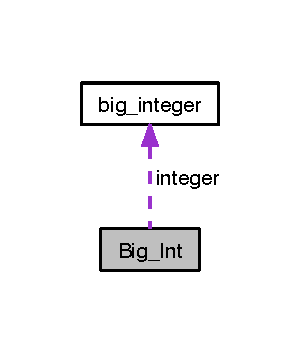
\includegraphics[width=145pt]{struct_big___int__coll__graph}
\end{center}
\end{figure}
\subsection*{Data Fields}
\begin{DoxyCompactItemize}
\item 
struct \hyperlink{big__integer__impl_8h_structbig__integer}{big\-\_\-integer} $\ast$ \hyperlink{struct_big___int_af78495b20eeda6242727ea99032693c2}{integer}
\item 
char $\ast$($\ast$ \hyperlink{struct_big___int_ac8d650b12656faee53d9ebd863e9fe8f}{get\-\_\-integer} )(struct \hyperlink{struct_big___int}{Big\-\_\-\-Int} $\ast$x)
\item 
int($\ast$ \hyperlink{struct_big___int_ae06ba678ba07ecdac264605bc8576da2}{get\-\_\-sign} )(struct \hyperlink{struct_big___int}{Big\-\_\-\-Int} $\ast$x)
\item 
void($\ast$ \hyperlink{struct_big___int_a34a65fb8d8cc2acf5a14a18c420ee774}{set\-\_\-integer} )(struct \hyperlink{struct_big___int}{Big\-\_\-\-Int} $\ast$this, char $\ast$\hyperlink{struct_big___int_af78495b20eeda6242727ea99032693c2}{integer})
\item 
void($\ast$ \hyperlink{struct_big___int_a70cf790b3af136aad25fa028cde3e801}{set\-\_\-sign} )(struct \hyperlink{struct_big___int}{Big\-\_\-\-Int} $\ast$this, int sign)
\end{DoxyCompactItemize}


\subsection{Detailed Description}
A data structure that holds big integer values. 

Definition at line 18 of file big\-\_\-integer.\-h.



\subsection{Field Documentation}
\hypertarget{struct_big___int_ac8d650b12656faee53d9ebd863e9fe8f}{\index{Big\-\_\-\-Int@{Big\-\_\-\-Int}!get\-\_\-integer@{get\-\_\-integer}}
\index{get\-\_\-integer@{get\-\_\-integer}!Big_Int@{Big\-\_\-\-Int}}
\subsubsection[{get\-\_\-integer}]{\setlength{\rightskip}{0pt plus 5cm}char$\ast$($\ast$ get\-\_\-integer)(struct {\bf Big\-\_\-\-Int} $\ast$x)}}\label{struct_big___int_ac8d650b12656faee53d9ebd863e9fe8f}
an accesor function which returns the integer as a character array 

Definition at line 23 of file big\-\_\-integer.\-h.

\hypertarget{struct_big___int_ae06ba678ba07ecdac264605bc8576da2}{\index{Big\-\_\-\-Int@{Big\-\_\-\-Int}!get\-\_\-sign@{get\-\_\-sign}}
\index{get\-\_\-sign@{get\-\_\-sign}!Big_Int@{Big\-\_\-\-Int}}
\subsubsection[{get\-\_\-sign}]{\setlength{\rightskip}{0pt plus 5cm}int($\ast$ get\-\_\-sign)(struct {\bf Big\-\_\-\-Int} $\ast$x)}}\label{struct_big___int_ae06ba678ba07ecdac264605bc8576da2}
an accesor function which returns the sign as an integer value. 1 \-: positive and '0', 2\-: negative, 

Definition at line 25 of file big\-\_\-integer.\-h.

\hypertarget{struct_big___int_af78495b20eeda6242727ea99032693c2}{\index{Big\-\_\-\-Int@{Big\-\_\-\-Int}!integer@{integer}}
\index{integer@{integer}!Big_Int@{Big\-\_\-\-Int}}
\subsubsection[{integer}]{\setlength{\rightskip}{0pt plus 5cm}struct {\bf big\-\_\-integer}$\ast$ integer}}\label{struct_big___int_af78495b20eeda6242727ea99032693c2}
an instances of the internal \hyperlink{big__integer__impl_8h_structbig__integer}{big\-\_\-integer} type 

Definition at line 21 of file big\-\_\-integer.\-h.

\hypertarget{struct_big___int_a34a65fb8d8cc2acf5a14a18c420ee774}{\index{Big\-\_\-\-Int@{Big\-\_\-\-Int}!set\-\_\-integer@{set\-\_\-integer}}
\index{set\-\_\-integer@{set\-\_\-integer}!Big_Int@{Big\-\_\-\-Int}}
\subsubsection[{set\-\_\-integer}]{\setlength{\rightskip}{0pt plus 5cm}void($\ast$ set\-\_\-integer)(struct {\bf Big\-\_\-\-Int} $\ast$this, char $\ast${\bf integer})}}\label{struct_big___int_a34a65fb8d8cc2acf5a14a18c420ee774}
a function to set the integer value to the value in param 2 

Definition at line 27 of file big\-\_\-integer.\-h.

\hypertarget{struct_big___int_a70cf790b3af136aad25fa028cde3e801}{\index{Big\-\_\-\-Int@{Big\-\_\-\-Int}!set\-\_\-sign@{set\-\_\-sign}}
\index{set\-\_\-sign@{set\-\_\-sign}!Big_Int@{Big\-\_\-\-Int}}
\subsubsection[{set\-\_\-sign}]{\setlength{\rightskip}{0pt plus 5cm}void($\ast$ set\-\_\-sign)(struct {\bf Big\-\_\-\-Int} $\ast$this, int sign)}}\label{struct_big___int_a70cf790b3af136aad25fa028cde3e801}
a function to set sign to the value in param 2 

Definition at line 29 of file big\-\_\-integer.\-h.



The documentation for this struct was generated from the following file\-:\begin{DoxyCompactItemize}
\item 
/\-Users/sidharthamani/\-Crumbler/include/\hyperlink{big__integer_8h}{big\-\_\-integer.\-h}\end{DoxyCompactItemize}

\hypertarget{structsimple__prefix}{\section{simple\-\_\-prefix Struct Reference}
\label{structsimple__prefix}\index{simple\-\_\-prefix@{simple\-\_\-prefix}}
}


the interface to the simple prefix functions  




{\ttfamily \#include $<$simple\-\_\-prefix.\-h$>$}

\subsection*{Data Fields}
\begin{DoxyCompactItemize}
\item 
F\-I\-L\-E $\ast$($\ast$ \hyperlink{structsimple__prefix_a73d0a239981b130553964b3839c20bdf}{encode\-\_\-file} )(char $\ast$, char $\ast$)
\item 
F\-I\-L\-E $\ast$($\ast$ \hyperlink{structsimple__prefix_a58708e15f01f3be37e12d3194e953b41}{decode\-\_\-file} )(char $\ast$, char $\ast$)
\end{DoxyCompactItemize}


\subsection{Detailed Description}
the interface to the simple prefix functions 

Definition at line 18 of file simple\-\_\-prefix.\-h.



\subsection{Field Documentation}
\hypertarget{structsimple__prefix_a58708e15f01f3be37e12d3194e953b41}{\index{simple\-\_\-prefix@{simple\-\_\-prefix}!decode\-\_\-file@{decode\-\_\-file}}
\index{decode\-\_\-file@{decode\-\_\-file}!simple_prefix@{simple\-\_\-prefix}}
\subsubsection[{decode\-\_\-file}]{\setlength{\rightskip}{0pt plus 5cm}F\-I\-L\-E$\ast$($\ast$ decode\-\_\-file)(char $\ast$, char $\ast$)}}\label{structsimple__prefix_a58708e15f01f3be37e12d3194e953b41}
A function that allows file decode according to simple prefix algorithm, it points to F\-I\-L\-E$\ast$ \hyperlink{simple__prefix_8c_a3d40a628ebc584a050b175aef67457b7}{x\-\_\-decode\-\_\-file(char $\ast$input\-\_\-file\-\_\-name,char $\ast$output\-\_\-file\-\_\-name)} 

Definition at line 23 of file simple\-\_\-prefix.\-h.

\hypertarget{structsimple__prefix_a73d0a239981b130553964b3839c20bdf}{\index{simple\-\_\-prefix@{simple\-\_\-prefix}!encode\-\_\-file@{encode\-\_\-file}}
\index{encode\-\_\-file@{encode\-\_\-file}!simple_prefix@{simple\-\_\-prefix}}
\subsubsection[{encode\-\_\-file}]{\setlength{\rightskip}{0pt plus 5cm}F\-I\-L\-E$\ast$($\ast$ encode\-\_\-file)(char $\ast$, char $\ast$)}}\label{structsimple__prefix_a73d0a239981b130553964b3839c20bdf}
A function that allows file encode according to simple prefix algorithm, it points to F\-I\-L\-E$\ast$ \hyperlink{simple__prefix_8c_aa71732b02f99cbdbee35eb443ec58501}{x\-\_\-encode\-\_\-file(char $\ast$input\-\_\-file\-\_\-name,char $\ast$output\-\_\-file\-\_\-name)} 

Definition at line 21 of file simple\-\_\-prefix.\-h.



The documentation for this struct was generated from the following file\-:\begin{DoxyCompactItemize}
\item 
/\-Users/sidharthamani/\-Crumbler/include/\hyperlink{simple__prefix_8h}{simple\-\_\-prefix.\-h}\end{DoxyCompactItemize}

\chapter{File Documentation}
\hypertarget{doc_8c}{\section{doc.\-c File Reference}
\label{doc_8c}\index{doc.\-c@{doc.\-c}}
}


Contains documentation information. Contains no implementation.  




\subsection{Detailed Description}
Contains documentation information. Contains no implementation. 

Definition in file \hyperlink{}{doc.\-c}.


\hypertarget{big__integer_8h}{\section{/\-Users/sidharthamani/huffman\-\_\-coder/include/big\-\_\-integer.h File Reference}
\label{big__integer_8h}\index{/\-Users/sidharthamani/huffman\-\_\-coder/include/big\-\_\-integer.\-h@{/\-Users/sidharthamani/huffman\-\_\-coder/include/big\-\_\-integer.\-h}}
}
{\ttfamily \#include \char`\"{}big\-\_\-integer\-\_\-impl.\-h\char`\"{}}\\*
Include dependency graph for big\-\_\-integer.\-h\-:
This graph shows which files directly or indirectly include this file\-:
\subsection*{Data Structures}
\begin{DoxyCompactItemize}
\item 
struct \hyperlink{struct_big___int}{Big\-\_\-\-Int}
\end{DoxyCompactItemize}
\subsection*{Typedefs}
\begin{DoxyCompactItemize}
\item 
typedef struct \hyperlink{struct_big___int}{Big\-\_\-\-Int} \hyperlink{big__integer_8h_a9d7cf55b60746e4ac481c18f72f71267}{Big\-\_\-\-Int}
\end{DoxyCompactItemize}
\subsection*{Functions}
\begin{DoxyCompactItemize}
\item 
\hyperlink{struct_big___int}{Big\-\_\-\-Int} $\ast$ \hyperlink{big__integer_8h_ad2bdcff5870378868eebaebc64363bb4}{init\-\_\-\-Big\-\_\-\-Int} ()
\item 
\hyperlink{struct_big___int}{Big\-\_\-\-Int} $\ast$ \hyperlink{big__integer_8h_a09afd63acdaebc41e137d03aa2381a06}{init\-\_\-\-Big\-\_\-\-Int\-\_\-from\-\_\-char} (char $\ast$value)
\item 
\hyperlink{struct_big___int}{Big\-\_\-\-Int} $\ast$ \hyperlink{big__integer_8h_a0c2885b6802e073ab77344b7323b4880}{init\-\_\-\-Big\-\_\-\-Int\-\_\-from\-\_\-long} (long long value)
\item 
\hyperlink{struct_big___int}{Big\-\_\-\-Int} $\ast$ \hyperlink{big__integer_8h_a70280d3fbe2128f5bd1801dddcb781c1}{init\-\_\-\-Big\-\_\-\-Int\-\_\-from\-\_\-int} (int value)
\item 
\hyperlink{struct_big___int}{Big\-\_\-\-Int} $\ast$ \hyperlink{big__integer_8h_a80b3b1955162bdbe4a92b73a576174a1}{add\-\_\-\-Big\-\_\-\-Ints} (\hyperlink{struct_big___int}{Big\-\_\-\-Int} $\ast$operand1, \hyperlink{struct_big___int}{Big\-\_\-\-Int} $\ast$operand2, \hyperlink{struct_big___int}{Big\-\_\-\-Int} $\ast$result)
\item 
int \hyperlink{big__integer_8h_a10fcd5cea7ae6f94061e05475c9ed397}{compare\-\_\-\-Big\-\_\-\-Ints} (\hyperlink{struct_big___int}{Big\-\_\-\-Int} $\ast$operand1, \hyperlink{struct_big___int}{Big\-\_\-\-Int} $\ast$operand2)
\item 
void \hyperlink{big__integer_8h_abca06973c6a07b233117eec96303b5b3}{destroy\-\_\-\-Big\-\_\-int} (\hyperlink{struct_big___int}{Big\-\_\-\-Int} $\ast$obj)
\end{DoxyCompactItemize}


\subsection{Typedef Documentation}
\hypertarget{big__integer_8h_a9d7cf55b60746e4ac481c18f72f71267}{\index{big\-\_\-integer.\-h@{big\-\_\-integer.\-h}!Big\-\_\-\-Int@{Big\-\_\-\-Int}}
\index{Big\-\_\-\-Int@{Big\-\_\-\-Int}!big_integer.h@{big\-\_\-integer.\-h}}
\subsubsection[{Big\-\_\-\-Int}]{\setlength{\rightskip}{0pt plus 5cm}typedef struct {\bf Big\-\_\-\-Int} {\bf Big\-\_\-\-Int}}}\label{big__integer_8h_a9d7cf55b60746e4ac481c18f72f71267}


\subsection{Function Documentation}
\hypertarget{big__integer_8h_a80b3b1955162bdbe4a92b73a576174a1}{\index{big\-\_\-integer.\-h@{big\-\_\-integer.\-h}!add\-\_\-\-Big\-\_\-\-Ints@{add\-\_\-\-Big\-\_\-\-Ints}}
\index{add\-\_\-\-Big\-\_\-\-Ints@{add\-\_\-\-Big\-\_\-\-Ints}!big_integer.h@{big\-\_\-integer.\-h}}
\subsubsection[{add\-\_\-\-Big\-\_\-\-Ints}]{\setlength{\rightskip}{0pt plus 5cm}{\bf Big\-\_\-\-Int}$\ast$ add\-\_\-\-Big\-\_\-\-Ints (
\begin{DoxyParamCaption}
\item[{{\bf Big\-\_\-\-Int} $\ast$}]{operand1, }
\item[{{\bf Big\-\_\-\-Int} $\ast$}]{operand2, }
\item[{{\bf Big\-\_\-\-Int} $\ast$}]{result}
\end{DoxyParamCaption}
)}}\label{big__integer_8h_a80b3b1955162bdbe4a92b73a576174a1}

\begin{DoxyCode}
\{
    \textcolor{keyword}{struct }\hyperlink{struct_big___int}{Big\_Int} *temp = \hyperlink{big__integer_8h_ad2bdcff5870378868eebaebc64363bb4}{init\_Big\_Int}();
    temp->\hyperlink{struct_big___int_af78495b20eeda6242727ea99032693c2}{integer} = \hyperlink{big__integer__impl_8h_a166ce246dbb5f170130a647c7b3fabe7}{add\_big\_integers}(operand1->\hyperlink{struct_big___int_af78495b20eeda6242727ea99032693c2}{integer}
      ,operand2->\hyperlink{struct_big___int_af78495b20eeda6242727ea99032693c2}{integer},temp->\hyperlink{struct_big___int_af78495b20eeda6242727ea99032693c2}{integer});
    \hyperlink{big__integer_8c_a45174c2ae172f98bd7045eaaf7c51800}{destroy\_Big\_Int}(result);
    result = temp;
    \textcolor{keywordflow}{return} result;
\}
\end{DoxyCode}
\hypertarget{big__integer_8h_a10fcd5cea7ae6f94061e05475c9ed397}{\index{big\-\_\-integer.\-h@{big\-\_\-integer.\-h}!compare\-\_\-\-Big\-\_\-\-Ints@{compare\-\_\-\-Big\-\_\-\-Ints}}
\index{compare\-\_\-\-Big\-\_\-\-Ints@{compare\-\_\-\-Big\-\_\-\-Ints}!big_integer.h@{big\-\_\-integer.\-h}}
\subsubsection[{compare\-\_\-\-Big\-\_\-\-Ints}]{\setlength{\rightskip}{0pt plus 5cm}int compare\-\_\-\-Big\-\_\-\-Ints (
\begin{DoxyParamCaption}
\item[{{\bf Big\-\_\-\-Int} $\ast$}]{operand1, }
\item[{{\bf Big\-\_\-\-Int} $\ast$}]{operand2}
\end{DoxyParamCaption}
)}}\label{big__integer_8h_a10fcd5cea7ae6f94061e05475c9ed397}

\begin{DoxyCode}
\{
    \textcolor{keywordflow}{return} \hyperlink{big__integer__impl_8h_a12e0894b8887892194604e1217fe2afd}{compare\_big\_integers}(operand1->\hyperlink{struct_big___int_af78495b20eeda6242727ea99032693c2}{integer},
      operand2->\hyperlink{struct_big___int_af78495b20eeda6242727ea99032693c2}{integer});
\}
\end{DoxyCode}
\hypertarget{big__integer_8h_abca06973c6a07b233117eec96303b5b3}{\index{big\-\_\-integer.\-h@{big\-\_\-integer.\-h}!destroy\-\_\-\-Big\-\_\-int@{destroy\-\_\-\-Big\-\_\-int}}
\index{destroy\-\_\-\-Big\-\_\-int@{destroy\-\_\-\-Big\-\_\-int}!big_integer.h@{big\-\_\-integer.\-h}}
\subsubsection[{destroy\-\_\-\-Big\-\_\-int}]{\setlength{\rightskip}{0pt plus 5cm}void destroy\-\_\-\-Big\-\_\-int (
\begin{DoxyParamCaption}
\item[{{\bf Big\-\_\-\-Int} $\ast$}]{obj}
\end{DoxyParamCaption}
)}}\label{big__integer_8h_abca06973c6a07b233117eec96303b5b3}
\hypertarget{big__integer_8h_ad2bdcff5870378868eebaebc64363bb4}{\index{big\-\_\-integer.\-h@{big\-\_\-integer.\-h}!init\-\_\-\-Big\-\_\-\-Int@{init\-\_\-\-Big\-\_\-\-Int}}
\index{init\-\_\-\-Big\-\_\-\-Int@{init\-\_\-\-Big\-\_\-\-Int}!big_integer.h@{big\-\_\-integer.\-h}}
\subsubsection[{init\-\_\-\-Big\-\_\-\-Int}]{\setlength{\rightskip}{0pt plus 5cm}{\bf Big\-\_\-\-Int}$\ast$ init\-\_\-\-Big\-\_\-\-Int (
\begin{DoxyParamCaption}
{}
\end{DoxyParamCaption}
)}}\label{big__integer_8h_ad2bdcff5870378868eebaebc64363bb4}

\begin{DoxyCode}
\{
    \textcolor{keyword}{struct }\hyperlink{struct_big___int}{Big\_Int} *temp = (\textcolor{keyword}{struct }\hyperlink{struct_big___int}{Big\_Int}*)malloc(\textcolor{keyword}{sizeof}(\textcolor{keyword}{struct} 
      \hyperlink{struct_big___int}{Big\_Int}));
    temp->\hyperlink{struct_big___int_af78495b20eeda6242727ea99032693c2}{integer} = \hyperlink{big__integer__impl_8h_a12a72eb0245b2fbd9cce5dacaf877a72}{init\_big\_integer}();
    temp->\hyperlink{struct_big___int_ac8d650b12656faee53d9ebd863e9fe8f}{get\_integer} = \hyperlink{big__integer_8c_ac2526efa6d8c1b088b805ceb7847fa4b}{get\_integer\_as\_char};
    temp->\hyperlink{struct_big___int_ae06ba678ba07ecdac264605bc8576da2}{get\_sign} = \hyperlink{big__integer_8c_a837651f373a264834cfb80be16d0ab32}{get\_sign\_as\_int};
    temp->\hyperlink{struct_big___int_a34a65fb8d8cc2acf5a14a18c420ee774}{set\_integer} = \hyperlink{big__integer_8c_a83fca4473e21f926f011b283b0cc7bc8}{set\_integer};
    temp->\hyperlink{struct_big___int_a70cf790b3af136aad25fa028cde3e801}{set\_sign} = \hyperlink{big__integer_8c_a1e8a8230d017886a82eb0a884f6fe12c}{set\_sign};
    \textcolor{keywordflow}{return} temp;
\}
\end{DoxyCode}
\hypertarget{big__integer_8h_a09afd63acdaebc41e137d03aa2381a06}{\index{big\-\_\-integer.\-h@{big\-\_\-integer.\-h}!init\-\_\-\-Big\-\_\-\-Int\-\_\-from\-\_\-char@{init\-\_\-\-Big\-\_\-\-Int\-\_\-from\-\_\-char}}
\index{init\-\_\-\-Big\-\_\-\-Int\-\_\-from\-\_\-char@{init\-\_\-\-Big\-\_\-\-Int\-\_\-from\-\_\-char}!big_integer.h@{big\-\_\-integer.\-h}}
\subsubsection[{init\-\_\-\-Big\-\_\-\-Int\-\_\-from\-\_\-char}]{\setlength{\rightskip}{0pt plus 5cm}{\bf Big\-\_\-\-Int}$\ast$ init\-\_\-\-Big\-\_\-\-Int\-\_\-from\-\_\-char (
\begin{DoxyParamCaption}
\item[{char $\ast$}]{value}
\end{DoxyParamCaption}
)}}\label{big__integer_8h_a09afd63acdaebc41e137d03aa2381a06}

\begin{DoxyCode}
\{
    \textcolor{keyword}{struct }\hyperlink{struct_big___int}{Big\_Int} *temp = (\textcolor{keyword}{struct }\hyperlink{struct_big___int}{Big\_Int}*)malloc(\textcolor{keyword}{sizeof}(\textcolor{keyword}{struct} 
      \hyperlink{struct_big___int}{Big\_Int}));
    temp->\hyperlink{struct_big___int_af78495b20eeda6242727ea99032693c2}{integer} =\hyperlink{big__integer__impl_8h_ae5846e7d790674af85e50c7a66017537}{init\_big\_integer\_from\_char}(
      value);
    temp->\hyperlink{struct_big___int_ac8d650b12656faee53d9ebd863e9fe8f}{get\_integer} = \hyperlink{big__integer_8c_ac2526efa6d8c1b088b805ceb7847fa4b}{get\_integer\_as\_char};
    temp->\hyperlink{struct_big___int_ae06ba678ba07ecdac264605bc8576da2}{get\_sign} = \hyperlink{big__integer_8c_a837651f373a264834cfb80be16d0ab32}{get\_sign\_as\_int};
    temp->\hyperlink{struct_big___int_a34a65fb8d8cc2acf5a14a18c420ee774}{set\_integer} = \hyperlink{big__integer_8c_a83fca4473e21f926f011b283b0cc7bc8}{set\_integer};
    temp->\hyperlink{struct_big___int_a70cf790b3af136aad25fa028cde3e801}{set\_sign} = \hyperlink{big__integer_8c_a1e8a8230d017886a82eb0a884f6fe12c}{set\_sign};
    \textcolor{keywordflow}{return} temp;
\}
\end{DoxyCode}
\hypertarget{big__integer_8h_a70280d3fbe2128f5bd1801dddcb781c1}{\index{big\-\_\-integer.\-h@{big\-\_\-integer.\-h}!init\-\_\-\-Big\-\_\-\-Int\-\_\-from\-\_\-int@{init\-\_\-\-Big\-\_\-\-Int\-\_\-from\-\_\-int}}
\index{init\-\_\-\-Big\-\_\-\-Int\-\_\-from\-\_\-int@{init\-\_\-\-Big\-\_\-\-Int\-\_\-from\-\_\-int}!big_integer.h@{big\-\_\-integer.\-h}}
\subsubsection[{init\-\_\-\-Big\-\_\-\-Int\-\_\-from\-\_\-int}]{\setlength{\rightskip}{0pt plus 5cm}{\bf Big\-\_\-\-Int}$\ast$ init\-\_\-\-Big\-\_\-\-Int\-\_\-from\-\_\-int (
\begin{DoxyParamCaption}
\item[{int}]{value}
\end{DoxyParamCaption}
)}}\label{big__integer_8h_a70280d3fbe2128f5bd1801dddcb781c1}

\begin{DoxyCode}
\{
    \textcolor{keyword}{struct }\hyperlink{struct_big___int}{Big\_Int} *temp = (\textcolor{keyword}{struct }\hyperlink{struct_big___int}{Big\_Int}*)malloc(\textcolor{keyword}{sizeof}(\textcolor{keyword}{struct} 
      \hyperlink{struct_big___int}{Big\_Int}));
    temp->\hyperlink{struct_big___int_af78495b20eeda6242727ea99032693c2}{integer} = \hyperlink{big__integer__impl_8h_a4c0bcb12462f0ee91ab4e2a50648959d}{init\_big\_integer\_from\_int}(
      value);
    temp->\hyperlink{struct_big___int_ac8d650b12656faee53d9ebd863e9fe8f}{get\_integer} = \hyperlink{big__integer_8c_ac2526efa6d8c1b088b805ceb7847fa4b}{get\_integer\_as\_char};
    temp->\hyperlink{struct_big___int_ae06ba678ba07ecdac264605bc8576da2}{get\_sign} = \hyperlink{big__integer_8c_a837651f373a264834cfb80be16d0ab32}{get\_sign\_as\_int};
    temp->\hyperlink{struct_big___int_a34a65fb8d8cc2acf5a14a18c420ee774}{set\_integer} = \hyperlink{big__integer_8c_a83fca4473e21f926f011b283b0cc7bc8}{set\_integer};
    temp->\hyperlink{struct_big___int_a70cf790b3af136aad25fa028cde3e801}{set\_sign} = \hyperlink{big__integer_8c_a1e8a8230d017886a82eb0a884f6fe12c}{set\_sign};
    \textcolor{keywordflow}{return} temp;
\}
\end{DoxyCode}
\hypertarget{big__integer_8h_a0c2885b6802e073ab77344b7323b4880}{\index{big\-\_\-integer.\-h@{big\-\_\-integer.\-h}!init\-\_\-\-Big\-\_\-\-Int\-\_\-from\-\_\-long@{init\-\_\-\-Big\-\_\-\-Int\-\_\-from\-\_\-long}}
\index{init\-\_\-\-Big\-\_\-\-Int\-\_\-from\-\_\-long@{init\-\_\-\-Big\-\_\-\-Int\-\_\-from\-\_\-long}!big_integer.h@{big\-\_\-integer.\-h}}
\subsubsection[{init\-\_\-\-Big\-\_\-\-Int\-\_\-from\-\_\-long}]{\setlength{\rightskip}{0pt plus 5cm}{\bf Big\-\_\-\-Int}$\ast$ init\-\_\-\-Big\-\_\-\-Int\-\_\-from\-\_\-long (
\begin{DoxyParamCaption}
\item[{long long}]{value}
\end{DoxyParamCaption}
)}}\label{big__integer_8h_a0c2885b6802e073ab77344b7323b4880}

\begin{DoxyCode}
\{
    \textcolor{keyword}{struct }\hyperlink{struct_big___int}{Big\_Int} *temp = (\textcolor{keyword}{struct }\hyperlink{struct_big___int}{Big\_Int}*)malloc(\textcolor{keyword}{sizeof}(\textcolor{keyword}{struct} 
      \hyperlink{struct_big___int}{Big\_Int}));
    temp->\hyperlink{struct_big___int_af78495b20eeda6242727ea99032693c2}{integer} = \hyperlink{big__integer__impl_8h_a2ea84ff52859d3887e65b120068c0158}{init\_big\_integer\_from\_long}
      (value);
    temp->\hyperlink{struct_big___int_ac8d650b12656faee53d9ebd863e9fe8f}{get\_integer} = \hyperlink{big__integer_8c_ac2526efa6d8c1b088b805ceb7847fa4b}{get\_integer\_as\_char};
    temp->\hyperlink{struct_big___int_ae06ba678ba07ecdac264605bc8576da2}{get\_sign} = \hyperlink{big__integer_8c_a837651f373a264834cfb80be16d0ab32}{get\_sign\_as\_int};
    temp->\hyperlink{struct_big___int_a34a65fb8d8cc2acf5a14a18c420ee774}{set\_integer} = \hyperlink{big__integer_8c_a83fca4473e21f926f011b283b0cc7bc8}{set\_integer};
    temp->\hyperlink{struct_big___int_a70cf790b3af136aad25fa028cde3e801}{set\_sign} = \hyperlink{big__integer_8c_a1e8a8230d017886a82eb0a884f6fe12c}{set\_sign};
    \textcolor{keywordflow}{return} temp;
\}
\end{DoxyCode}

\hypertarget{big__integer__impl_8h}{\section{/\-Users/sidharthamani/\-Crumbler/include/big\-\_\-integer\-\_\-impl.h File Reference}
\label{big__integer__impl_8h}\index{/\-Users/sidharthamani/\-Crumbler/include/big\-\_\-integer\-\_\-impl.\-h@{/\-Users/sidharthamani/\-Crumbler/include/big\-\_\-integer\-\_\-impl.\-h}}
}


The interface to the implementation of \hyperlink{big__integer__impl_8h_structbig__integer}{big\-\_\-integer} logic This file contains functions required to support the big integer manipulation functions.\par
 Author \-: Sidhartha Mani\par
 Contact \-: \href{mailto:sidharthamn@gmail.com}{\tt sidharthamn@gmail.\-com} \par
 Last Updated \-: 24 Dec 2012 \par
  


{\ttfamily \#include $<$stdio.\-h$>$}\\*
{\ttfamily \#include $<$string.\-h$>$}\\*
{\ttfamily \#include $<$stdlib.\-h$>$}\\*
Include dependency graph for big\-\_\-integer\-\_\-impl.\-h\-:\nopagebreak
\begin{figure}[H]
\begin{center}
\leavevmode
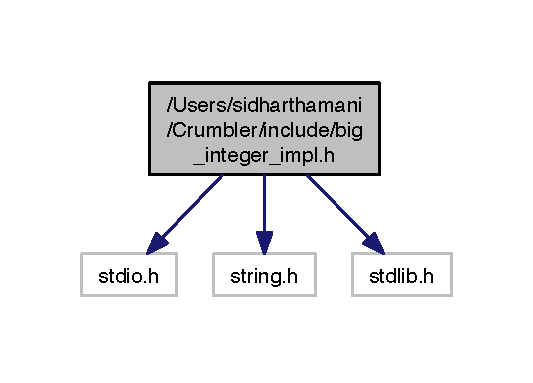
\includegraphics[width=256pt]{big__integer__impl_8h__incl}
\end{center}
\end{figure}
This graph shows which files directly or indirectly include this file\-:\nopagebreak
\begin{figure}[H]
\begin{center}
\leavevmode
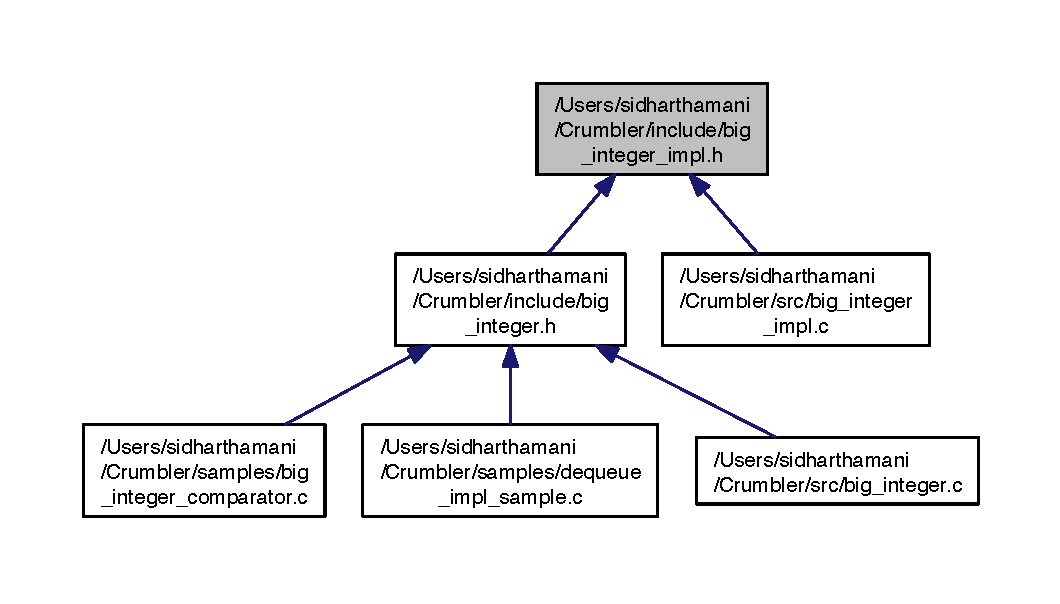
\includegraphics[width=350pt]{big__integer__impl_8h__dep__incl}
\end{center}
\end{figure}
\subsection*{Data Structures}
\begin{DoxyCompactItemize}
\item 
struct \hyperlink{big__integer__impl_8h_structbig__integer}{big\-\_\-integer}
\begin{DoxyCompactList}\small\item\em a struct to hold big integer values  \hyperlink{big__integer__impl_8h_structbig__integer}{More...}\end{DoxyCompactList}\end{DoxyCompactItemize}
\subsection*{Functions}
\begin{DoxyCompactItemize}
\item 
\hyperlink{big__integer__impl_8h_structbig__integer}{big\-\_\-integer} $\ast$ \hyperlink{big__integer__impl_8h_ad427e9cea709aee7a823b0136216fbfc}{init\-\_\-big\-\_\-integer} ()
\begin{DoxyCompactList}\small\item\em allocates memory for a new \hyperlink{big__integer__impl_8h_structbig__integer}{big\-\_\-integer} structure and returns a pointer to the allocated memory \par
 {\bfseries  Precondition\-: } the variable capturing the returned value should not have already been allocated memory \par
 {\bfseries  Postcondition\-: } memory is allocated and returned to the calling environment \end{DoxyCompactList}\item 
\hyperlink{big__integer__impl_8h_structbig__integer}{big\-\_\-integer} $\ast$ \hyperlink{big__integer__impl_8h_aba2b222c87a6ad23da34a0c8000e2506}{init\-\_\-big\-\_\-integer\-\_\-from\-\_\-int} (int int\-\_\-value)
\begin{DoxyCompactList}\small\item\em allocates memory for a new \hyperlink{big__integer__impl_8h_structbig__integer}{big\-\_\-integer} structure and returns a pointer to the allocated memory and initializes it to the value in int\-\_\-value\par
 {\bfseries  Precondition\-: } the variable capturing the returned value should not have already been allocated memory \par
 {\bfseries  Postcondition\-: } memory is allocated and initialized before returning to the calling environment \end{DoxyCompactList}\item 
\hyperlink{big__integer__impl_8h_structbig__integer}{big\-\_\-integer} $\ast$ \hyperlink{big__integer__impl_8h_a1329d3ba57def63a30fa2244a547eb29}{init\-\_\-big\-\_\-integer\-\_\-from\-\_\-long} (long long long\-\_\-long\-\_\-value)
\begin{DoxyCompactList}\small\item\em allocates memory for a new \hyperlink{big__integer__impl_8h_structbig__integer}{big\-\_\-integer} structure and returns a pointer to the allocated memory and initializes it to the value in long\-\_\-long\-\_\-value\par
 {\bfseries  Precondition\-: } the variable capturing the returned value should not have already been allocated memory \par
 {\bfseries  Postcondition\-: } memory is allocated and initialized before returning to the calling environment \end{DoxyCompactList}\item 
\hyperlink{big__integer__impl_8h_structbig__integer}{big\-\_\-integer} $\ast$ \hyperlink{big__integer__impl_8h_a78fe148b385a4ccb53b8b6c9cac949cb}{init\-\_\-big\-\_\-integer\-\_\-from\-\_\-char} (char $\ast$char\-\_\-value)
\begin{DoxyCompactList}\small\item\em allocates memory for a new \hyperlink{big__integer__impl_8h_structbig__integer}{big\-\_\-integer} structure and returns a pointer to the allocated memory and initializes it to the value in value\par
 {\bfseries  Precondition\-: } the variable capturing the returned value should not have already been allocated memory \par
 {\bfseries  Postcondition\-: } memory is allocated and initialized before returning to the calling environment \end{DoxyCompactList}\item 
int \hyperlink{big__integer__impl_8h_a12e0894b8887892194604e1217fe2afd}{compare\-\_\-big\-\_\-integers} (struct \hyperlink{big__integer__impl_8h_structbig__integer}{big\-\_\-integer} $\ast$operand1, struct \hyperlink{big__integer__impl_8h_structbig__integer}{big\-\_\-integer} $\ast$operand2)
\begin{DoxyCompactList}\small\item\em compares any two big\-\_\-integer(s) \par
 {\bfseries  Precondition\-: } the numbers being compared should have their signs set to 1 or -\/1\par
 {\bfseries  Postcondition\-: }The comparison result is returned \end{DoxyCompactList}\item 
\hyperlink{big__integer__impl_8h_structbig__integer}{big\-\_\-integer} $\ast$ \hyperlink{big__integer__impl_8h_acaa9b81fceecc01e260e7011fda3d628}{add\-\_\-big\-\_\-integers} (struct \hyperlink{big__integer__impl_8h_structbig__integer}{big\-\_\-integer} $\ast$operand1, struct \hyperlink{big__integer__impl_8h_structbig__integer}{big\-\_\-integer} $\ast$operand2, struct \hyperlink{big__integer__impl_8h_structbig__integer}{big\-\_\-integer} $\ast$result)
\begin{DoxyCompactList}\small\item\em adds two positive integers only\par
 {\bfseries  Postcondition\-: }the \hyperlink{big__integer__impl_8h_structbig__integer}{big\-\_\-integer} object containing the sum is returned \end{DoxyCompactList}\item 
void \hyperlink{big__integer__impl_8h_aba3732c4704a6c73493683133fcd9cae}{destroy\-\_\-big\-\_\-integer} (\hyperlink{big__integer__impl_8h_structbig__integer}{big\-\_\-integer} $\ast$obj)
\begin{DoxyCompactList}\small\item\em frees the allocated memory \par
 {\bfseries  Precondition\-: } the \hyperlink{big__integer__impl_8h_structbig__integer}{big\-\_\-integer} pointer which is being freed should not have been freed already \par
 {\bfseries  Postcondition\-: }The \hyperlink{big__integer__impl_8h_structbig__integer}{big\-\_\-integer} structure is freed \end{DoxyCompactList}\end{DoxyCompactItemize}


\subsection{Detailed Description}
The interface to the implementation of \hyperlink{big__integer__impl_8h_structbig__integer}{big\-\_\-integer} logic This file contains functions required to support the big integer manipulation functions.\par
 Author \-: Sidhartha Mani\par
 Contact \-: \href{mailto:sidharthamn@gmail.com}{\tt sidharthamn@gmail.\-com} \par
 Last Updated \-: 24 Dec 2012 \par
 

Definition in file \hyperlink{}{big\-\_\-integer\-\_\-impl.\-h}.



\subsection{Data Structure Documentation}
\index{big\-\_\-integer@{big\-\_\-integer}}\label{structbig__integer}
\hypertarget{big__integer__impl_8h_structbig__integer}{}
\subsubsection{struct big\-\_\-integer}
a struct to hold big integer values 

Definition at line 21 of file big\-\_\-integer\-\_\-impl.\-h.

\begin{DoxyFields}{Data Fields}
\hypertarget{big__integer__impl_8h_abbeb8ae63622a7fef0b5a56bb91a1682}{int}\label{big__integer__impl_8h_abbeb8ae63622a7fef0b5a56bb91a1682}
&
sign&
the sign of the integer \\
\hline

\hypertarget{big__integer__impl_8h_a4e9aec275e566b978a3ccb4e043d8c61}{char $\ast$}\label{big__integer__impl_8h_a4e9aec275e566b978a3ccb4e043d8c61}
&
value&
the string containing the \hyperlink{big__integer__impl_8h_structbig__integer}{big\-\_\-integer} \\
\hline

\end{DoxyFields}


\subsection{Function Documentation}
\hypertarget{big__integer__impl_8h_acaa9b81fceecc01e260e7011fda3d628}{\index{big\-\_\-integer\-\_\-impl.\-h@{big\-\_\-integer\-\_\-impl.\-h}!add\-\_\-big\-\_\-integers@{add\-\_\-big\-\_\-integers}}
\index{add\-\_\-big\-\_\-integers@{add\-\_\-big\-\_\-integers}!big_integer_impl.h@{big\-\_\-integer\-\_\-impl.\-h}}
\subsubsection[{add\-\_\-big\-\_\-integers}]{\setlength{\rightskip}{0pt plus 5cm}{\bf big\-\_\-integer} $\ast$ add\-\_\-big\-\_\-integers (
\begin{DoxyParamCaption}
\item[{struct {\bf big\-\_\-integer} $\ast$}]{operand1, }
\item[{struct {\bf big\-\_\-integer} $\ast$}]{operand2, }
\item[{struct {\bf big\-\_\-integer} $\ast$}]{result}
\end{DoxyParamCaption}
)}}\label{big__integer__impl_8h_acaa9b81fceecc01e260e7011fda3d628}


adds two positive integers only\par
 {\bfseries  Postcondition\-: }the \hyperlink{big__integer__impl_8h_structbig__integer}{big\-\_\-integer} object containing the sum is returned 


\begin{DoxyParams}{Parameters}
{\em operand1} & the first \hyperlink{big__integer__impl_8h_structbig__integer}{big\-\_\-integer} operand for addition \\
\hline
{\em operand2} & the second \hyperlink{big__integer__impl_8h_structbig__integer}{big\-\_\-integer} operand for addition \\
\hline
{\em result} & the \hyperlink{big__integer__impl_8h_structbig__integer}{big\-\_\-integer} structure in which the result should be stored, its ok if it was previously initialized or not \\
\hline
\end{DoxyParams}
\begin{DoxyReturn}{Returns}
a pointer to the \hyperlink{big__integer__impl_8h_structbig__integer}{big\-\_\-integer} holding the sum 
\end{DoxyReturn}


Definition at line 184 of file big\-\_\-integer\-\_\-impl.\-c.


\begin{DoxyCode}
\{
    \textcolor{keywordtype}{int} larger=(\hyperlink{big__integer__impl_8h_a12e0894b8887892194604e1217fe2afd}{compare\_big\_integers}(operand1,operand2)>=0)
      ?1:2;
    \textcolor{keywordtype}{char} new\_value[larger==1?strlen(operand1->\hyperlink{big__integer__impl_8h_a4e9aec275e566b978a3ccb4e043d8c61}{value})+2:strlen(operand2->
      \hyperlink{big__integer__impl_8h_a4e9aec275e566b978a3ccb4e043d8c61}{value})+2];
    new\_value[0] = \textcolor{charliteral}{'0'};
    new\_value[\textcolor{keyword}{sizeof}(new\_value) - 1] = \textcolor{charliteral}{'\(\backslash\)0'};
    \textcolor{keyword}{struct }\hyperlink{big__integer__impl_8h_structbig__integer}{big\_integer} *larger\_integer = (larger==1?operand1:
      operand2);  
    \textcolor{keyword}{struct }\hyperlink{big__integer__impl_8h_structbig__integer}{big\_integer} *shorter\_integer = (larger==2?operand1:
      operand2);
    \textcolor{keywordtype}{int} i = strlen(larger\_integer->\hyperlink{big__integer__impl_8h_a4e9aec275e566b978a3ccb4e043d8c61}{value});
    \textcolor{keywordtype}{int} j = strlen(shorter\_integer->\hyperlink{big__integer__impl_8h_a4e9aec275e566b978a3ccb4e043d8c61}{value}) - 1;
    \textcolor{keywordtype}{int} k = strlen(larger\_integer->\hyperlink{big__integer__impl_8h_a4e9aec275e566b978a3ccb4e043d8c61}{value});
    \textcolor{keywordtype}{int} sum;
    \textcolor{keywordtype}{int} carry = 0;
    \textcolor{keywordtype}{char} *new\_new\_value;
    \textcolor{keywordflow}{while} (i--) 
    \{
        \textcolor{keywordflow}{if} (j>=0)
        sum = ((int)larger\_integer->\hyperlink{big__integer__impl_8h_a4e9aec275e566b978a3ccb4e043d8c61}{value}[i] - (\textcolor{keywordtype}{int})\textcolor{charliteral}{'0'}) + ((\textcolor{keywordtype}{int})
      shorter\_integer->\hyperlink{big__integer__impl_8h_a4e9aec275e566b978a3ccb4e043d8c61}{value}[j--] - (int)\textcolor{charliteral}{'0'})+ carry;
        \textcolor{keywordflow}{else}
        sum = ((int)larger\_integer->\hyperlink{big__integer__impl_8h_a4e9aec275e566b978a3ccb4e043d8c61}{value}[i] - (\textcolor{keywordtype}{int})\textcolor{charliteral}{'0'}) + carry;
        carry = sum/10;
        sum = sum%10;
        new\_value[k--] = (char)(sum + \textcolor{charliteral}{'0'});
    \}
    \textcolor{keywordflow}{if} (carry != 0)
    \{
        new\_value[k] = carry;
        new\_new\_value = (\textcolor{keywordtype}{char} *)malloc((\textcolor{keywordtype}{int})strlen(new\_value));
        memcpy(new\_new\_value,new\_value,(\textcolor{keywordtype}{int})strlen(new\_value));
    \}
    \textcolor{keywordflow}{else} 
    \{
        new\_new\_value = (\textcolor{keywordtype}{char} *)malloc((\textcolor{keywordtype}{int})strlen(new\_value) - 1);
        memcpy(new\_new\_value,new\_value+1,(\textcolor{keywordtype}{int})strlen(new\_value)-1);
    \}
    \textcolor{keyword}{struct }\hyperlink{big__integer__impl_8h_structbig__integer}{big\_integer} *temp = \hyperlink{big__integer__impl_8h_a78fe148b385a4ccb53b8b6c9cac949cb}{init\_big\_integer\_from\_char}
      (new\_new\_value);
    temp->\hyperlink{big__integer__impl_8h_abbeb8ae63622a7fef0b5a56bb91a1682}{sign} = 1;
    \textcolor{keywordflow}{if}(result->\hyperlink{big__integer__impl_8h_a4e9aec275e566b978a3ccb4e043d8c61}{value} != NULL)
        \hyperlink{big__integer__impl_8h_aba3732c4704a6c73493683133fcd9cae}{destroy\_big\_integer}(result);
    result = temp;
    \textcolor{keywordflow}{return} result;
\}
\end{DoxyCode}
\hypertarget{big__integer__impl_8h_a12e0894b8887892194604e1217fe2afd}{\index{big\-\_\-integer\-\_\-impl.\-h@{big\-\_\-integer\-\_\-impl.\-h}!compare\-\_\-big\-\_\-integers@{compare\-\_\-big\-\_\-integers}}
\index{compare\-\_\-big\-\_\-integers@{compare\-\_\-big\-\_\-integers}!big_integer_impl.h@{big\-\_\-integer\-\_\-impl.\-h}}
\subsubsection[{compare\-\_\-big\-\_\-integers}]{\setlength{\rightskip}{0pt plus 5cm}int compare\-\_\-big\-\_\-integers (
\begin{DoxyParamCaption}
\item[{struct {\bf big\-\_\-integer} $\ast$}]{operand1, }
\item[{struct {\bf big\-\_\-integer} $\ast$}]{operand2}
\end{DoxyParamCaption}
)}}\label{big__integer__impl_8h_a12e0894b8887892194604e1217fe2afd}


compares any two big\-\_\-integer(s) \par
 {\bfseries  Precondition\-: } the numbers being compared should have their signs set to 1 or -\/1\par
 {\bfseries  Postcondition\-: }The comparison result is returned 


\begin{DoxyParams}{Parameters}
{\em operand1} & the operand against which the other operand will be compared \\
\hline
{\em operand2} & the operand which will be compared against operand1 \\
\hline
\end{DoxyParams}
\begin{DoxyReturn}{Returns}
\par
 Returns 0 \-: if both numbers are equal \par
 Returns $>$ 0 \-: if first value is larger \par
 Returns $<$ 0 \-: if first value is smaller 
\end{DoxyReturn}


Definition at line 142 of file big\-\_\-integer\-\_\-impl.\-c.


\begin{DoxyCode}
\{
    \textcolor{keywordflow}{if} (operand1->\hyperlink{big__integer__impl_8h_abbeb8ae63622a7fef0b5a56bb91a1682}{sign} == 1 && operand2->\hyperlink{big__integer__impl_8h_abbeb8ae63622a7fef0b5a56bb91a1682}{sign} == 1) 
    \{
        \textcolor{keywordflow}{if}(strlen(operand1->\hyperlink{big__integer__impl_8h_a4e9aec275e566b978a3ccb4e043d8c61}{value}) != strlen(operand2->\hyperlink{big__integer__impl_8h_a4e9aec275e566b978a3ccb4e043d8c61}{value}))
        \{
            \textcolor{keywordflow}{return} (strlen(operand1->\hyperlink{big__integer__impl_8h_a4e9aec275e566b978a3ccb4e043d8c61}{value})>strlen(operand2->\hyperlink{big__integer__impl_8h_a4e9aec275e566b978a3ccb4e043d8c61}{value})?1
      :-1);
        \}
        \textcolor{keywordflow}{return} strcmp(operand1->\hyperlink{big__integer__impl_8h_a4e9aec275e566b978a3ccb4e043d8c61}{value},operand2->\hyperlink{big__integer__impl_8h_a4e9aec275e566b978a3ccb4e043d8c61}{value});
    \}
    \textcolor{keywordflow}{else} \textcolor{keywordflow}{if}(operand1->\hyperlink{big__integer__impl_8h_abbeb8ae63622a7fef0b5a56bb91a1682}{sign} == -1 && operand2->\hyperlink{big__integer__impl_8h_abbeb8ae63622a7fef0b5a56bb91a1682}{sign} == -1)
    \{
        \textcolor{keywordflow}{if}(strlen(operand1->\hyperlink{big__integer__impl_8h_a4e9aec275e566b978a3ccb4e043d8c61}{value}) != strlen(operand2->\hyperlink{big__integer__impl_8h_a4e9aec275e566b978a3ccb4e043d8c61}{value}))
        \{
            \textcolor{keywordflow}{return} (strlen(operand1->\hyperlink{big__integer__impl_8h_a4e9aec275e566b978a3ccb4e043d8c61}{value})>strlen(operand2->\hyperlink{big__integer__impl_8h_a4e9aec275e566b978a3ccb4e043d8c61}{value})?-
      1:1);
        \}
        \textcolor{keywordflow}{return} strcmp(operand2->\hyperlink{big__integer__impl_8h_a4e9aec275e566b978a3ccb4e043d8c61}{value},operand1->\hyperlink{big__integer__impl_8h_a4e9aec275e566b978a3ccb4e043d8c61}{value});
    \}
    \textcolor{keywordflow}{return} (operand1->\hyperlink{big__integer__impl_8h_abbeb8ae63622a7fef0b5a56bb91a1682}{sign} == 1)?1:-1;
\}
\end{DoxyCode}
\hypertarget{big__integer__impl_8h_aba3732c4704a6c73493683133fcd9cae}{\index{big\-\_\-integer\-\_\-impl.\-h@{big\-\_\-integer\-\_\-impl.\-h}!destroy\-\_\-big\-\_\-integer@{destroy\-\_\-big\-\_\-integer}}
\index{destroy\-\_\-big\-\_\-integer@{destroy\-\_\-big\-\_\-integer}!big_integer_impl.h@{big\-\_\-integer\-\_\-impl.\-h}}
\subsubsection[{destroy\-\_\-big\-\_\-integer}]{\setlength{\rightskip}{0pt plus 5cm}void destroy\-\_\-big\-\_\-integer (
\begin{DoxyParamCaption}
\item[{{\bf big\-\_\-integer} $\ast$}]{obj}
\end{DoxyParamCaption}
)}}\label{big__integer__impl_8h_aba3732c4704a6c73493683133fcd9cae}


frees the allocated memory \par
 {\bfseries  Precondition\-: } the \hyperlink{big__integer__impl_8h_structbig__integer}{big\-\_\-integer} pointer which is being freed should not have been freed already \par
 {\bfseries  Postcondition\-: }The \hyperlink{big__integer__impl_8h_structbig__integer}{big\-\_\-integer} structure is freed 


\begin{DoxyParams}{Parameters}
{\em operand1} & the pointer to the structure which should be freed \\
\hline
\end{DoxyParams}
\begin{DoxyReturn}{Returns}
Nothing 
\end{DoxyReturn}


Definition at line 170 of file big\-\_\-integer\-\_\-impl.\-c.


\begin{DoxyCode}
\{
    free(obj->\hyperlink{big__integer__impl_8h_a4e9aec275e566b978a3ccb4e043d8c61}{value});
    free(obj);
\}
\end{DoxyCode}
\hypertarget{big__integer__impl_8h_ad427e9cea709aee7a823b0136216fbfc}{\index{big\-\_\-integer\-\_\-impl.\-h@{big\-\_\-integer\-\_\-impl.\-h}!init\-\_\-big\-\_\-integer@{init\-\_\-big\-\_\-integer}}
\index{init\-\_\-big\-\_\-integer@{init\-\_\-big\-\_\-integer}!big_integer_impl.h@{big\-\_\-integer\-\_\-impl.\-h}}
\subsubsection[{init\-\_\-big\-\_\-integer}]{\setlength{\rightskip}{0pt plus 5cm}{\bf big\-\_\-integer} $\ast$ init\-\_\-big\-\_\-integer (
\begin{DoxyParamCaption}
{}
\end{DoxyParamCaption}
)}}\label{big__integer__impl_8h_ad427e9cea709aee7a823b0136216fbfc}


allocates memory for a new \hyperlink{big__integer__impl_8h_structbig__integer}{big\-\_\-integer} structure and returns a pointer to the allocated memory \par
 {\bfseries  Precondition\-: } the variable capturing the returned value should not have already been allocated memory \par
 {\bfseries  Postcondition\-: } memory is allocated and returned to the calling environment 

\begin{DoxyReturn}{Returns}
a pointer to the allocated memory 
\end{DoxyReturn}


Definition at line 60 of file big\-\_\-integer\-\_\-impl.\-c.


\begin{DoxyCode}
\{
    \textcolor{keyword}{struct }\hyperlink{big__integer__impl_8h_structbig__integer}{big\_integer} *temp = (\textcolor{keyword}{struct }\hyperlink{big__integer__impl_8h_structbig__integer}{big\_integer}*)
      malloc(\textcolor{keyword}{sizeof}(\textcolor{keyword}{struct} \hyperlink{big__integer__impl_8h_structbig__integer}{big\_integer}));
    temp->\hyperlink{big__integer__impl_8h_a4e9aec275e566b978a3ccb4e043d8c61}{value} = NULL;
    temp->\hyperlink{big__integer__impl_8h_abbeb8ae63622a7fef0b5a56bb91a1682}{sign} = 1;
    \textcolor{keywordflow}{return} temp;
\}
\end{DoxyCode}
\hypertarget{big__integer__impl_8h_a78fe148b385a4ccb53b8b6c9cac949cb}{\index{big\-\_\-integer\-\_\-impl.\-h@{big\-\_\-integer\-\_\-impl.\-h}!init\-\_\-big\-\_\-integer\-\_\-from\-\_\-char@{init\-\_\-big\-\_\-integer\-\_\-from\-\_\-char}}
\index{init\-\_\-big\-\_\-integer\-\_\-from\-\_\-char@{init\-\_\-big\-\_\-integer\-\_\-from\-\_\-char}!big_integer_impl.h@{big\-\_\-integer\-\_\-impl.\-h}}
\subsubsection[{init\-\_\-big\-\_\-integer\-\_\-from\-\_\-char}]{\setlength{\rightskip}{0pt plus 5cm}{\bf big\-\_\-integer} $\ast$ init\-\_\-big\-\_\-integer\-\_\-from\-\_\-char (
\begin{DoxyParamCaption}
\item[{char $\ast$}]{value}
\end{DoxyParamCaption}
)}}\label{big__integer__impl_8h_a78fe148b385a4ccb53b8b6c9cac949cb}


allocates memory for a new \hyperlink{big__integer__impl_8h_structbig__integer}{big\-\_\-integer} structure and returns a pointer to the allocated memory and initializes it to the value in value\par
 {\bfseries  Precondition\-: } the variable capturing the returned value should not have already been allocated memory \par
 {\bfseries  Postcondition\-: } memory is allocated and initialized before returning to the calling environment 


\begin{DoxyParams}{Parameters}
{\em value} & the value, that will be converted into big integer representation \\
\hline
\end{DoxyParams}
\begin{DoxyReturn}{Returns}
a pointer to the allocated and initialized memory 
\end{DoxyReturn}


Definition at line 105 of file big\-\_\-integer\-\_\-impl.\-c.


\begin{DoxyCode}
\{
    \textcolor{keywordtype}{int} i = strlen(\hyperlink{big__integer__impl_8h_a4e9aec275e566b978a3ccb4e043d8c61}{value});
    \textcolor{comment}{//check for non-numbers}
    \textcolor{keywordflow}{while} (i--) \{
        \textcolor{keywordflow}{if}(!((\hyperlink{big__integer__impl_8h_a4e9aec275e566b978a3ccb4e043d8c61}{value}[i] <= \textcolor{charliteral}{'9'} && \hyperlink{big__integer__impl_8h_a4e9aec275e566b978a3ccb4e043d8c61}{value}[i] >= \textcolor{charliteral}{'0'}) || (i==0 && \hyperlink{big__integer__impl_8h_a4e9aec275e566b978a3ccb4e043d8c61}{value}
      [i] == \textcolor{charliteral}{'-'})))
            \textcolor{keywordflow}{return} NULL;
    \}
    \textcolor{comment}{//check for preceeding 0's}
    i++;
    \textcolor{keywordflow}{while} (i<strlen(\hyperlink{big__integer__impl_8h_a4e9aec275e566b978a3ccb4e043d8c61}{value}) && \hyperlink{big__integer__impl_8h_a4e9aec275e566b978a3ccb4e043d8c61}{value}[i++] == \textcolor{charliteral}{'0'});
    i--;
    \textcolor{keywordtype}{char} *new\_value = (\textcolor{keywordtype}{char}*)malloc(strlen(\hyperlink{big__integer__impl_8h_a4e9aec275e566b978a3ccb4e043d8c61}{value}));
    \textcolor{keywordflow}{if}(i != strlen(\hyperlink{big__integer__impl_8h_a4e9aec275e566b978a3ccb4e043d8c61}{value}))
    \{
        memcpy(new\_value,\hyperlink{big__integer__impl_8h_a4e9aec275e566b978a3ccb4e043d8c61}{value} + i,(\textcolor{keywordtype}{int})strlen(\hyperlink{big__integer__impl_8h_a4e9aec275e566b978a3ccb4e043d8c61}{value}) - i);
    \}   
    \textcolor{keywordflow}{else} 
    \{
        memcpy(new\_value,\textcolor{stringliteral}{"0"},1);
    \}
    \textcolor{keyword}{struct }\hyperlink{big__integer__impl_8h_structbig__integer}{big\_integer} *temp = \hyperlink{big__integer__impl_8h_ad427e9cea709aee7a823b0136216fbfc}{init\_big\_integer}();
    ((\hyperlink{big__integer__impl_8h_a4e9aec275e566b978a3ccb4e043d8c61}{value}[0] == \textcolor{charliteral}{'-'})?(temp->\hyperlink{big__integer__impl_8h_a4e9aec275e566b978a3ccb4e043d8c61}{value}=new\_value+1,temp->\hyperlink{big__integer__impl_8h_abbeb8ae63622a7fef0b5a56bb91a1682}{sign} = -1):
      (temp->\hyperlink{big__integer__impl_8h_a4e9aec275e566b978a3ccb4e043d8c61}{value} = new\_value,temp->\hyperlink{big__integer__impl_8h_abbeb8ae63622a7fef0b5a56bb91a1682}{sign} = 1));
    \textcolor{keywordflow}{return} temp;
\}
\end{DoxyCode}
\hypertarget{big__integer__impl_8h_aba2b222c87a6ad23da34a0c8000e2506}{\index{big\-\_\-integer\-\_\-impl.\-h@{big\-\_\-integer\-\_\-impl.\-h}!init\-\_\-big\-\_\-integer\-\_\-from\-\_\-int@{init\-\_\-big\-\_\-integer\-\_\-from\-\_\-int}}
\index{init\-\_\-big\-\_\-integer\-\_\-from\-\_\-int@{init\-\_\-big\-\_\-integer\-\_\-from\-\_\-int}!big_integer_impl.h@{big\-\_\-integer\-\_\-impl.\-h}}
\subsubsection[{init\-\_\-big\-\_\-integer\-\_\-from\-\_\-int}]{\setlength{\rightskip}{0pt plus 5cm}{\bf big\-\_\-integer} $\ast$ init\-\_\-big\-\_\-integer\-\_\-from\-\_\-int (
\begin{DoxyParamCaption}
\item[{int}]{int\-\_\-value}
\end{DoxyParamCaption}
)}}\label{big__integer__impl_8h_aba2b222c87a6ad23da34a0c8000e2506}


allocates memory for a new \hyperlink{big__integer__impl_8h_structbig__integer}{big\-\_\-integer} structure and returns a pointer to the allocated memory and initializes it to the value in int\-\_\-value\par
 {\bfseries  Precondition\-: } the variable capturing the returned value should not have already been allocated memory \par
 {\bfseries  Postcondition\-: } memory is allocated and initialized before returning to the calling environment 


\begin{DoxyParams}{Parameters}
{\em int\-\_\-value} & the long int value, that will be converted into big integer representation \\
\hline
\end{DoxyParams}
\begin{DoxyReturn}{Returns}
a pointer to the allocated and initialized memory 
\end{DoxyReturn}


Definition at line 92 of file big\-\_\-integer\-\_\-impl.\-c.


\begin{DoxyCode}
\{
    \textcolor{keywordflow}{return} \hyperlink{big__integer__impl_8h_a1329d3ba57def63a30fa2244a547eb29}{init\_big\_integer\_from\_long}((\textcolor{keywordtype}{long} \textcolor{keywordtype}{long})
      int\_value);
\}
\end{DoxyCode}
\hypertarget{big__integer__impl_8h_a1329d3ba57def63a30fa2244a547eb29}{\index{big\-\_\-integer\-\_\-impl.\-h@{big\-\_\-integer\-\_\-impl.\-h}!init\-\_\-big\-\_\-integer\-\_\-from\-\_\-long@{init\-\_\-big\-\_\-integer\-\_\-from\-\_\-long}}
\index{init\-\_\-big\-\_\-integer\-\_\-from\-\_\-long@{init\-\_\-big\-\_\-integer\-\_\-from\-\_\-long}!big_integer_impl.h@{big\-\_\-integer\-\_\-impl.\-h}}
\subsubsection[{init\-\_\-big\-\_\-integer\-\_\-from\-\_\-long}]{\setlength{\rightskip}{0pt plus 5cm}{\bf big\-\_\-integer} $\ast$ init\-\_\-big\-\_\-integer\-\_\-from\-\_\-long (
\begin{DoxyParamCaption}
\item[{long long}]{long\-\_\-long\-\_\-value}
\end{DoxyParamCaption}
)}}\label{big__integer__impl_8h_a1329d3ba57def63a30fa2244a547eb29}


allocates memory for a new \hyperlink{big__integer__impl_8h_structbig__integer}{big\-\_\-integer} structure and returns a pointer to the allocated memory and initializes it to the value in long\-\_\-long\-\_\-value\par
 {\bfseries  Precondition\-: } the variable capturing the returned value should not have already been allocated memory \par
 {\bfseries  Postcondition\-: } memory is allocated and initialized before returning to the calling environment 


\begin{DoxyParams}{Parameters}
{\em long\-\_\-long\-\_\-value} & the long long value, that will be converted into big integer representation \\
\hline
\end{DoxyParams}
\begin{DoxyReturn}{Returns}
a pointer to the allocated and initialized memory 
\end{DoxyReturn}


Definition at line 76 of file big\-\_\-integer\-\_\-impl.\-c.


\begin{DoxyCode}
\{
    \textcolor{keyword}{struct }\hyperlink{big__integer__impl_8h_structbig__integer}{big\_integer} *temp = \hyperlink{big__integer__impl_8h_ad427e9cea709aee7a823b0136216fbfc}{init\_big\_integer}();
    temp->\hyperlink{big__integer__impl_8h_a4e9aec275e566b978a3ccb4e043d8c61}{value} = \hyperlink{big__integer__impl_8c_ac9b89d7643e2d33ff43b6b19cf8e626c}{long\_long\_to\_char}(long\_long\_value);
    temp->\hyperlink{big__integer__impl_8h_abbeb8ae63622a7fef0b5a56bb91a1682}{sign} = ((long\_long\_value<0)?-1:1);
    \textcolor{keywordflow}{return} temp;
\}
\end{DoxyCode}

\hypertarget{simple__prefix_8h}{\section{/\-Users/sidharthamani/huffman\-\_\-coder/include/simple\-\_\-prefix.h File Reference}
\label{simple__prefix_8h}\index{/\-Users/sidharthamani/huffman\-\_\-coder/include/simple\-\_\-prefix.\-h@{/\-Users/sidharthamani/huffman\-\_\-coder/include/simple\-\_\-prefix.\-h}}
}
{\ttfamily \#include \char`\"{}simple\-\_\-prefix\-\_\-impl.\-h\char`\"{}}\\*
Include dependency graph for simple\-\_\-prefix.\-h\-:
This graph shows which files directly or indirectly include this file\-:
\subsection*{Data Structures}
\begin{DoxyCompactItemize}
\item 
struct \hyperlink{structsimple__prefix}{simple\-\_\-prefix}
\end{DoxyCompactItemize}
\subsection*{Typedefs}
\begin{DoxyCompactItemize}
\item 
typedef struct \hyperlink{structsimple__prefix}{simple\-\_\-prefix} \hyperlink{simple__prefix_8h_a7d6089974f5d15d068518c5de7c9d1b7}{simple\-\_\-prefix}
\end{DoxyCompactItemize}
\subsection*{Functions}
\begin{DoxyCompactItemize}
\item 
\hyperlink{structsimple__prefix}{simple\-\_\-prefix} $\ast$ \hyperlink{simple__prefix_8h_a9bd5b14908a928a995ad497e7d037394}{init} ()
\end{DoxyCompactItemize}


\subsection{Typedef Documentation}
\hypertarget{simple__prefix_8h_a7d6089974f5d15d068518c5de7c9d1b7}{\index{simple\-\_\-prefix.\-h@{simple\-\_\-prefix.\-h}!simple\-\_\-prefix@{simple\-\_\-prefix}}
\index{simple\-\_\-prefix@{simple\-\_\-prefix}!simple_prefix.h@{simple\-\_\-prefix.\-h}}
\subsubsection[{simple\-\_\-prefix}]{\setlength{\rightskip}{0pt plus 5cm}typedef struct {\bf simple\-\_\-prefix} {\bf simple\-\_\-prefix}}}\label{simple__prefix_8h_a7d6089974f5d15d068518c5de7c9d1b7}


\subsection{Function Documentation}
\hypertarget{simple__prefix_8h_a9bd5b14908a928a995ad497e7d037394}{\index{simple\-\_\-prefix.\-h@{simple\-\_\-prefix.\-h}!init@{init}}
\index{init@{init}!simple_prefix.h@{simple\-\_\-prefix.\-h}}
\subsubsection[{init}]{\setlength{\rightskip}{0pt plus 5cm}{\bf simple\-\_\-prefix}$\ast$ init (
\begin{DoxyParamCaption}
{}
\end{DoxyParamCaption}
)}}\label{simple__prefix_8h_a9bd5b14908a928a995ad497e7d037394}

\begin{DoxyCode}
\{
    \textcolor{keyword}{struct }\hyperlink{structsimple__prefix}{simple\_prefix} *x\_simple\_prefix = (\textcolor{keyword}{struct }\hyperlink{structsimple__prefix}{simple\_prefix}
      *)malloc(\textcolor{keyword}{sizeof}(\hyperlink{structsimple__prefix}{simple\_prefix}));
    x\_simple\_prefix->\hyperlink{structsimple__prefix_a73d0a239981b130553964b3839c20bdf}{encode\_file} = \hyperlink{simple__prefix_8c_ac55c02996682de17f87b5c1116bb9944}{x\_encode\_file};
    x\_simple\_prefix->\hyperlink{structsimple__prefix_a58708e15f01f3be37e12d3194e953b41}{decode\_file} = \hyperlink{simple__prefix_8c_a1c9ef3bc94f0f14191b5956bb4040867}{x\_decode\_file};
    \textcolor{keywordflow}{return} x\_simple\_prefix;
\}\end{DoxyCode}

\hypertarget{simple__prefix__impl_8h}{\section{/\-Users/sidharthamani/\-Crumbler/include/simple\-\_\-prefix\-\_\-impl.h File Reference}
\label{simple__prefix__impl_8h}\index{/\-Users/sidharthamani/\-Crumbler/include/simple\-\_\-prefix\-\_\-impl.\-h@{/\-Users/sidharthamani/\-Crumbler/include/simple\-\_\-prefix\-\_\-impl.\-h}}
}


serves as the interface to the implementation of \hyperlink{structsimple__prefix}{simple\-\_\-prefix} tree This file contains functions required to support the encoding and de-\/coding functions.\par
 Author \-: Sidhartha Mani\par
 Contact \-: \href{mailto:sidharthamn@gmail.com}{\tt sidharthamn@gmail.\-com} \par
 Last Updated \-: 23 Dec 2012 \par
  


{\ttfamily \#include $<$stdio.\-h$>$}\\*
{\ttfamily \#include $<$stdlib.\-h$>$}\\*
{\ttfamily \#include $<$string.\-h$>$}\\*
Include dependency graph for simple\-\_\-prefix\-\_\-impl.\-h\-:\nopagebreak
\begin{figure}[H]
\begin{center}
\leavevmode
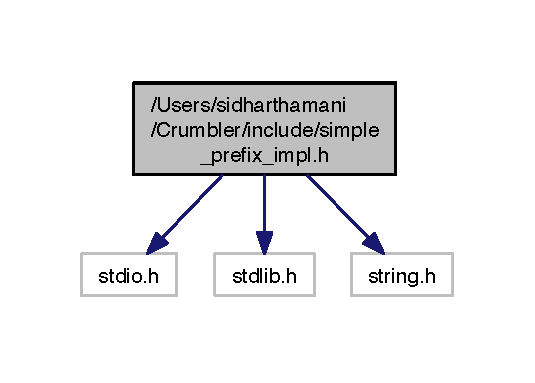
\includegraphics[width=257pt]{simple__prefix__impl_8h__incl}
\end{center}
\end{figure}
This graph shows which files directly or indirectly include this file\-:\nopagebreak
\begin{figure}[H]
\begin{center}
\leavevmode
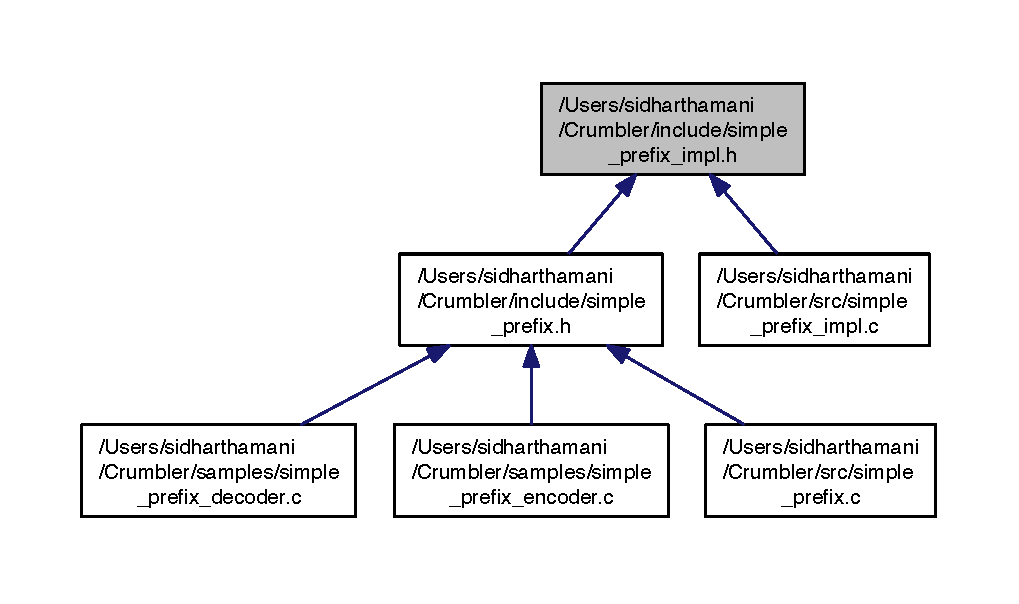
\includegraphics[width=350pt]{simple__prefix__impl_8h__dep__incl}
\end{center}
\end{figure}
\subsection*{Data Structures}
\begin{DoxyCompactItemize}
\item 
struct \hyperlink{simple__prefix__impl_8h_structnode}{node}
\begin{DoxyCompactList}\small\item\em a node of a \hyperlink{structsimple__prefix}{simple\-\_\-prefix} tree  \hyperlink{simple__prefix__impl_8h_structnode}{More...}\end{DoxyCompactList}\end{DoxyCompactItemize}
\subsection*{Macros}
\begin{DoxyCompactItemize}
\item 
\#define \hyperlink{simple__prefix__impl_8h_a94747a3d988297667d1f086be19a7f3d}{L\-O\-W\-E\-R\-\_\-\-C\-A\-S\-E\-\_\-\-A\-L\-P\-H\-A\-B\-E\-T\-S}~\char`\"{}eariotnslcudpmhgbfywkvxzjq \char`\"{}
\begin{DoxyCompactList}\small\item\em writing \hyperlink{structsimple__prefix}{simple\-\_\-prefix} codes only for lower case alphabets now, will write for the rest later The letters in the macro L\-O\-W\-E\-R\-\_\-\-C\-A\-S\-E\-\_\-\-A\-L\-P\-H\-A\-B\-E\-T\-S are sorted based on letters occuring with highest frequency in words from the oxford dictionary -\/ \href{http://oxforddictionaries.com/words/what-is-the-frequency-of-the-letters-of-the-alphabet-in-english}{\tt http\-://oxforddictionaries.\-com/words/what-\/is-\/the-\/frequency-\/of-\/the-\/letters-\/of-\/the-\/alphabet-\/in-\/english} \end{DoxyCompactList}\item 
\#define \hyperlink{simple__prefix__impl_8h_aa462b833c678d200d3a76f3dc16d415c}{U\-P\-P\-E\-R\-\_\-\-C\-A\-S\-E\-\_\-\-A\-L\-P\-H\-A\-B\-E\-T\-S}~\char`\"{}A\-B\-C\-D\-E\-F\-G\-H\-I\-J\-K\-L\-M\-N\-O\-P\-Q\-R\-S\-T\-U\-V\-W\-X\-Y\-Z\char`\"{}
\begin{DoxyCompactList}\small\item\em the list of upper case alphabets, to be used later \end{DoxyCompactList}\item 
\#define \hyperlink{simple__prefix__impl_8h_a52c6eed29863def7303121b65975e83b}{N\-U\-M\-B\-E\-R\-S}~\char`\"{}0123456789\char`\"{}
\begin{DoxyCompactList}\small\item\em the list of numbers, to be used later \end{DoxyCompactList}\item 
\#define \hyperlink{simple__prefix__impl_8h_aca3321d60a25310d108cb125e8e639e0}{W\-H\-I\-T\-E\-\_\-\-S\-P\-A\-C\-E}~\char`\"{} \char`\"{}
\begin{DoxyCompactList}\small\item\em white space character(depreceated). Already incorporated in L\-O\-W\-E\-R\-\_\-\-C\-A\-S\-E\-\_\-\-A\-L\-P\-H\-A\-B\-E\-T\-S \end{DoxyCompactList}\item 
\#define \hyperlink{simple__prefix__impl_8h_a7b99dc1e1c86b4897498c2d436ead1b5}{N\-E\-W\-\_\-\-L\-I\-N\-E}~\char`\"{}\textbackslash{}n\char`\"{}
\begin{DoxyCompactList}\small\item\em new line character, to be used later \end{DoxyCompactList}\item 
\#define \hyperlink{simple__prefix__impl_8h_af281425e62298bac2df0fbe8690a4844}{P\-E\-R\-I\-O\-D}~\char`\"{}.\char`\"{}
\begin{DoxyCompactList}\small\item\em period character, to be used later \end{DoxyCompactList}\item 
\#define \hyperlink{simple__prefix__impl_8h_aa2f49001be13949a16a57e6c99ab00ad}{C\-O\-M\-M\-A}~\char`\"{},\char`\"{}
\begin{DoxyCompactList}\small\item\em comma character, to be used later \end{DoxyCompactList}\end{DoxyCompactItemize}
\subsection*{Functions}
\begin{DoxyCompactItemize}
\item 
\hyperlink{simple__prefix__impl_8h_structnode}{node} $\ast$ \hyperlink{simple__prefix__impl_8h_af8da3d9dd76b4948b2233ed801729904}{init\-\_\-simple\-\_\-prefix} ()
\begin{DoxyCompactList}\small\item\em allocate memory for a new \hyperlink{structsimple__prefix}{simple\-\_\-prefix} tree \par
 {\bfseries Precondition\-:} The structure should not have already been allocated memory \par
 {\bfseries Postcondition\-:} Memory is allocated and returned to the calling environment \par
 \end{DoxyCompactList}\item 
\hyperlink{simple__prefix__impl_8h_structnode}{node} $\ast$ \hyperlink{simple__prefix__impl_8h_a2803bf8d5b507d080053c5795f1f2e8e}{construct\-\_\-simple\-\_\-prefix\-\_\-tree} (struct \hyperlink{simple__prefix__impl_8h_structnode}{node} $\ast$root, char $\ast$input\-\_\-msgs, int size\-\_\-of\-\_\-input\-\_\-msgs)
\begin{DoxyCompactList}\small\item\em construct a naive \hyperlink{structsimple__prefix}{simple\-\_\-prefix} tree for a set of characters specified by input\-\_\-msgs \par
 {\bfseries  Precondition\-: } Root should have already been initialized \par
 {\bfseries  Postcondition\-: } The Root is initialized to a simple prefix tree for all printable characters \par
 \end{DoxyCompactList}\item 
char $\ast$ \hyperlink{simple__prefix__impl_8h_a1d974ca63f3322d8a7d444c6ebbf6212}{simple\-\_\-prefix\-\_\-encode} (char $\ast$msg, int size\-\_\-of\-\_\-msg)
\begin{DoxyCompactList}\small\item\em encode a string based on the current \hyperlink{structsimple__prefix}{simple\-\_\-prefix} tree, size\-\_\-of\-\_\-msgs(param 2) should be specified in bytes\par
 {\bfseries Precondition \-:} The string into which the returned value should be captured should not have already been allocated. Right now, the function can only encode characters defined in L\-O\-W\-E\-R\-\_\-\-C\-A\-S\-E\-\_\-\-A\-L\-P\-H\-A\-B\-E\-T\-S macro\par
 {\bfseries Postcondition \-:} The message is encoded according to the \hyperlink{structsimple__prefix}{simple\-\_\-prefix} algorithm and returned to the calling environment \end{DoxyCompactList}\item 
char $\ast$ \hyperlink{simple__prefix__impl_8h_a01c7baaef3398c045f127558eeef0b14}{simple\-\_\-prefix\-\_\-decode} (char $\ast$encoded\-\_\-string, struct \hyperlink{simple__prefix__impl_8h_structnode}{node} $\ast$root, int size\-\_\-of\-\_\-encoded\-\_\-string)
\begin{DoxyCompactList}\small\item\em decode an encoded string by using the prefix tree generated by construct\-\_\-simple\-\_\-prefix(struct node$\ast$, char$\ast$, int) The parameter 2 (struct node$\ast$ root) is a pointer to the generated tree.\par
 {\bfseries Precondition \-:} The tree should have already been generated. The string capturing the return value should not have already been allocated memory\par
 {\bfseries Postcondition \-:} The encoded string is decoded and returned to the calling environment \end{DoxyCompactList}\item 
char $\ast$ \hyperlink{simple__prefix__impl_8h_ad1bc46a0b15e7c78972582382c673f67}{char2bits} (char $\ast$encoded\-\_\-string, int size\-\_\-of\-\_\-encoded\-\_\-string)
\begin{DoxyCompactList}\small\item\em convert encoded character array into bits for reducing storage space. Use this on an encoded string before persisting this in a file or wherever\par
 {\bfseries Precondition \-:} The string capturing the return value should not have already been allocated memory\par
 {\bfseries Postcondition \-:} The binary representation of the encoded string is returned as an array of bytes(char) \end{DoxyCompactList}\item 
char $\ast$ \hyperlink{simple__prefix__impl_8h_a8e5c5d48a1976c228264eed42c276209}{bits2char} (char $\ast$bit\-\_\-stream, int size\-\_\-of\-\_\-bit\-\_\-stream)
\begin{DoxyCompactList}\small\item\em convert encoded bits(as binary data) into a character array for decoding. Use this whenever you read from a persisted source.\-simple\-\_\-prefix\-\_\-decode(char$\ast$, struct node$\ast$, int) undersands encoded strings in char format, not actual binary. Lots of improvement required in this function. Right now, it can only work with the constraint of encoded string length being a multiple of 8.\par
 {\bfseries Precondition \-:} The string capturing the return value should not have already been allocated memory\par
 {\bfseries Postcondition \-:} The character representation of the encoded binary string is returned as an array of bytes(char) \end{DoxyCompactList}\end{DoxyCompactItemize}


\subsection{Detailed Description}
serves as the interface to the implementation of \hyperlink{structsimple__prefix}{simple\-\_\-prefix} tree This file contains functions required to support the encoding and de-\/coding functions.\par
 Author \-: Sidhartha Mani\par
 Contact \-: \href{mailto:sidharthamn@gmail.com}{\tt sidharthamn@gmail.\-com} \par
 Last Updated \-: 23 Dec 2012 \par
 

Definition in file \hyperlink{}{simple\-\_\-prefix\-\_\-impl.\-h}.



\subsection{Data Structure Documentation}
\index{node@{node}}\label{structnode}
\hypertarget{simple__prefix__impl_8h_structnode}{}
\subsubsection{struct node}
a node of a \hyperlink{structsimple__prefix}{simple\-\_\-prefix} tree 

Definition at line 66 of file simple\-\_\-prefix\-\_\-impl.\-h.



Collaboration diagram for node\-:\nopagebreak
\begin{figure}[H]
\begin{center}
\leavevmode
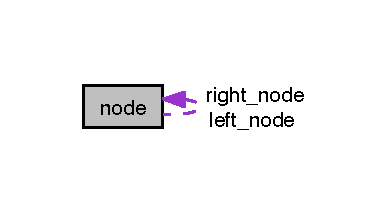
\includegraphics[width=186pt]{structnode__coll__graph}
\end{center}
\end{figure}
\begin{DoxyFields}{Data Fields}
\hypertarget{simple__prefix__impl_8h_ad066657fe1374fb9852c285175a3774f}{int}\label{simple__prefix__impl_8h_ad066657fe1374fb9852c285175a3774f}
&
is\-\_\-leaf&
Represents if the node is a leaf or not. If 0 it is not a leaf, If 1 it is a leaf \\
\hline

\hypertarget{simple__prefix__impl_8h_a43dd3cf499d5b2270fcfbb29eb0a0d66}{struct \hyperlink{simple__prefix__impl_8h_structnode}{node} $\ast$}\label{simple__prefix__impl_8h_a43dd3cf499d5b2270fcfbb29eb0a0d66}
&
left\-\_\-node&
The pointer to the left subtree \\
\hline

\hypertarget{simple__prefix__impl_8h_ad80e777cd260fdd5ca6ad3f25b5e76de}{char}\label{simple__prefix__impl_8h_ad80e777cd260fdd5ca6ad3f25b5e76de}
&
msg&
The character that a node encodes, is saved as a msg in this variable \\
\hline

\hypertarget{simple__prefix__impl_8h_af729d9e66cefdd8c0a114cb0da5f7b7c}{struct \hyperlink{simple__prefix__impl_8h_structnode}{node} $\ast$}\label{simple__prefix__impl_8h_af729d9e66cefdd8c0a114cb0da5f7b7c}
&
right\-\_\-node&
The pointer to the right subtree \\
\hline

\end{DoxyFields}


\subsection{Macro Definition Documentation}
\hypertarget{simple__prefix__impl_8h_aa2f49001be13949a16a57e6c99ab00ad}{\index{simple\-\_\-prefix\-\_\-impl.\-h@{simple\-\_\-prefix\-\_\-impl.\-h}!C\-O\-M\-M\-A@{C\-O\-M\-M\-A}}
\index{C\-O\-M\-M\-A@{C\-O\-M\-M\-A}!simple_prefix_impl.h@{simple\-\_\-prefix\-\_\-impl.\-h}}
\subsubsection[{C\-O\-M\-M\-A}]{\setlength{\rightskip}{0pt plus 5cm}\#define C\-O\-M\-M\-A~\char`\"{},\char`\"{}}}\label{simple__prefix__impl_8h_aa2f49001be13949a16a57e6c99ab00ad}


comma character, to be used later 



Definition at line 61 of file simple\-\_\-prefix\-\_\-impl.\-h.

\hypertarget{simple__prefix__impl_8h_a94747a3d988297667d1f086be19a7f3d}{\index{simple\-\_\-prefix\-\_\-impl.\-h@{simple\-\_\-prefix\-\_\-impl.\-h}!L\-O\-W\-E\-R\-\_\-\-C\-A\-S\-E\-\_\-\-A\-L\-P\-H\-A\-B\-E\-T\-S@{L\-O\-W\-E\-R\-\_\-\-C\-A\-S\-E\-\_\-\-A\-L\-P\-H\-A\-B\-E\-T\-S}}
\index{L\-O\-W\-E\-R\-\_\-\-C\-A\-S\-E\-\_\-\-A\-L\-P\-H\-A\-B\-E\-T\-S@{L\-O\-W\-E\-R\-\_\-\-C\-A\-S\-E\-\_\-\-A\-L\-P\-H\-A\-B\-E\-T\-S}!simple_prefix_impl.h@{simple\-\_\-prefix\-\_\-impl.\-h}}
\subsubsection[{L\-O\-W\-E\-R\-\_\-\-C\-A\-S\-E\-\_\-\-A\-L\-P\-H\-A\-B\-E\-T\-S}]{\setlength{\rightskip}{0pt plus 5cm}\#define L\-O\-W\-E\-R\-\_\-\-C\-A\-S\-E\-\_\-\-A\-L\-P\-H\-A\-B\-E\-T\-S~\char`\"{}eariotnslcudpmhgbfywkvxzjq \char`\"{}}}\label{simple__prefix__impl_8h_a94747a3d988297667d1f086be19a7f3d}


writing \hyperlink{structsimple__prefix}{simple\-\_\-prefix} codes only for lower case alphabets now, will write for the rest later The letters in the macro L\-O\-W\-E\-R\-\_\-\-C\-A\-S\-E\-\_\-\-A\-L\-P\-H\-A\-B\-E\-T\-S are sorted based on letters occuring with highest frequency in words from the oxford dictionary -\/ \href{http://oxforddictionaries.com/words/what-is-the-frequency-of-the-letters-of-the-alphabet-in-english}{\tt http\-://oxforddictionaries.\-com/words/what-\/is-\/the-\/frequency-\/of-\/the-\/letters-\/of-\/the-\/alphabet-\/in-\/english} 



Definition at line 31 of file simple\-\_\-prefix\-\_\-impl.\-h.

\hypertarget{simple__prefix__impl_8h_a7b99dc1e1c86b4897498c2d436ead1b5}{\index{simple\-\_\-prefix\-\_\-impl.\-h@{simple\-\_\-prefix\-\_\-impl.\-h}!N\-E\-W\-\_\-\-L\-I\-N\-E@{N\-E\-W\-\_\-\-L\-I\-N\-E}}
\index{N\-E\-W\-\_\-\-L\-I\-N\-E@{N\-E\-W\-\_\-\-L\-I\-N\-E}!simple_prefix_impl.h@{simple\-\_\-prefix\-\_\-impl.\-h}}
\subsubsection[{N\-E\-W\-\_\-\-L\-I\-N\-E}]{\setlength{\rightskip}{0pt plus 5cm}\#define N\-E\-W\-\_\-\-L\-I\-N\-E~\char`\"{}\textbackslash{}n\char`\"{}}}\label{simple__prefix__impl_8h_a7b99dc1e1c86b4897498c2d436ead1b5}


new line character, to be used later 



Definition at line 51 of file simple\-\_\-prefix\-\_\-impl.\-h.

\hypertarget{simple__prefix__impl_8h_a52c6eed29863def7303121b65975e83b}{\index{simple\-\_\-prefix\-\_\-impl.\-h@{simple\-\_\-prefix\-\_\-impl.\-h}!N\-U\-M\-B\-E\-R\-S@{N\-U\-M\-B\-E\-R\-S}}
\index{N\-U\-M\-B\-E\-R\-S@{N\-U\-M\-B\-E\-R\-S}!simple_prefix_impl.h@{simple\-\_\-prefix\-\_\-impl.\-h}}
\subsubsection[{N\-U\-M\-B\-E\-R\-S}]{\setlength{\rightskip}{0pt plus 5cm}\#define N\-U\-M\-B\-E\-R\-S~\char`\"{}0123456789\char`\"{}}}\label{simple__prefix__impl_8h_a52c6eed29863def7303121b65975e83b}


the list of numbers, to be used later 



Definition at line 41 of file simple\-\_\-prefix\-\_\-impl.\-h.

\hypertarget{simple__prefix__impl_8h_af281425e62298bac2df0fbe8690a4844}{\index{simple\-\_\-prefix\-\_\-impl.\-h@{simple\-\_\-prefix\-\_\-impl.\-h}!P\-E\-R\-I\-O\-D@{P\-E\-R\-I\-O\-D}}
\index{P\-E\-R\-I\-O\-D@{P\-E\-R\-I\-O\-D}!simple_prefix_impl.h@{simple\-\_\-prefix\-\_\-impl.\-h}}
\subsubsection[{P\-E\-R\-I\-O\-D}]{\setlength{\rightskip}{0pt plus 5cm}\#define P\-E\-R\-I\-O\-D~\char`\"{}.\char`\"{}}}\label{simple__prefix__impl_8h_af281425e62298bac2df0fbe8690a4844}


period character, to be used later 



Definition at line 56 of file simple\-\_\-prefix\-\_\-impl.\-h.

\hypertarget{simple__prefix__impl_8h_aa462b833c678d200d3a76f3dc16d415c}{\index{simple\-\_\-prefix\-\_\-impl.\-h@{simple\-\_\-prefix\-\_\-impl.\-h}!U\-P\-P\-E\-R\-\_\-\-C\-A\-S\-E\-\_\-\-A\-L\-P\-H\-A\-B\-E\-T\-S@{U\-P\-P\-E\-R\-\_\-\-C\-A\-S\-E\-\_\-\-A\-L\-P\-H\-A\-B\-E\-T\-S}}
\index{U\-P\-P\-E\-R\-\_\-\-C\-A\-S\-E\-\_\-\-A\-L\-P\-H\-A\-B\-E\-T\-S@{U\-P\-P\-E\-R\-\_\-\-C\-A\-S\-E\-\_\-\-A\-L\-P\-H\-A\-B\-E\-T\-S}!simple_prefix_impl.h@{simple\-\_\-prefix\-\_\-impl.\-h}}
\subsubsection[{U\-P\-P\-E\-R\-\_\-\-C\-A\-S\-E\-\_\-\-A\-L\-P\-H\-A\-B\-E\-T\-S}]{\setlength{\rightskip}{0pt plus 5cm}\#define U\-P\-P\-E\-R\-\_\-\-C\-A\-S\-E\-\_\-\-A\-L\-P\-H\-A\-B\-E\-T\-S~\char`\"{}A\-B\-C\-D\-E\-F\-G\-H\-I\-J\-K\-L\-M\-N\-O\-P\-Q\-R\-S\-T\-U\-V\-W\-X\-Y\-Z\char`\"{}}}\label{simple__prefix__impl_8h_aa462b833c678d200d3a76f3dc16d415c}


the list of upper case alphabets, to be used later 



Definition at line 36 of file simple\-\_\-prefix\-\_\-impl.\-h.

\hypertarget{simple__prefix__impl_8h_aca3321d60a25310d108cb125e8e639e0}{\index{simple\-\_\-prefix\-\_\-impl.\-h@{simple\-\_\-prefix\-\_\-impl.\-h}!W\-H\-I\-T\-E\-\_\-\-S\-P\-A\-C\-E@{W\-H\-I\-T\-E\-\_\-\-S\-P\-A\-C\-E}}
\index{W\-H\-I\-T\-E\-\_\-\-S\-P\-A\-C\-E@{W\-H\-I\-T\-E\-\_\-\-S\-P\-A\-C\-E}!simple_prefix_impl.h@{simple\-\_\-prefix\-\_\-impl.\-h}}
\subsubsection[{W\-H\-I\-T\-E\-\_\-\-S\-P\-A\-C\-E}]{\setlength{\rightskip}{0pt plus 5cm}\#define W\-H\-I\-T\-E\-\_\-\-S\-P\-A\-C\-E~\char`\"{} \char`\"{}}}\label{simple__prefix__impl_8h_aca3321d60a25310d108cb125e8e639e0}


white space character(depreceated). Already incorporated in L\-O\-W\-E\-R\-\_\-\-C\-A\-S\-E\-\_\-\-A\-L\-P\-H\-A\-B\-E\-T\-S 



Definition at line 46 of file simple\-\_\-prefix\-\_\-impl.\-h.



\subsection{Function Documentation}
\hypertarget{simple__prefix__impl_8h_a8e5c5d48a1976c228264eed42c276209}{\index{simple\-\_\-prefix\-\_\-impl.\-h@{simple\-\_\-prefix\-\_\-impl.\-h}!bits2char@{bits2char}}
\index{bits2char@{bits2char}!simple_prefix_impl.h@{simple\-\_\-prefix\-\_\-impl.\-h}}
\subsubsection[{bits2char}]{\setlength{\rightskip}{0pt plus 5cm}char $\ast$ bits2char (
\begin{DoxyParamCaption}
\item[{char $\ast$}]{bit\-\_\-stream, }
\item[{int}]{size\-\_\-of\-\_\-bit\-\_\-stream}
\end{DoxyParamCaption}
)}}\label{simple__prefix__impl_8h_a8e5c5d48a1976c228264eed42c276209}


convert encoded bits(as binary data) into a character array for decoding. Use this whenever you read from a persisted source.\-simple\-\_\-prefix\-\_\-decode(char$\ast$, struct node$\ast$, int) undersands encoded strings in char format, not actual binary. Lots of improvement required in this function. Right now, it can only work with the constraint of encoded string length being a multiple of 8.\par
 {\bfseries Precondition \-:} The string capturing the return value should not have already been allocated memory\par
 {\bfseries Postcondition \-:} The character representation of the encoded binary string is returned as an array of bytes(char) 

/fn char$\ast$ \hyperlink{simple__prefix__impl_8c_adbcb96421197815cdb34df33d65839c8}{bits2char(char$\ast$ bit\-\_\-stream, int size\-\_\-of\-\_\-bit\-\_\-stream)} 
\begin{DoxyParams}{Parameters}
{\em bit\-\_\-stream} & bit stream containing the binary encoded information \\
\hline
{\em size\-\_\-of\-\_\-bit\-\_\-stream} & size of the bit\-\_\-stream \\
\hline
\end{DoxyParams}
\begin{DoxyReturn}{Returns}
an array of bytes(char) containing each bit of param 1(bit\-\_\-stream) as a character, as required by \hyperlink{simple__prefix__impl_8c_a40ee92d324331ee4ca644e67d3697f58}{simple\-\_\-prefix\-\_\-decode(char$\ast$, struct node$\ast$, int)}
\end{DoxyReturn}

\begin{DoxyParams}{Parameters}
{\em bit\-\_\-stream} & bit stream containing the binary encoded information \\
\hline
{\em size\-\_\-of\-\_\-bit\-\_\-stream} & size of the bit\-\_\-stream \\
\hline
\end{DoxyParams}
\begin{DoxyReturn}{Returns}
an array of bytes(char) containing each bit of param 1(bit\-\_\-stream) as a character, as required by \hyperlink{simple__prefix__impl_8c_a40ee92d324331ee4ca644e67d3697f58}{simple\-\_\-prefix\-\_\-decode(char$\ast$, struct node$\ast$, int)} 
\end{DoxyReturn}


Definition at line 240 of file simple\-\_\-prefix\-\_\-impl.\-c.


\begin{DoxyCode}
\{
    \textcolor{keywordtype}{char} *encoded\_string = (\textcolor{keywordtype}{char} *)malloc(strlen(bit\_stream)*8 + 1);
    \textcolor{keywordtype}{int} i = 0;
    \textcolor{keywordtype}{int} j = 0;
    \textcolor{keywordtype}{int} k = size\_of\_bit\_stream*8 - 1;
    encoded\_string[k+1] = \textcolor{charliteral}{'\(\backslash\)0'};
    \textcolor{keywordtype}{char} bit;
    \textcolor{keywordflow}{for}(i = 0;i<size\_of\_bit\_stream;i++)
    \{
        bit = bit\_stream[i];
        \textcolor{keywordflow}{for} (j=0; j<8; j++) 
        \{
            \textcolor{keywordflow}{if} (bit & 1) 
            \{
                encoded\_string[k--] = \textcolor{charliteral}{'1'};
            \}
            \textcolor{keywordflow}{else} 
            \{
                encoded\_string[k--] = \textcolor{charliteral}{'0'};
            \}
            bit >>= 1;
        \}
    \}
    \textcolor{keywordflow}{return} encoded\_string;
\}
\end{DoxyCode}
\hypertarget{simple__prefix__impl_8h_ad1bc46a0b15e7c78972582382c673f67}{\index{simple\-\_\-prefix\-\_\-impl.\-h@{simple\-\_\-prefix\-\_\-impl.\-h}!char2bits@{char2bits}}
\index{char2bits@{char2bits}!simple_prefix_impl.h@{simple\-\_\-prefix\-\_\-impl.\-h}}
\subsubsection[{char2bits}]{\setlength{\rightskip}{0pt plus 5cm}char $\ast$ char2bits (
\begin{DoxyParamCaption}
\item[{char $\ast$}]{encoded\-\_\-string, }
\item[{int}]{size\-\_\-of\-\_\-encoded\-\_\-string}
\end{DoxyParamCaption}
)}}\label{simple__prefix__impl_8h_ad1bc46a0b15e7c78972582382c673f67}


convert encoded character array into bits for reducing storage space. Use this on an encoded string before persisting this in a file or wherever\par
 {\bfseries Precondition \-:} The string capturing the return value should not have already been allocated memory\par
 {\bfseries Postcondition \-:} The binary representation of the encoded string is returned as an array of bytes(char) 

/fn char$\ast$ \hyperlink{simple__prefix__impl_8c_ac7b35ccc6d71b9a01d2ab3609e20e698}{char2bits(char$\ast$ encoded\-\_\-string, int size\-\_\-of\-\_\-encoded\-\_\-string)} 
\begin{DoxyParams}{Parameters}
{\em encoded\-\_\-string} & The string to be converted into binary \\
\hline
{\em size\-\_\-of\-\_\-encoded\-\_\-string} & the size of the string in param 1 \\
\hline
\end{DoxyParams}
\begin{DoxyReturn}{Returns}
a bit stream containing the binary information encoded in param 1(encoded\-\_\-string)
\end{DoxyReturn}

\begin{DoxyParams}{Parameters}
{\em encoded\-\_\-string} & The string to be converted into binary \\
\hline
{\em size\-\_\-of\-\_\-encoded\-\_\-string} & the size of the string in param 1 \\
\hline
\end{DoxyParams}
\begin{DoxyReturn}{Returns}
a bit stream containing the binary information encoded in param 1(encoded\-\_\-string) 
\end{DoxyReturn}


Definition at line 209 of file simple\-\_\-prefix\-\_\-impl.\-c.


\begin{DoxyCode}
\{
    \textcolor{keywordtype}{char} *bit\_stream = (\textcolor{keywordtype}{char} *)malloc(size\_of\_encoded\_string/8 + 2);
    \textcolor{keywordtype}{char} bit = 0;
    \textcolor{keywordtype}{int} i = 0;
    \textcolor{keywordtype}{int} j = 0;
    \textcolor{keywordflow}{for} (i=0; i<size\_of\_encoded\_string; i++) 
    \{
        bit |= (int)((\textcolor{keywordtype}{int})encoded\_string[i] - (int)\textcolor{charliteral}{'0'});
        \textcolor{keywordflow}{if} ((i+1)%8 == 0) 
        \{
            bit\_stream[j++] = bit;
            bit = 0;
        \}
        bit <<= 1;
    \}
    \textcolor{keywordflow}{return} bit\_stream;
\}
\end{DoxyCode}
\hypertarget{simple__prefix__impl_8h_a2803bf8d5b507d080053c5795f1f2e8e}{\index{simple\-\_\-prefix\-\_\-impl.\-h@{simple\-\_\-prefix\-\_\-impl.\-h}!construct\-\_\-simple\-\_\-prefix\-\_\-tree@{construct\-\_\-simple\-\_\-prefix\-\_\-tree}}
\index{construct\-\_\-simple\-\_\-prefix\-\_\-tree@{construct\-\_\-simple\-\_\-prefix\-\_\-tree}!simple_prefix_impl.h@{simple\-\_\-prefix\-\_\-impl.\-h}}
\subsubsection[{construct\-\_\-simple\-\_\-prefix\-\_\-tree}]{\setlength{\rightskip}{0pt plus 5cm}{\bf node} $\ast$ construct\-\_\-simple\-\_\-prefix\-\_\-tree (
\begin{DoxyParamCaption}
\item[{struct {\bf node} $\ast$}]{root, }
\item[{char $\ast$}]{input\-\_\-msgs, }
\item[{int}]{size\-\_\-of\-\_\-input\-\_\-msgs}
\end{DoxyParamCaption}
)}}\label{simple__prefix__impl_8h_a2803bf8d5b507d080053c5795f1f2e8e}


construct a naive \hyperlink{structsimple__prefix}{simple\-\_\-prefix} tree for a set of characters specified by input\-\_\-msgs \par
 {\bfseries  Precondition\-: } Root should have already been initialized \par
 {\bfseries  Postcondition\-: } The Root is initialized to a simple prefix tree for all printable characters \par
 


\begin{DoxyParams}{Parameters}
{\em root} & A pointer to the root of the tree. It is essentially a pointer to the entire tree. \\
\hline
{\em input\-\_\-msgs} & An array of characters for which the tree is being built. \par
 {\bfseries Note \-:} The letters that occur earlier in the input\-\_\-msgs array will have a lower encoded length than the letters that occur later in the input\-\_\-msgs array. \\
\hline
{\em size\-\_\-of\-\_\-input\-\_\-msgs} & The length of the input\-\_\-msgs array \\
\hline
\end{DoxyParams}
\begin{DoxyReturn}{Returns}
it returns the root of the constructed prefix tree 
\end{DoxyReturn}


Definition at line 47 of file simple\-\_\-prefix\-\_\-impl.\-c.


\begin{DoxyCode}
\{
    \textcolor{comment}{//definition : Naive simple\_prefix tree  -  a simple\_prefix tree that is
       constructed without considering}
    \textcolor{comment}{//the probabilites of messages. A lower length prefix code is given to a
       message }
    \textcolor{comment}{//if it occurs before another message while processing. That is, a msg
       whose index is lower}
    \textcolor{comment}{//in the input\_msgs array will have a shorter prefix code than a msg that
       has a higher array }
    \textcolor{comment}{//index}
    \textcolor{keywordtype}{int} i = 0;
    \textcolor{keyword}{struct }\hyperlink{simple__prefix__impl_8h_structnode}{node} *temp =  root;
    \textcolor{keywordflow}{for} (i = 0; i<size\_of\_input\_msgs; i++) 
    \{
        \textcolor{keywordflow}{while} (temp->\hyperlink{simple__prefix__impl_8h_a43dd3cf499d5b2270fcfbb29eb0a0d66}{left\_node} != NULL) 
        \{
            temp = temp->\hyperlink{simple__prefix__impl_8h_a43dd3cf499d5b2270fcfbb29eb0a0d66}{left\_node};
        \}
        \textcolor{keywordflow}{if} (temp->\hyperlink{simple__prefix__impl_8h_af729d9e66cefdd8c0a114cb0da5f7b7c}{right\_node} == NULL && temp == root) 
        \{
            \textcolor{keyword}{struct }\hyperlink{simple__prefix__impl_8h_structnode}{node} *new\_node = (\textcolor{keyword}{struct }\hyperlink{simple__prefix__impl_8h_structnode}{node} *)malloc(\textcolor{keyword}{sizeof}(\textcolor{keyword}{struct}
       \hyperlink{simple__prefix__impl_8h_structnode}{node}));
            new\_node->\hyperlink{simple__prefix__impl_8h_ad80e777cd260fdd5ca6ad3f25b5e76de}{msg} = input\_msgs[i];
            temp->\hyperlink{simple__prefix__impl_8h_af729d9e66cefdd8c0a114cb0da5f7b7c}{right\_node} = new\_node;
            new\_node->\hyperlink{simple__prefix__impl_8h_a43dd3cf499d5b2270fcfbb29eb0a0d66}{left\_node} = NULL;
            new\_node->\hyperlink{simple__prefix__impl_8h_af729d9e66cefdd8c0a114cb0da5f7b7c}{right\_node} = NULL;
            new\_node->\hyperlink{simple__prefix__impl_8h_ad066657fe1374fb9852c285175a3774f}{is\_leaf} = 1;
        \}
        \textcolor{keywordflow}{else} \textcolor{keywordflow}{if} (temp->\hyperlink{simple__prefix__impl_8h_a43dd3cf499d5b2270fcfbb29eb0a0d66}{left\_node} == NULL && temp == root) 
        \{
            \textcolor{keyword}{struct }\hyperlink{simple__prefix__impl_8h_structnode}{node} *new\_node = (\textcolor{keyword}{struct }\hyperlink{simple__prefix__impl_8h_structnode}{node} *)malloc(\textcolor{keyword}{sizeof}(\textcolor{keyword}{struct}
       \hyperlink{simple__prefix__impl_8h_structnode}{node}));
            new\_node->\hyperlink{simple__prefix__impl_8h_ad80e777cd260fdd5ca6ad3f25b5e76de}{msg} = input\_msgs[i];
            temp->\hyperlink{simple__prefix__impl_8h_a43dd3cf499d5b2270fcfbb29eb0a0d66}{left\_node} = new\_node;
            new\_node->\hyperlink{simple__prefix__impl_8h_a43dd3cf499d5b2270fcfbb29eb0a0d66}{left\_node} = NULL;
            new\_node->\hyperlink{simple__prefix__impl_8h_af729d9e66cefdd8c0a114cb0da5f7b7c}{right\_node} = NULL;
            new\_node->\hyperlink{simple__prefix__impl_8h_ad066657fe1374fb9852c285175a3774f}{is\_leaf} = 1;
        \}
        \textcolor{keywordflow}{else} \textcolor{keywordflow}{if} (temp->\hyperlink{simple__prefix__impl_8h_af729d9e66cefdd8c0a114cb0da5f7b7c}{right\_node} == NULL)
        \{
            \textcolor{keyword}{struct }\hyperlink{simple__prefix__impl_8h_structnode}{node} *new\_node = (\textcolor{keyword}{struct }\hyperlink{simple__prefix__impl_8h_structnode}{node} *)malloc(\textcolor{keyword}{sizeof}(\textcolor{keyword}{struct}
       \hyperlink{simple__prefix__impl_8h_structnode}{node}));
            new\_node->\hyperlink{simple__prefix__impl_8h_ad80e777cd260fdd5ca6ad3f25b5e76de}{msg} = temp->\hyperlink{simple__prefix__impl_8h_ad80e777cd260fdd5ca6ad3f25b5e76de}{msg};
            temp->\hyperlink{simple__prefix__impl_8h_ad066657fe1374fb9852c285175a3774f}{is\_leaf} = 0;
            temp->\hyperlink{simple__prefix__impl_8h_af729d9e66cefdd8c0a114cb0da5f7b7c}{right\_node} = new\_node;
            new\_node->\hyperlink{simple__prefix__impl_8h_a43dd3cf499d5b2270fcfbb29eb0a0d66}{left\_node} = NULL;
            new\_node->\hyperlink{simple__prefix__impl_8h_af729d9e66cefdd8c0a114cb0da5f7b7c}{right\_node} = NULL;
            new\_node->\hyperlink{simple__prefix__impl_8h_ad066657fe1374fb9852c285175a3774f}{is\_leaf} = 1;
            \textcolor{keyword}{struct }\hyperlink{simple__prefix__impl_8h_structnode}{node} *new\_node\_2 = (\textcolor{keyword}{struct }\hyperlink{simple__prefix__impl_8h_structnode}{node} *)malloc(\textcolor{keyword}{sizeof}(\textcolor{keyword}{
      struct} \hyperlink{simple__prefix__impl_8h_structnode}{node}));
            temp->\hyperlink{simple__prefix__impl_8h_a43dd3cf499d5b2270fcfbb29eb0a0d66}{left\_node} = new\_node\_2;
            new\_node\_2->\hyperlink{simple__prefix__impl_8h_ad80e777cd260fdd5ca6ad3f25b5e76de}{msg} = input\_msgs[i];
            new\_node\_2->\hyperlink{simple__prefix__impl_8h_ad066657fe1374fb9852c285175a3774f}{is\_leaf} = 1;
            new\_node\_2->\hyperlink{simple__prefix__impl_8h_a43dd3cf499d5b2270fcfbb29eb0a0d66}{left\_node} = NULL;
            new\_node\_2->\hyperlink{simple__prefix__impl_8h_af729d9e66cefdd8c0a114cb0da5f7b7c}{right\_node} = NULL;
        \}
    \}
    \textcolor{keywordflow}{return} root;
\}
\end{DoxyCode}
\hypertarget{simple__prefix__impl_8h_af8da3d9dd76b4948b2233ed801729904}{\index{simple\-\_\-prefix\-\_\-impl.\-h@{simple\-\_\-prefix\-\_\-impl.\-h}!init\-\_\-simple\-\_\-prefix@{init\-\_\-simple\-\_\-prefix}}
\index{init\-\_\-simple\-\_\-prefix@{init\-\_\-simple\-\_\-prefix}!simple_prefix_impl.h@{simple\-\_\-prefix\-\_\-impl.\-h}}
\subsubsection[{init\-\_\-simple\-\_\-prefix}]{\setlength{\rightskip}{0pt plus 5cm}{\bf node} $\ast$ init\-\_\-simple\-\_\-prefix (
\begin{DoxyParamCaption}
{}
\end{DoxyParamCaption}
)}}\label{simple__prefix__impl_8h_af8da3d9dd76b4948b2233ed801729904}


allocate memory for a new \hyperlink{structsimple__prefix}{simple\-\_\-prefix} tree \par
 {\bfseries Precondition\-:} The structure should not have already been allocated memory \par
 {\bfseries Postcondition\-:} Memory is allocated and returned to the calling environment \par
 

\begin{DoxyReturn}{Returns}
A pointer to the allocated memory 
\end{DoxyReturn}


Definition at line 26 of file simple\-\_\-prefix\-\_\-impl.\-c.


\begin{DoxyCode}
\{
    \textcolor{keyword}{struct }\hyperlink{simple__prefix__impl_8h_structnode}{node} *root = (\textcolor{keyword}{struct }\hyperlink{simple__prefix__impl_8h_structnode}{node} *)malloc(\textcolor{keyword}{sizeof}(\textcolor{keyword}{struct} \hyperlink{simple__prefix__impl_8h_structnode}{node}));
    root->\hyperlink{simple__prefix__impl_8h_ad066657fe1374fb9852c285175a3774f}{is\_leaf} = 0;
    root->\hyperlink{simple__prefix__impl_8h_a43dd3cf499d5b2270fcfbb29eb0a0d66}{left\_node} = NULL;
    root->\hyperlink{simple__prefix__impl_8h_af729d9e66cefdd8c0a114cb0da5f7b7c}{right\_node} = NULL;
    \textcolor{keywordflow}{return} root;
\}
\end{DoxyCode}
\hypertarget{simple__prefix__impl_8h_a01c7baaef3398c045f127558eeef0b14}{\index{simple\-\_\-prefix\-\_\-impl.\-h@{simple\-\_\-prefix\-\_\-impl.\-h}!simple\-\_\-prefix\-\_\-decode@{simple\-\_\-prefix\-\_\-decode}}
\index{simple\-\_\-prefix\-\_\-decode@{simple\-\_\-prefix\-\_\-decode}!simple_prefix_impl.h@{simple\-\_\-prefix\-\_\-impl.\-h}}
\subsubsection[{simple\-\_\-prefix\-\_\-decode}]{\setlength{\rightskip}{0pt plus 5cm}char $\ast$ simple\-\_\-prefix\-\_\-decode (
\begin{DoxyParamCaption}
\item[{char $\ast$}]{encoded\-\_\-string, }
\item[{struct {\bf node} $\ast$}]{root, }
\item[{int}]{size\-\_\-of\-\_\-encoded\-\_\-string}
\end{DoxyParamCaption}
)}}\label{simple__prefix__impl_8h_a01c7baaef3398c045f127558eeef0b14}


decode an encoded string by using the prefix tree generated by construct\-\_\-simple\-\_\-prefix(struct node$\ast$, char$\ast$, int) The parameter 2 (struct node$\ast$ root) is a pointer to the generated tree.\par
 {\bfseries Precondition \-:} The tree should have already been generated. The string capturing the return value should not have already been allocated memory\par
 {\bfseries Postcondition \-:} The encoded string is decoded and returned to the calling environment 


\begin{DoxyParams}{Parameters}
{\em encoded\-\_\-string} & the encoded string as an array of characters, not as binary data \\
\hline
{\em root} & the \hyperlink{structsimple__prefix}{simple\-\_\-prefix} tree needed by the decoding algorithm \\
\hline
{\em size\-\_\-of\-\_\-encoded\-\_\-string} & the size of the encoded string \\
\hline
\end{DoxyParams}
\begin{DoxyReturn}{Returns}
the decoded string 
\end{DoxyReturn}


Definition at line 170 of file simple\-\_\-prefix\-\_\-impl.\-c.


\begin{DoxyCode}
\{
    \textcolor{keywordtype}{char} *decoded\_string = (\textcolor{keywordtype}{char} *)malloc(size\_of\_encoded\_string);
    \textcolor{keywordtype}{int} i = 0;
    \textcolor{keywordtype}{int} j = 0;
    \textcolor{keyword}{struct }\hyperlink{simple__prefix__impl_8h_structnode}{node} *temp;
    \textcolor{keywordflow}{while}(i < size\_of\_encoded\_string)
    \{
        \textcolor{comment}{//iterate through each node until you reach the encoded character}
        temp = root;
        \textcolor{keywordflow}{while}(temp->\hyperlink{simple__prefix__impl_8h_ad066657fe1374fb9852c285175a3774f}{is\_leaf} != 1 && i < size\_of\_encoded\_string)
        \{
            \textcolor{keywordflow}{if}(encoded\_string[i] == \textcolor{charliteral}{'0'})
            \{
                temp = temp->\hyperlink{simple__prefix__impl_8h_a43dd3cf499d5b2270fcfbb29eb0a0d66}{left\_node};
            \}
            \textcolor{keywordflow}{else}
            \{
                temp = temp->\hyperlink{simple__prefix__impl_8h_af729d9e66cefdd8c0a114cb0da5f7b7c}{right\_node};
            \}
            i++;
        \}
        decoded\_string[j++] = temp->\hyperlink{simple__prefix__impl_8h_ad80e777cd260fdd5ca6ad3f25b5e76de}{msg};
    \}
    \textcolor{comment}{//finish the string}
    decoded\_string[j] = \textcolor{charliteral}{'\(\backslash\)0'};
    \textcolor{keywordflow}{return} decoded\_string;
\}
\end{DoxyCode}
\hypertarget{simple__prefix__impl_8h_a1d974ca63f3322d8a7d444c6ebbf6212}{\index{simple\-\_\-prefix\-\_\-impl.\-h@{simple\-\_\-prefix\-\_\-impl.\-h}!simple\-\_\-prefix\-\_\-encode@{simple\-\_\-prefix\-\_\-encode}}
\index{simple\-\_\-prefix\-\_\-encode@{simple\-\_\-prefix\-\_\-encode}!simple_prefix_impl.h@{simple\-\_\-prefix\-\_\-impl.\-h}}
\subsubsection[{simple\-\_\-prefix\-\_\-encode}]{\setlength{\rightskip}{0pt plus 5cm}char $\ast$ simple\-\_\-prefix\-\_\-encode (
\begin{DoxyParamCaption}
\item[{char $\ast$}]{msg, }
\item[{int}]{size\-\_\-of\-\_\-msg}
\end{DoxyParamCaption}
)}}\label{simple__prefix__impl_8h_a1d974ca63f3322d8a7d444c6ebbf6212}


encode a string based on the current \hyperlink{structsimple__prefix}{simple\-\_\-prefix} tree, size\-\_\-of\-\_\-msgs(param 2) should be specified in bytes\par
 {\bfseries Precondition \-:} The string into which the returned value should be captured should not have already been allocated. Right now, the function can only encode characters defined in L\-O\-W\-E\-R\-\_\-\-C\-A\-S\-E\-\_\-\-A\-L\-P\-H\-A\-B\-E\-T\-S macro\par
 {\bfseries Postcondition \-:} The message is encoded according to the \hyperlink{structsimple__prefix}{simple\-\_\-prefix} algorithm and returned to the calling environment 


\begin{DoxyParams}{Parameters}
{\em msg} & the string that needs to be encoded \\
\hline
{\em size\-\_\-of\-\_\-msg} & the length of the message \\
\hline
\end{DoxyParams}
\begin{DoxyReturn}{Returns}
a pointer to the encoded message. \par
 The returned encoded message is not in binary, it is still a character array. It can be converted into binary using \hyperlink{simple__prefix__impl_8c_ac7b35ccc6d71b9a01d2ab3609e20e698}{char2bits(char $\ast$, int)} function 
\end{DoxyReturn}


Definition at line 112 of file simple\-\_\-prefix\-\_\-impl.\-c.


\begin{DoxyCode}
\{
    \textcolor{keywordtype}{char} conversion\_tree[][27] = \{
        \textcolor{stringliteral}{"1"}, \textcolor{comment}{//e}
        \textcolor{stringliteral}{"01"}, \textcolor{comment}{//a}
        \textcolor{stringliteral}{"001"}, \textcolor{comment}{//r}
        \textcolor{stringliteral}{"0001"}, \textcolor{comment}{//i}
        \textcolor{stringliteral}{"00001"}, \textcolor{comment}{//o}
        \textcolor{stringliteral}{"000001"}, \textcolor{comment}{//t}
        \textcolor{stringliteral}{"0000001"}, \textcolor{comment}{//n}
        \textcolor{stringliteral}{"00000001"}, \textcolor{comment}{//s}
        \textcolor{stringliteral}{"000000001"}, \textcolor{comment}{//l}
        \textcolor{stringliteral}{"0000000001"}, \textcolor{comment}{//c}
        \textcolor{stringliteral}{"00000000001"}, \textcolor{comment}{//u}
        \textcolor{stringliteral}{"000000000001"}, \textcolor{comment}{//d}
        \textcolor{stringliteral}{"0000000000001"}, \textcolor{comment}{//p}
        \textcolor{stringliteral}{"00000000000001"}, \textcolor{comment}{//m}
        \textcolor{stringliteral}{"000000000000001"}, \textcolor{comment}{//h}
        \textcolor{stringliteral}{"0000000000000001"}, \textcolor{comment}{//g}
        \textcolor{stringliteral}{"00000000000000001"}, \textcolor{comment}{//b}
        \textcolor{stringliteral}{"000000000000000001"}, \textcolor{comment}{//f}
        \textcolor{stringliteral}{"0000000000000000001"}, \textcolor{comment}{//y}
        \textcolor{stringliteral}{"00000000000000000001"}, \textcolor{comment}{//w}
        \textcolor{stringliteral}{"000000000000000000001"}, \textcolor{comment}{//k}
        \textcolor{stringliteral}{"0000000000000000000001"}, \textcolor{comment}{//v}
        \textcolor{stringliteral}{"00000000000000000000001"}, \textcolor{comment}{//x}
        \textcolor{stringliteral}{"000000000000000000000001"}, \textcolor{comment}{//z}
        \textcolor{stringliteral}{"0000000000000000000000001"}, \textcolor{comment}{//j}
        \textcolor{stringliteral}{"00000000000000000000000001"}, \textcolor{comment}{//q}
        \textcolor{stringliteral}{"00000000000000000000000000"} \textcolor{comment}{//WHITE SPACE}
    \};
    \textcolor{keywordtype}{char} *encoded\_string = (\textcolor{keywordtype}{char} *)malloc(27*size\_of\_msg);
    \textcolor{keywordtype}{int} i = 0;
    \textcolor{keywordtype}{char} reference\_string[] = \hyperlink{simple__prefix__impl_8h_a94747a3d988297667d1f086be19a7f3d}{LOWER\_CASE\_ALPHABETS};
    \textcolor{keywordflow}{while} (i < size\_of\_msg) 
    \{
    \textcolor{comment}{//ignore un-recognized characters}
    \textcolor{keywordflow}{if} ((\textcolor{keywordtype}{int})((strchr(reference\_string,\hyperlink{simple__prefix__impl_8h_ad80e777cd260fdd5ca6ad3f25b5e76de}{msg}[i])) - reference\_string) < 0 || (
      int)((strchr(reference\_string,\hyperlink{simple__prefix__impl_8h_ad80e777cd260fdd5ca6ad3f25b5e76de}{msg}[i])) - reference\_string) > 26) \{
        i++;
        \textcolor{keywordflow}{continue};
    \}
    encoded\_string = strcat(encoded\_string,conversion\_tree[(\textcolor{keywordtype}{int})((strchr(
      reference\_string,\hyperlink{simple__prefix__impl_8h_ad80e777cd260fdd5ca6ad3f25b5e76de}{msg}[i])) - reference\_string)]);
    i++;
    \}
    \textcolor{keywordflow}{return} encoded\_string;
\}
\end{DoxyCode}

\hypertarget{frequency__sorter_8py}{\section{/\-Users/sidharthamani/\-Crumbler/res/scripts/frequency\-\_\-sorter.py File Reference}
\label{frequency__sorter_8py}\index{/\-Users/sidharthamani/\-Crumbler/res/scripts/frequency\-\_\-sorter.\-py@{/\-Users/sidharthamani/\-Crumbler/res/scripts/frequency\-\_\-sorter.\-py}}
}
\subsection*{Namespaces}
\begin{DoxyCompactItemize}
\item 
namespace \hyperlink{namespacefrequency__sorter}{frequency\-\_\-sorter}
\end{DoxyCompactItemize}

\hypertarget{frequency__sorter__generator_8py}{\section{/\-Users/sidharthamani/huffman\-\_\-coder/res/scripts/frequency\-\_\-sorter\-\_\-generator.py File Reference}
\label{frequency__sorter__generator_8py}\index{/\-Users/sidharthamani/huffman\-\_\-coder/res/scripts/frequency\-\_\-sorter\-\_\-generator.\-py@{/\-Users/sidharthamani/huffman\-\_\-coder/res/scripts/frequency\-\_\-sorter\-\_\-generator.\-py}}
}
\subsection*{Namespaces}
\begin{DoxyCompactItemize}
\item 
namespace \hyperlink{namespacefrequency__sorter__generator}{frequency\-\_\-sorter\-\_\-generator}
\end{DoxyCompactItemize}
\subsection*{Functions}
\begin{DoxyCompactItemize}
\item 
def \hyperlink{namespacefrequency__sorter__generator_a4e5d2ba44e86d8d0b09d71d55d8caecb}{construct\-\_\-sorted\-\_\-frequencies\-\_\-hash\-\_\-map}
\end{DoxyCompactItemize}
\subsection*{Variables}
\begin{DoxyCompactItemize}
\item 
tuple \hyperlink{namespacefrequency__sorter__generator_af10bac427cf4eda50c22bfc352141c53}{file\-\_\-input} open('''frequencies''','''r''')
\item 
tuple \hyperlink{namespacefrequency__sorter__generator_a46abc2f5c61db548b0851ad685b29a49}{sorted\-\_\-frequencies\-\_\-tree} construct\-\_\-sorted\-\_\-frequencies\-\_\-hash\-\_\-map(file\-\_\-input.\-read())
\item 
tuple \hyperlink{namespacefrequency__sorter__generator_a25e9eabadb6d4f7c84eca83f978cfd4f}{file\-\_\-output} open('''frequency\-\_\-sorter.\-py''','''w''')
\end{DoxyCompactItemize}

\hypertarget{big__integer__comparator_8c}{\section{/\-Users/sidharthamani/\-Crumbler/samples/big\-\_\-integer\-\_\-comparator.c File Reference}
\label{big__integer__comparator_8c}\index{/\-Users/sidharthamani/\-Crumbler/samples/big\-\_\-integer\-\_\-comparator.\-c@{/\-Users/sidharthamani/\-Crumbler/samples/big\-\_\-integer\-\_\-comparator.\-c}}
}


A sample implementation of \hyperlink{big__integer__impl_8h_structbig__integer}{big\-\_\-integer} comparison using crumbler library \par
 Author \-: Sidhartha Mani \par
 Contact \-: \href{mailto:sidharthamn@gmail.com}{\tt sidharthamn@gmail.\-com} \par
 Last updated on \-: 24 Dec 2012.  


{\ttfamily \#include \char`\"{}big\-\_\-integer.\-h\char`\"{}}\\*
Include dependency graph for big\-\_\-integer\-\_\-comparator.\-c\-:\nopagebreak
\begin{figure}[H]
\begin{center}
\leavevmode
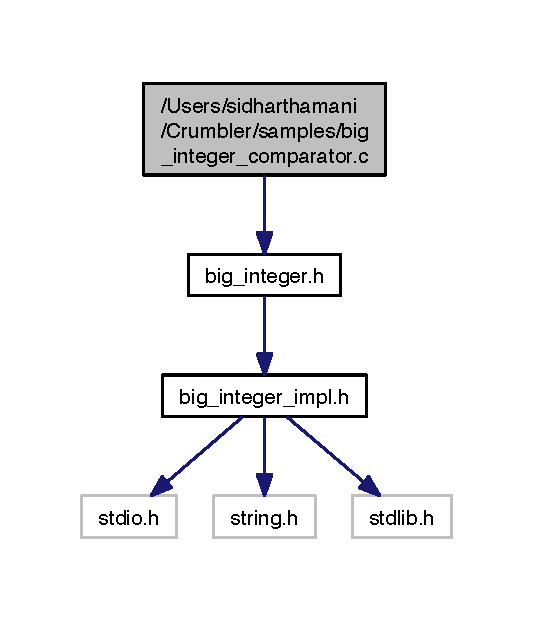
\includegraphics[width=256pt]{big__integer__comparator_8c__incl}
\end{center}
\end{figure}
\subsection*{Functions}
\begin{DoxyCompactItemize}
\item 
int \hyperlink{big__integer__comparator_8c_ae66f6b31b5ad750f1fe042a706a4e3d4}{main} ()
\end{DoxyCompactItemize}


\subsection{Detailed Description}
A sample implementation of \hyperlink{big__integer__impl_8h_structbig__integer}{big\-\_\-integer} comparison using crumbler library \par
 Author \-: Sidhartha Mani \par
 Contact \-: \href{mailto:sidharthamn@gmail.com}{\tt sidharthamn@gmail.\-com} \par
 Last updated on \-: 24 Dec 2012. 

Definition in file \hyperlink{}{big\-\_\-integer\-\_\-comparator.\-c}.



\subsection{Function Documentation}
\hypertarget{big__integer__comparator_8c_ae66f6b31b5ad750f1fe042a706a4e3d4}{\index{big\-\_\-integer\-\_\-comparator.\-c@{big\-\_\-integer\-\_\-comparator.\-c}!main@{main}}
\index{main@{main}!big_integer_comparator.c@{big\-\_\-integer\-\_\-comparator.\-c}}
\subsubsection[{main}]{\setlength{\rightskip}{0pt plus 5cm}int main (
\begin{DoxyParamCaption}
{}
\end{DoxyParamCaption}
)}}\label{big__integer__comparator_8c_ae66f6b31b5ad750f1fe042a706a4e3d4}


Definition at line 11 of file big\-\_\-integer\-\_\-comparator.\-c.


\begin{DoxyCode}
\{
    \textcolor{keywordtype}{char} integer1[2250];
    \textcolor{keywordtype}{char} integer2[2250];
    printf(\textcolor{stringliteral}{"Enter x\(\backslash\)n"});
    scanf(\textcolor{stringliteral}{"%s"},integer1);
    printf(\textcolor{stringliteral}{"Enter y\(\backslash\)n"});
    scanf(\textcolor{stringliteral}{"%s"},integer2);
    \textcolor{keyword}{struct }\hyperlink{struct_big___int}{Big\_Int} *x= \hyperlink{big__integer_8h_ae14e62d253605c66f8ff24d6ff75e5b9}{init\_Big\_Int\_from\_char}(
      integer1);
    \textcolor{keyword}{struct }\hyperlink{struct_big___int}{Big\_Int} *y = \hyperlink{big__integer_8h_ae14e62d253605c66f8ff24d6ff75e5b9}{init\_Big\_Int\_from\_char}(
      integer2);
    \textcolor{keywordtype}{int} compare = \hyperlink{big__integer_8h_a10fcd5cea7ae6f94061e05475c9ed397}{compare\_Big\_Ints}(x,y);
    \textcolor{keywordtype}{char} comparison\_message[50];
    \textcolor{keywordflow}{if}(compare == 0)
        sprintf(comparison\_message,\textcolor{stringliteral}{"the integers are equal"});
    \textcolor{keywordflow}{else} \textcolor{keywordflow}{if}(compare > 0)
        sprintf(comparison\_message,\textcolor{stringliteral}{"x is greater"});
    \textcolor{keywordflow}{else}
        sprintf(comparison\_message,\textcolor{stringliteral}{"y is greater"});    
    x = \hyperlink{big__integer_8h_a48953f2a94ebd2c4441734fca02005c0}{add\_Big\_Ints}(x,y,x);
    printf(\textcolor{stringliteral}{"%s\(\backslash\)nSUM: %s\(\backslash\)n"},comparison\_message,x->\hyperlink{struct_big___int_ac8d650b12656faee53d9ebd863e9fe8f}{get\_integer}(x));
    \hyperlink{big__integer_8c_a45174c2ae172f98bd7045eaaf7c51800}{destroy\_Big\_Int}(x);
    \hyperlink{big__integer_8c_a45174c2ae172f98bd7045eaaf7c51800}{destroy\_Big\_Int}(y);
    \textcolor{keywordflow}{return} 0;
\}\end{DoxyCode}

\hypertarget{simple__prefix__decoder_8c}{\section{/\-Users/sidharthamani/\-Crumbler/samples/simple\-\_\-prefix\-\_\-decoder.c File Reference}
\label{simple__prefix__decoder_8c}\index{/\-Users/sidharthamani/\-Crumbler/samples/simple\-\_\-prefix\-\_\-decoder.\-c@{/\-Users/sidharthamani/\-Crumbler/samples/simple\-\_\-prefix\-\_\-decoder.\-c}}
}


A sample implementation of simple prefix decoding using crumbler library \par
 Author \-: Sidhartha Mani \par
 Contact \-: \href{mailto:sidharthamn@gmail.com}{\tt sidharthamn@gmail.\-com} \par
 Last updated on \-: 24 Dec 2012.  


{\ttfamily \#include \char`\"{}simple\-\_\-prefix.\-h\char`\"{}}\\*
{\ttfamily \#include $<$stdio.\-h$>$}\\*
Include dependency graph for simple\-\_\-prefix\-\_\-decoder.\-c\-:\nopagebreak
\begin{figure}[H]
\begin{center}
\leavevmode
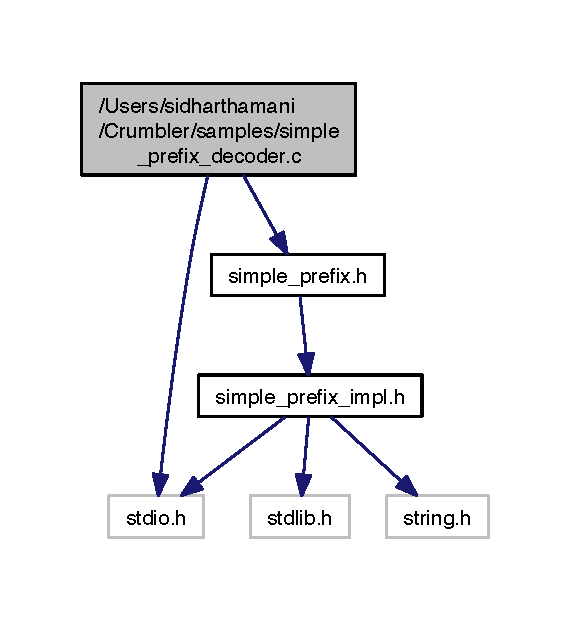
\includegraphics[width=274pt]{simple__prefix__decoder_8c__incl}
\end{center}
\end{figure}
\subsection*{Functions}
\begin{DoxyCompactItemize}
\item 
int \hyperlink{simple__prefix__decoder_8c_a3c04138a5bfe5d72780bb7e82a18e627}{main} (int argc, char $\ast$$\ast$argv)
\end{DoxyCompactItemize}


\subsection{Detailed Description}
A sample implementation of simple prefix decoding using crumbler library \par
 Author \-: Sidhartha Mani \par
 Contact \-: \href{mailto:sidharthamn@gmail.com}{\tt sidharthamn@gmail.\-com} \par
 Last updated on \-: 24 Dec 2012. 

Definition in file \hyperlink{}{simple\-\_\-prefix\-\_\-decoder.\-c}.



\subsection{Function Documentation}
\hypertarget{simple__prefix__decoder_8c_a3c04138a5bfe5d72780bb7e82a18e627}{\index{simple\-\_\-prefix\-\_\-decoder.\-c@{simple\-\_\-prefix\-\_\-decoder.\-c}!main@{main}}
\index{main@{main}!simple_prefix_decoder.c@{simple\-\_\-prefix\-\_\-decoder.\-c}}
\subsubsection[{main}]{\setlength{\rightskip}{0pt plus 5cm}int main (
\begin{DoxyParamCaption}
\item[{int}]{argc, }
\item[{char $\ast$$\ast$}]{argv}
\end{DoxyParamCaption}
)}}\label{simple__prefix__decoder_8c_a3c04138a5bfe5d72780bb7e82a18e627}


Definition at line 11 of file simple\-\_\-prefix\-\_\-decoder.\-c.


\begin{DoxyCode}
\{
    \textcolor{keywordflow}{if}(argc < 3)
    \{
        printf(\textcolor{stringliteral}{"Intructions : simple\_prefix input\_file output\_file\(\backslash\)n"});
        exit(0);
    \}
    \textcolor{keyword}{struct }\hyperlink{structsimple__prefix}{simple\_prefix} *decoder = \hyperlink{simple__prefix_8h_af2b9e30061b1c800008e5b55f93ab283}{init}();
    decoder->\hyperlink{structsimple__prefix_a58708e15f01f3be37e12d3194e953b41}{decode\_file}(argv[1],argv[2]);
    \textcolor{keywordflow}{return} 0;
    
    \textcolor{comment}{/* TO ENCODE , USE THIS AS AN EXAMPLE}
\textcolor{comment}{     struct simple\_prefix *encoder = init();}
\textcolor{comment}{     encoder->encode\_file("xyz","output");}
\textcolor{comment}{     return 0;}
\textcolor{comment}{     */}
\}\end{DoxyCode}

\hypertarget{simple__prefix__encoder_8c}{\section{/\-Users/sidharthamani/huffman\-\_\-coder/samples/simple\-\_\-prefix\-\_\-encoder.c File Reference}
\label{simple__prefix__encoder_8c}\index{/\-Users/sidharthamani/huffman\-\_\-coder/samples/simple\-\_\-prefix\-\_\-encoder.\-c@{/\-Users/sidharthamani/huffman\-\_\-coder/samples/simple\-\_\-prefix\-\_\-encoder.\-c}}
}


A sample implementation of simple prefix decoding using crumbler library \par
 Author \-: Sidhartha Mani \par
 Contact \-: \href{mailto:sidharthamn@gmail.com}{\tt sidharthamn@gmail.\-com} \par
 Last updated on \-: 24 Dec 2012.  


{\ttfamily \#include \char`\"{}simple\-\_\-prefix.\-h\char`\"{}}\\*
{\ttfamily \#include $<$stdio.\-h$>$}\\*
\subsection*{Functions}
\begin{DoxyCompactItemize}
\item 
int \hyperlink{simple__prefix__encoder_8c_a3c04138a5bfe5d72780bb7e82a18e627}{main} (int argc, char $\ast$$\ast$argv)
\end{DoxyCompactItemize}


\subsection{Detailed Description}
A sample implementation of simple prefix decoding using crumbler library \par
 Author \-: Sidhartha Mani \par
 Contact \-: \href{mailto:sidharthamn@gmail.com}{\tt sidharthamn@gmail.\-com} \par
 Last updated on \-: 24 Dec 2012. A sample implementation of simple prefix encoding using crumbler library \par
 Author \-: Sidhartha Mani \par
 Contact \-: \href{mailto:sidharthamn@gmail.com}{\tt sidharthamn@gmail.\-com} \par
 Last updated on \-: 24 Dec 2012.

Definition in file \hyperlink{}{simple\-\_\-prefix\-\_\-encoder.\-c}.



\subsection{Function Documentation}
\hypertarget{simple__prefix__encoder_8c_a3c04138a5bfe5d72780bb7e82a18e627}{\index{simple\-\_\-prefix\-\_\-encoder.\-c@{simple\-\_\-prefix\-\_\-encoder.\-c}!main@{main}}
\index{main@{main}!simple_prefix_encoder.c@{simple\-\_\-prefix\-\_\-encoder.\-c}}
\subsubsection[{main}]{\setlength{\rightskip}{0pt plus 5cm}int main (
\begin{DoxyParamCaption}
\item[{int}]{argc, }
\item[{char $\ast$$\ast$}]{argv}
\end{DoxyParamCaption}
)}}\label{simple__prefix__encoder_8c_a3c04138a5bfe5d72780bb7e82a18e627}


Definition at line 11 of file simple\-\_\-prefix\-\_\-encoder.\-c.


\begin{DoxyCode}
\{
    \textcolor{keywordflow}{if}(argc < 3)
    \{
        printf(\textcolor{stringliteral}{"Intructions : simple\_prefix input\_file output\_file\(\backslash\)n"});
        exit(0);
    \}
    \textcolor{keyword}{struct }\hyperlink{structsimple__prefix}{simple\_prefix} *encoder = \hyperlink{simple__prefix_8h_af2b9e30061b1c800008e5b55f93ab283}{init}();
    encoder->\hyperlink{structsimple__prefix_a73d0a239981b130553964b3839c20bdf}{encode\_file}(argv[1],argv[2]);
    \textcolor{keywordflow}{return} 0;
        
    \textcolor{comment}{/* TO DECODE , USE THIS AS AN EXAMPLE}
\textcolor{comment}{    struct simple\_prefix *decoder = init();}
\textcolor{comment}{    decoder->decode\_file("xyz","output");}
\textcolor{comment}{    return 0;}
\textcolor{comment}{    */}
\}
\end{DoxyCode}

\hypertarget{big__integer_8c}{\section{/\-Users/sidharthamani/huffman\-\_\-coder/src/big\-\_\-integer.c File Reference}
\label{big__integer_8c}\index{/\-Users/sidharthamani/huffman\-\_\-coder/src/big\-\_\-integer.\-c@{/\-Users/sidharthamani/huffman\-\_\-coder/src/big\-\_\-integer.\-c}}
}


The interface to the implementation of big integer logic This file contains functions required to interface with the big integer manipulation functions.\par
 Author \-: Sidhartha Mani\par
 Contact \-: \href{mailto:sidharthamn@gmail.com}{\tt sidharthamn@gmail.\-com} \par
 Last Updated \-: 24 Dec 2012 \par
  


{\ttfamily \#include \char`\"{}big\-\_\-integer.\-h\char`\"{}}\\*
\subsection*{Functions}
\begin{DoxyCompactItemize}
\item 
char $\ast$ \hyperlink{big__integer_8c_ab9e4a03f73b239e7b1b77623507f1325}{get\-\_\-integer\-\_\-as\-\_\-char} (\hyperlink{struct_big___int}{Big\-\_\-\-Int} $\ast$x)
\begin{DoxyCompactList}\small\item\em accessor to access the \hyperlink{big__integer__impl_8h_structbig__integer}{big\-\_\-integer} value \end{DoxyCompactList}\item 
int \hyperlink{big__integer_8c_a837651f373a264834cfb80be16d0ab32}{get\-\_\-sign\-\_\-as\-\_\-int} (\hyperlink{struct_big___int}{Big\-\_\-\-Int} $\ast$x)
\begin{DoxyCompactList}\small\item\em accessor to access the \hyperlink{big__integer__impl_8h_structbig__integer}{big\-\_\-integer} sign(+ve or -\/ve) \end{DoxyCompactList}\item 
void \hyperlink{big__integer_8c_a83fca4473e21f926f011b283b0cc7bc8}{set\-\_\-integer} (\hyperlink{struct_big___int}{Big\-\_\-\-Int} $\ast$x, char $\ast$y)
\begin{DoxyCompactList}\small\item\em sets the integer value of \hyperlink{struct_big___int}{Big\-\_\-\-Int} to the value pointed by param2 \end{DoxyCompactList}\item 
void \hyperlink{big__integer_8c_a1e8a8230d017886a82eb0a884f6fe12c}{set\-\_\-sign} (\hyperlink{struct_big___int}{Big\-\_\-\-Int} $\ast$x, int sign)
\begin{DoxyCompactList}\small\item\em sets the sign of \hyperlink{struct_big___int}{Big\-\_\-\-Int} to the value in param2 \end{DoxyCompactList}\item 
\hyperlink{struct_big___int}{Big\-\_\-\-Int} $\ast$ \hyperlink{big__integer_8c_ad2bdcff5870378868eebaebc64363bb4}{init\-\_\-\-Big\-\_\-\-Int} ()
\begin{DoxyCompactList}\small\item\em allocates memory for a new \hyperlink{struct_big___int}{Big\-\_\-\-Int} and returns a pointer to allocated memory \par
 {\bfseries  Precondition\-: } the pointer capturing the new memory should not have already been allocated memory \par
 {\bfseries  Postcondition\-: } the pointer is allocated memory \par
 \end{DoxyCompactList}\item 
\hyperlink{struct_big___int}{Big\-\_\-\-Int} $\ast$ \hyperlink{big__integer_8c_a09afd63acdaebc41e137d03aa2381a06}{init\-\_\-\-Big\-\_\-\-Int\-\_\-from\-\_\-char} (char $\ast$value)
\begin{DoxyCompactList}\small\item\em allocates memory for a new \hyperlink{struct_big___int}{Big\-\_\-\-Int}, initializes it to the value in value and returns a pointer to allocated memory. \par
 {\bfseries  Precondition\-: } the pointer capturing the new memory should not have already been allocated memory \par
 {\bfseries  Postcondition\-: } the pointer is initialized and allocated memory \par
 \end{DoxyCompactList}\item 
\hyperlink{struct_big___int}{Big\-\_\-\-Int} $\ast$ \hyperlink{big__integer_8c_a0c2885b6802e073ab77344b7323b4880}{init\-\_\-\-Big\-\_\-\-Int\-\_\-from\-\_\-long} (long long value)
\begin{DoxyCompactList}\small\item\em allocates memory for a new \hyperlink{struct_big___int}{Big\-\_\-\-Int}, initializes it to the value in value and returns a pointer to allocated memory. \par
 {\bfseries  Precondition\-: } the pointer capturing the new memory should not have already been allocated memory \par
 {\bfseries  Postcondition\-: } the pointer is initialized and allocated memory \par
 \end{DoxyCompactList}\item 
\hyperlink{struct_big___int}{Big\-\_\-\-Int} $\ast$ \hyperlink{big__integer_8c_a70280d3fbe2128f5bd1801dddcb781c1}{init\-\_\-\-Big\-\_\-\-Int\-\_\-from\-\_\-int} (int value)
\begin{DoxyCompactList}\small\item\em allocates memory for a new \hyperlink{struct_big___int}{Big\-\_\-\-Int}, initializes it to the value in value and returns a pointer to allocated memory. \par
 {\bfseries  Precondition\-: } the pointer capturing the new memory should not have already been allocated memory \par
 {\bfseries  Postcondition\-: } the pointer is initialized and allocated memory \par
 \end{DoxyCompactList}\item 
int \hyperlink{big__integer_8c_a10fcd5cea7ae6f94061e05475c9ed397}{compare\-\_\-\-Big\-\_\-\-Ints} (\hyperlink{struct_big___int}{Big\-\_\-\-Int} $\ast$operand1, \hyperlink{struct_big___int}{Big\-\_\-\-Int} $\ast$operand2)
\begin{DoxyCompactList}\small\item\em comapres two positive big integers only \par
 {\bfseries Precondition \-:} Both operand should have been initialized {\bfseries Postcondition \-:} The comparison result is provided \end{DoxyCompactList}\item 
void \hyperlink{big__integer_8c_a45174c2ae172f98bd7045eaaf7c51800}{destroy\-\_\-\-Big\-\_\-\-Int} (\hyperlink{struct_big___int}{Big\-\_\-\-Int} $\ast$obj)
\begin{DoxyCompactList}\small\item\em frees the allocated memory \par
 {\bfseries  Precondition\-: } the \hyperlink{struct_big___int}{Big\-\_\-\-Int} pointer which it is being freed should not have been freed already \par
 {\bfseries  Postcondition\-: }The \hyperlink{big__integer__impl_8h_structbig__integer}{big\-\_\-integer} structure is freed \end{DoxyCompactList}\item 
\hyperlink{struct_big___int}{Big\-\_\-\-Int} $\ast$ \hyperlink{big__integer_8c_a80b3b1955162bdbe4a92b73a576174a1}{add\-\_\-\-Big\-\_\-\-Ints} (\hyperlink{struct_big___int}{Big\-\_\-\-Int} $\ast$operand1, \hyperlink{struct_big___int}{Big\-\_\-\-Int} $\ast$operand2, \hyperlink{struct_big___int}{Big\-\_\-\-Int} $\ast$result)
\begin{DoxyCompactList}\small\item\em adds two positive integers only\par
 {\bfseries  Postcondition\-: }the \hyperlink{struct_big___int}{Big\-\_\-\-Int} object containing the sum is returned \end{DoxyCompactList}\end{DoxyCompactItemize}


\subsection{Detailed Description}
The interface to the implementation of big integer logic This file contains functions required to interface with the big integer manipulation functions.\par
 Author \-: Sidhartha Mani\par
 Contact \-: \href{mailto:sidharthamn@gmail.com}{\tt sidharthamn@gmail.\-com} \par
 Last Updated \-: 24 Dec 2012 \par
 

Definition in file \hyperlink{}{big\-\_\-integer.\-c}.



\subsection{Function Documentation}
\hypertarget{big__integer_8c_a80b3b1955162bdbe4a92b73a576174a1}{\index{big\-\_\-integer.\-c@{big\-\_\-integer.\-c}!add\-\_\-\-Big\-\_\-\-Ints@{add\-\_\-\-Big\-\_\-\-Ints}}
\index{add\-\_\-\-Big\-\_\-\-Ints@{add\-\_\-\-Big\-\_\-\-Ints}!big_integer.c@{big\-\_\-integer.\-c}}
\subsubsection[{add\-\_\-\-Big\-\_\-\-Ints}]{\setlength{\rightskip}{0pt plus 5cm}{\bf Big\-\_\-\-Int}$\ast$ add\-\_\-\-Big\-\_\-\-Ints (
\begin{DoxyParamCaption}
\item[{{\bf Big\-\_\-\-Int} $\ast$}]{operand1, }
\item[{{\bf Big\-\_\-\-Int} $\ast$}]{operand2, }
\item[{{\bf Big\-\_\-\-Int} $\ast$}]{result}
\end{DoxyParamCaption}
)}}\label{big__integer_8c_a80b3b1955162bdbe4a92b73a576174a1}


adds two positive integers only\par
 {\bfseries  Postcondition\-: }the \hyperlink{struct_big___int}{Big\-\_\-\-Int} object containing the sum is returned 


\begin{DoxyParams}{Parameters}
{\em operand1} & the first \hyperlink{struct_big___int}{Big\-\_\-\-Int} operand for addition \\
\hline
{\em operand2} & the second \hyperlink{struct_big___int}{Big\-\_\-\-Int} operand for addition \\
\hline
{\em result} & the \hyperlink{struct_big___int}{Big\-\_\-\-Int} structure in which the result should be stored, its ok if it was previously initialized or not \\
\hline
\end{DoxyParams}
\begin{DoxyReturn}{Returns}
a pointer to the \hyperlink{struct_big___int}{Big\-\_\-\-Int} holding the sum 
\end{DoxyReturn}


Definition at line 172 of file big\-\_\-integer.\-c.


\begin{DoxyCode}
\{
    \textcolor{keyword}{struct }\hyperlink{struct_big___int}{Big\_Int} *temp = \hyperlink{big__integer_8h_a20af4609c2f9d837a45de3b064f3db2c}{init\_Big\_Int}();
    temp->\hyperlink{struct_big___int_af78495b20eeda6242727ea99032693c2}{integer} = \hyperlink{big__integer__impl_8h_acaa9b81fceecc01e260e7011fda3d628}{add\_big\_integers}(operand1->\hyperlink{struct_big___int_af78495b20eeda6242727ea99032693c2}{integer}
      ,operand2->\hyperlink{struct_big___int_af78495b20eeda6242727ea99032693c2}{integer},temp->\hyperlink{struct_big___int_af78495b20eeda6242727ea99032693c2}{integer});
    \hyperlink{big__integer_8c_a45174c2ae172f98bd7045eaaf7c51800}{destroy\_Big\_Int}(result);
    result = temp;
    \textcolor{keywordflow}{return} result;
\}
\end{DoxyCode}
\hypertarget{big__integer_8c_a10fcd5cea7ae6f94061e05475c9ed397}{\index{big\-\_\-integer.\-c@{big\-\_\-integer.\-c}!compare\-\_\-\-Big\-\_\-\-Ints@{compare\-\_\-\-Big\-\_\-\-Ints}}
\index{compare\-\_\-\-Big\-\_\-\-Ints@{compare\-\_\-\-Big\-\_\-\-Ints}!big_integer.c@{big\-\_\-integer.\-c}}
\subsubsection[{compare\-\_\-\-Big\-\_\-\-Ints}]{\setlength{\rightskip}{0pt plus 5cm}int compare\-\_\-\-Big\-\_\-\-Ints (
\begin{DoxyParamCaption}
\item[{{\bf Big\-\_\-\-Int} $\ast$}]{operand1, }
\item[{{\bf Big\-\_\-\-Int} $\ast$}]{operand2}
\end{DoxyParamCaption}
)}}\label{big__integer_8c_a10fcd5cea7ae6f94061e05475c9ed397}


comapres two positive big integers only \par
 {\bfseries Precondition \-:} Both operand should have been initialized {\bfseries Postcondition \-:} The comparison result is provided 


\begin{DoxyParams}{Parameters}
{\em operand1} & the operand against which the other operand will be compared \\
\hline
{\em operand2} & the operand which will be compared against operand1 \\
\hline
\end{DoxyParams}
\begin{DoxyReturn}{Returns}
\par
 Returns 0 \-: if both numbers are equal \par
 Returns $>$ 0 \-: if first value is larger \par
 Returns $<$ 0 \-: if first value is smaller 
\end{DoxyReturn}


Definition at line 146 of file big\-\_\-integer.\-c.


\begin{DoxyCode}
\{
    \textcolor{keywordflow}{return} \hyperlink{big__integer__impl_8h_a12e0894b8887892194604e1217fe2afd}{compare\_big\_integers}(operand1->\hyperlink{struct_big___int_af78495b20eeda6242727ea99032693c2}{integer},
      operand2->\hyperlink{struct_big___int_af78495b20eeda6242727ea99032693c2}{integer});
\}
\end{DoxyCode}
\hypertarget{big__integer_8c_a45174c2ae172f98bd7045eaaf7c51800}{\index{big\-\_\-integer.\-c@{big\-\_\-integer.\-c}!destroy\-\_\-\-Big\-\_\-\-Int@{destroy\-\_\-\-Big\-\_\-\-Int}}
\index{destroy\-\_\-\-Big\-\_\-\-Int@{destroy\-\_\-\-Big\-\_\-\-Int}!big_integer.c@{big\-\_\-integer.\-c}}
\subsubsection[{destroy\-\_\-\-Big\-\_\-\-Int}]{\setlength{\rightskip}{0pt plus 5cm}void destroy\-\_\-\-Big\-\_\-\-Int (
\begin{DoxyParamCaption}
\item[{{\bf Big\-\_\-\-Int} $\ast$}]{obj}
\end{DoxyParamCaption}
)}}\label{big__integer_8c_a45174c2ae172f98bd7045eaaf7c51800}


frees the allocated memory \par
 {\bfseries  Precondition\-: } the \hyperlink{struct_big___int}{Big\-\_\-\-Int} pointer which it is being freed should not have been freed already \par
 {\bfseries  Postcondition\-: }The \hyperlink{big__integer__impl_8h_structbig__integer}{big\-\_\-integer} structure is freed 


\begin{DoxyParams}{Parameters}
{\em operand1} & the pointer to the structure which should be freed \\
\hline
\end{DoxyParams}
\begin{DoxyReturn}{Returns}
Nothing 
\end{DoxyReturn}


Definition at line 158 of file big\-\_\-integer.\-c.


\begin{DoxyCode}
\{
    \hyperlink{big__integer__impl_8h_aba3732c4704a6c73493683133fcd9cae}{destroy\_big\_integer}(obj->\hyperlink{struct_big___int_af78495b20eeda6242727ea99032693c2}{integer});
    free(obj);
\}
\end{DoxyCode}
\hypertarget{big__integer_8c_ab9e4a03f73b239e7b1b77623507f1325}{\index{big\-\_\-integer.\-c@{big\-\_\-integer.\-c}!get\-\_\-integer\-\_\-as\-\_\-char@{get\-\_\-integer\-\_\-as\-\_\-char}}
\index{get\-\_\-integer\-\_\-as\-\_\-char@{get\-\_\-integer\-\_\-as\-\_\-char}!big_integer.c@{big\-\_\-integer.\-c}}
\subsubsection[{get\-\_\-integer\-\_\-as\-\_\-char}]{\setlength{\rightskip}{0pt plus 5cm}char $\ast$ get\-\_\-integer\-\_\-as\-\_\-char (
\begin{DoxyParamCaption}
\item[{{\bf Big\-\_\-\-Int} $\ast$}]{x}
\end{DoxyParamCaption}
)}}\label{big__integer_8c_ab9e4a03f73b239e7b1b77623507f1325}


accessor to access the \hyperlink{big__integer__impl_8h_structbig__integer}{big\-\_\-integer} value 


\begin{DoxyParams}{Parameters}
{\em a} & pointer to self \\
\hline
\end{DoxyParams}
\begin{DoxyReturn}{Returns}
a char array that contains the \hyperlink{big__integer__impl_8h_structbig__integer}{big\-\_\-integer} value as a string 
\end{DoxyReturn}


Definition at line 18 of file big\-\_\-integer.\-c.


\begin{DoxyCode}
\{
    \textcolor{keywordflow}{return} x->\hyperlink{struct_big___int_af78495b20eeda6242727ea99032693c2}{integer}->\hyperlink{big__integer__impl_8h_a4e9aec275e566b978a3ccb4e043d8c61}{value};
\}
\end{DoxyCode}
\hypertarget{big__integer_8c_a837651f373a264834cfb80be16d0ab32}{\index{big\-\_\-integer.\-c@{big\-\_\-integer.\-c}!get\-\_\-sign\-\_\-as\-\_\-int@{get\-\_\-sign\-\_\-as\-\_\-int}}
\index{get\-\_\-sign\-\_\-as\-\_\-int@{get\-\_\-sign\-\_\-as\-\_\-int}!big_integer.c@{big\-\_\-integer.\-c}}
\subsubsection[{get\-\_\-sign\-\_\-as\-\_\-int}]{\setlength{\rightskip}{0pt plus 5cm}int get\-\_\-sign\-\_\-as\-\_\-int (
\begin{DoxyParamCaption}
\item[{{\bf Big\-\_\-\-Int} $\ast$}]{x}
\end{DoxyParamCaption}
)}}\label{big__integer_8c_a837651f373a264834cfb80be16d0ab32}


accessor to access the \hyperlink{big__integer__impl_8h_structbig__integer}{big\-\_\-integer} sign(+ve or -\/ve) 


\begin{DoxyParams}{Parameters}
{\em a} & pointer to self \\
\hline
\end{DoxyParams}
\begin{DoxyReturn}{Returns}
\par
 Returns $>$=0, if positive \par
 Returns $<$ 0, if negative 
\end{DoxyReturn}


Definition at line 30 of file big\-\_\-integer.\-c.


\begin{DoxyCode}
\{
    \textcolor{keywordflow}{return} x->\hyperlink{struct_big___int_af78495b20eeda6242727ea99032693c2}{integer}->\hyperlink{big__integer__impl_8h_abbeb8ae63622a7fef0b5a56bb91a1682}{sign};
\}
\end{DoxyCode}
\hypertarget{big__integer_8c_ad2bdcff5870378868eebaebc64363bb4}{\index{big\-\_\-integer.\-c@{big\-\_\-integer.\-c}!init\-\_\-\-Big\-\_\-\-Int@{init\-\_\-\-Big\-\_\-\-Int}}
\index{init\-\_\-\-Big\-\_\-\-Int@{init\-\_\-\-Big\-\_\-\-Int}!big_integer.c@{big\-\_\-integer.\-c}}
\subsubsection[{init\-\_\-\-Big\-\_\-\-Int}]{\setlength{\rightskip}{0pt plus 5cm}{\bf Big\-\_\-\-Int}$\ast$ init\-\_\-\-Big\-\_\-\-Int (
\begin{DoxyParamCaption}
{}
\end{DoxyParamCaption}
)}}\label{big__integer_8c_ad2bdcff5870378868eebaebc64363bb4}


allocates memory for a new \hyperlink{struct_big___int}{Big\-\_\-\-Int} and returns a pointer to allocated memory \par
 {\bfseries  Precondition\-: } the pointer capturing the new memory should not have already been allocated memory \par
 {\bfseries  Postcondition\-: } the pointer is allocated memory \par
 

\begin{DoxyReturn}{Returns}
a pointer to the newly allocated memory to hold a \hyperlink{struct_big___int}{Big\-\_\-\-Int} variable 
\end{DoxyReturn}


Definition at line 67 of file big\-\_\-integer.\-c.


\begin{DoxyCode}
\{
    \textcolor{keyword}{struct }\hyperlink{struct_big___int}{Big\_Int} *temp = (\textcolor{keyword}{struct }\hyperlink{struct_big___int}{Big\_Int}*)malloc(\textcolor{keyword}{sizeof}(\textcolor{keyword}{struct} 
      \hyperlink{struct_big___int}{Big\_Int}));
    temp->\hyperlink{struct_big___int_af78495b20eeda6242727ea99032693c2}{integer} = \hyperlink{big__integer__impl_8h_ad427e9cea709aee7a823b0136216fbfc}{init\_big\_integer}();
    temp->\hyperlink{struct_big___int_ac8d650b12656faee53d9ebd863e9fe8f}{get\_integer} = \hyperlink{big__integer_8c_ab9e4a03f73b239e7b1b77623507f1325}{get\_integer\_as\_char};
    temp->\hyperlink{struct_big___int_ae06ba678ba07ecdac264605bc8576da2}{get\_sign} = \hyperlink{big__integer_8c_a837651f373a264834cfb80be16d0ab32}{get\_sign\_as\_int};
    temp->\hyperlink{struct_big___int_a34a65fb8d8cc2acf5a14a18c420ee774}{set\_integer} = \hyperlink{big__integer_8c_a83fca4473e21f926f011b283b0cc7bc8}{set\_integer};
    temp->\hyperlink{struct_big___int_a70cf790b3af136aad25fa028cde3e801}{set\_sign} = \hyperlink{big__integer_8c_a1e8a8230d017886a82eb0a884f6fe12c}{set\_sign};
    \textcolor{keywordflow}{return} temp;
\}
\end{DoxyCode}
\hypertarget{big__integer_8c_a09afd63acdaebc41e137d03aa2381a06}{\index{big\-\_\-integer.\-c@{big\-\_\-integer.\-c}!init\-\_\-\-Big\-\_\-\-Int\-\_\-from\-\_\-char@{init\-\_\-\-Big\-\_\-\-Int\-\_\-from\-\_\-char}}
\index{init\-\_\-\-Big\-\_\-\-Int\-\_\-from\-\_\-char@{init\-\_\-\-Big\-\_\-\-Int\-\_\-from\-\_\-char}!big_integer.c@{big\-\_\-integer.\-c}}
\subsubsection[{init\-\_\-\-Big\-\_\-\-Int\-\_\-from\-\_\-char}]{\setlength{\rightskip}{0pt plus 5cm}{\bf Big\-\_\-\-Int}$\ast$ init\-\_\-\-Big\-\_\-\-Int\-\_\-from\-\_\-char (
\begin{DoxyParamCaption}
\item[{char $\ast$}]{value}
\end{DoxyParamCaption}
)}}\label{big__integer_8c_a09afd63acdaebc41e137d03aa2381a06}


allocates memory for a new \hyperlink{struct_big___int}{Big\-\_\-\-Int}, initializes it to the value in value and returns a pointer to allocated memory. \par
 {\bfseries  Precondition\-: } the pointer capturing the new memory should not have already been allocated memory \par
 {\bfseries  Postcondition\-: } the pointer is initialized and allocated memory \par
 


\begin{DoxyParams}{Parameters}
{\em value} & the value that will be copied into the new \hyperlink{big__integer__impl_8h_structbig__integer}{big\-\_\-integer} \\
\hline
\end{DoxyParams}
\begin{DoxyReturn}{Returns}
a pointer to the newly allocated memory to hold a \hyperlink{struct_big___int}{Big\-\_\-\-Int} variable containing the value in value 
\end{DoxyReturn}


Definition at line 86 of file big\-\_\-integer.\-c.


\begin{DoxyCode}
\{
    \textcolor{keyword}{struct }\hyperlink{struct_big___int}{Big\_Int} *temp = (\textcolor{keyword}{struct }\hyperlink{struct_big___int}{Big\_Int}*)malloc(\textcolor{keyword}{sizeof}(\textcolor{keyword}{struct} 
      \hyperlink{struct_big___int}{Big\_Int}));
    temp->\hyperlink{struct_big___int_af78495b20eeda6242727ea99032693c2}{integer} =\hyperlink{big__integer__impl_8h_a78fe148b385a4ccb53b8b6c9cac949cb}{init\_big\_integer\_from\_char}(
      value);
    temp->\hyperlink{struct_big___int_ac8d650b12656faee53d9ebd863e9fe8f}{get\_integer} = \hyperlink{big__integer_8c_ab9e4a03f73b239e7b1b77623507f1325}{get\_integer\_as\_char};
    temp->\hyperlink{struct_big___int_ae06ba678ba07ecdac264605bc8576da2}{get\_sign} = \hyperlink{big__integer_8c_a837651f373a264834cfb80be16d0ab32}{get\_sign\_as\_int};
    temp->\hyperlink{struct_big___int_a34a65fb8d8cc2acf5a14a18c420ee774}{set\_integer} = \hyperlink{big__integer_8c_a83fca4473e21f926f011b283b0cc7bc8}{set\_integer};
    temp->\hyperlink{struct_big___int_a70cf790b3af136aad25fa028cde3e801}{set\_sign} = \hyperlink{big__integer_8c_a1e8a8230d017886a82eb0a884f6fe12c}{set\_sign};
    \textcolor{keywordflow}{return} temp;
\}
\end{DoxyCode}
\hypertarget{big__integer_8c_a70280d3fbe2128f5bd1801dddcb781c1}{\index{big\-\_\-integer.\-c@{big\-\_\-integer.\-c}!init\-\_\-\-Big\-\_\-\-Int\-\_\-from\-\_\-int@{init\-\_\-\-Big\-\_\-\-Int\-\_\-from\-\_\-int}}
\index{init\-\_\-\-Big\-\_\-\-Int\-\_\-from\-\_\-int@{init\-\_\-\-Big\-\_\-\-Int\-\_\-from\-\_\-int}!big_integer.c@{big\-\_\-integer.\-c}}
\subsubsection[{init\-\_\-\-Big\-\_\-\-Int\-\_\-from\-\_\-int}]{\setlength{\rightskip}{0pt plus 5cm}{\bf Big\-\_\-\-Int}$\ast$ init\-\_\-\-Big\-\_\-\-Int\-\_\-from\-\_\-int (
\begin{DoxyParamCaption}
\item[{int}]{value}
\end{DoxyParamCaption}
)}}\label{big__integer_8c_a70280d3fbe2128f5bd1801dddcb781c1}


allocates memory for a new \hyperlink{struct_big___int}{Big\-\_\-\-Int}, initializes it to the value in value and returns a pointer to allocated memory. \par
 {\bfseries  Precondition\-: } the pointer capturing the new memory should not have already been allocated memory \par
 {\bfseries  Postcondition\-: } the pointer is initialized and allocated memory \par
 


\begin{DoxyParams}{Parameters}
{\em value} & the value that will be copied into the new \hyperlink{big__integer__impl_8h_structbig__integer}{big\-\_\-integer} \\
\hline
\end{DoxyParams}
\begin{DoxyReturn}{Returns}
a pointer to the newly allocated memory to hold a \hyperlink{struct_big___int}{Big\-\_\-\-Int} variable containing the value in value 
\end{DoxyReturn}


Definition at line 124 of file big\-\_\-integer.\-c.


\begin{DoxyCode}
\{
    \textcolor{keyword}{struct }\hyperlink{struct_big___int}{Big\_Int} *temp = (\textcolor{keyword}{struct }\hyperlink{struct_big___int}{Big\_Int}*)malloc(\textcolor{keyword}{sizeof}(\textcolor{keyword}{struct} 
      \hyperlink{struct_big___int}{Big\_Int}));
    temp->\hyperlink{struct_big___int_af78495b20eeda6242727ea99032693c2}{integer} = \hyperlink{big__integer__impl_8h_aba2b222c87a6ad23da34a0c8000e2506}{init\_big\_integer\_from\_int}(
      value);
    temp->\hyperlink{struct_big___int_ac8d650b12656faee53d9ebd863e9fe8f}{get\_integer} = \hyperlink{big__integer_8c_ab9e4a03f73b239e7b1b77623507f1325}{get\_integer\_as\_char};
    temp->\hyperlink{struct_big___int_ae06ba678ba07ecdac264605bc8576da2}{get\_sign} = \hyperlink{big__integer_8c_a837651f373a264834cfb80be16d0ab32}{get\_sign\_as\_int};
    temp->\hyperlink{struct_big___int_a34a65fb8d8cc2acf5a14a18c420ee774}{set\_integer} = \hyperlink{big__integer_8c_a83fca4473e21f926f011b283b0cc7bc8}{set\_integer};
    temp->\hyperlink{struct_big___int_a70cf790b3af136aad25fa028cde3e801}{set\_sign} = \hyperlink{big__integer_8c_a1e8a8230d017886a82eb0a884f6fe12c}{set\_sign};
    \textcolor{keywordflow}{return} temp;
\}
\end{DoxyCode}
\hypertarget{big__integer_8c_a0c2885b6802e073ab77344b7323b4880}{\index{big\-\_\-integer.\-c@{big\-\_\-integer.\-c}!init\-\_\-\-Big\-\_\-\-Int\-\_\-from\-\_\-long@{init\-\_\-\-Big\-\_\-\-Int\-\_\-from\-\_\-long}}
\index{init\-\_\-\-Big\-\_\-\-Int\-\_\-from\-\_\-long@{init\-\_\-\-Big\-\_\-\-Int\-\_\-from\-\_\-long}!big_integer.c@{big\-\_\-integer.\-c}}
\subsubsection[{init\-\_\-\-Big\-\_\-\-Int\-\_\-from\-\_\-long}]{\setlength{\rightskip}{0pt plus 5cm}{\bf Big\-\_\-\-Int}$\ast$ init\-\_\-\-Big\-\_\-\-Int\-\_\-from\-\_\-long (
\begin{DoxyParamCaption}
\item[{long long}]{value}
\end{DoxyParamCaption}
)}}\label{big__integer_8c_a0c2885b6802e073ab77344b7323b4880}


allocates memory for a new \hyperlink{struct_big___int}{Big\-\_\-\-Int}, initializes it to the value in value and returns a pointer to allocated memory. \par
 {\bfseries  Precondition\-: } the pointer capturing the new memory should not have already been allocated memory \par
 {\bfseries  Postcondition\-: } the pointer is initialized and allocated memory \par
 


\begin{DoxyParams}{Parameters}
{\em value} & the value that will be copied into the new \hyperlink{big__integer__impl_8h_structbig__integer}{big\-\_\-integer} \\
\hline
\end{DoxyParams}
\begin{DoxyReturn}{Returns}
a pointer to the newly allocated memory to hold a \hyperlink{struct_big___int}{Big\-\_\-\-Int} variable containing the value in value 
\end{DoxyReturn}


Definition at line 105 of file big\-\_\-integer.\-c.


\begin{DoxyCode}
\{
    \textcolor{keyword}{struct }\hyperlink{struct_big___int}{Big\_Int} *temp = (\textcolor{keyword}{struct }\hyperlink{struct_big___int}{Big\_Int}*)malloc(\textcolor{keyword}{sizeof}(\textcolor{keyword}{struct} 
      \hyperlink{struct_big___int}{Big\_Int}));
    temp->\hyperlink{struct_big___int_af78495b20eeda6242727ea99032693c2}{integer} = \hyperlink{big__integer__impl_8h_a1329d3ba57def63a30fa2244a547eb29}{init\_big\_integer\_from\_long}
      (value);
    temp->\hyperlink{struct_big___int_ac8d650b12656faee53d9ebd863e9fe8f}{get\_integer} = \hyperlink{big__integer_8c_ab9e4a03f73b239e7b1b77623507f1325}{get\_integer\_as\_char};
    temp->\hyperlink{struct_big___int_ae06ba678ba07ecdac264605bc8576da2}{get\_sign} = \hyperlink{big__integer_8c_a837651f373a264834cfb80be16d0ab32}{get\_sign\_as\_int};
    temp->\hyperlink{struct_big___int_a34a65fb8d8cc2acf5a14a18c420ee774}{set\_integer} = \hyperlink{big__integer_8c_a83fca4473e21f926f011b283b0cc7bc8}{set\_integer};
    temp->\hyperlink{struct_big___int_a70cf790b3af136aad25fa028cde3e801}{set\_sign} = \hyperlink{big__integer_8c_a1e8a8230d017886a82eb0a884f6fe12c}{set\_sign};
    \textcolor{keywordflow}{return} temp;
\}
\end{DoxyCode}
\hypertarget{big__integer_8c_a83fca4473e21f926f011b283b0cc7bc8}{\index{big\-\_\-integer.\-c@{big\-\_\-integer.\-c}!set\-\_\-integer@{set\-\_\-integer}}
\index{set\-\_\-integer@{set\-\_\-integer}!big_integer.c@{big\-\_\-integer.\-c}}
\subsubsection[{set\-\_\-integer}]{\setlength{\rightskip}{0pt plus 5cm}void set\-\_\-integer (
\begin{DoxyParamCaption}
\item[{{\bf Big\-\_\-\-Int} $\ast$}]{x, }
\item[{char $\ast$}]{y}
\end{DoxyParamCaption}
)}}\label{big__integer_8c_a83fca4473e21f926f011b283b0cc7bc8}


sets the integer value of \hyperlink{struct_big___int}{Big\-\_\-\-Int} to the value pointed by param2 


\begin{DoxyParams}{Parameters}
{\em x} & a pointer to self \\
\hline
{\em y} & a pointer to the new value \\
\hline
\end{DoxyParams}
\begin{DoxyReturn}{Returns}
Nothing 
\end{DoxyReturn}


Definition at line 41 of file big\-\_\-integer.\-c.


\begin{DoxyCode}
\{
    free(x->\hyperlink{struct_big___int_af78495b20eeda6242727ea99032693c2}{integer}->\hyperlink{big__integer__impl_8h_a4e9aec275e566b978a3ccb4e043d8c61}{value});
    x->\hyperlink{struct_big___int_af78495b20eeda6242727ea99032693c2}{integer}->\hyperlink{big__integer__impl_8h_a4e9aec275e566b978a3ccb4e043d8c61}{value} = (\textcolor{keywordtype}{char}*)malloc(strlen(y));
    memcpy(x->\hyperlink{struct_big___int_af78495b20eeda6242727ea99032693c2}{integer}->\hyperlink{big__integer__impl_8h_a4e9aec275e566b978a3ccb4e043d8c61}{value},y,strlen(y));
\}
\end{DoxyCode}
\hypertarget{big__integer_8c_a1e8a8230d017886a82eb0a884f6fe12c}{\index{big\-\_\-integer.\-c@{big\-\_\-integer.\-c}!set\-\_\-sign@{set\-\_\-sign}}
\index{set\-\_\-sign@{set\-\_\-sign}!big_integer.c@{big\-\_\-integer.\-c}}
\subsubsection[{set\-\_\-sign}]{\setlength{\rightskip}{0pt plus 5cm}void set\-\_\-sign (
\begin{DoxyParamCaption}
\item[{{\bf Big\-\_\-\-Int} $\ast$}]{x, }
\item[{int}]{sign}
\end{DoxyParamCaption}
)}}\label{big__integer_8c_a1e8a8230d017886a82eb0a884f6fe12c}


sets the sign of \hyperlink{struct_big___int}{Big\-\_\-\-Int} to the value in param2 


\begin{DoxyParams}{Parameters}
{\em x} & a pointer to self \\
\hline
{\em sign} & the sign of the \hyperlink{struct_big___int}{Big\-\_\-\-Int} \par
 sign $>$=0, if positive \par
 sign $<$ 0, if negative \\
\hline
\end{DoxyParams}
\begin{DoxyReturn}{Returns}
Nothing 
\end{DoxyReturn}


Definition at line 56 of file big\-\_\-integer.\-c.


\begin{DoxyCode}
\{
    x->\hyperlink{struct_big___int_af78495b20eeda6242727ea99032693c2}{integer}->\hyperlink{big__integer__impl_8h_abbeb8ae63622a7fef0b5a56bb91a1682}{sign} = sign;
\}
\end{DoxyCode}

\hypertarget{big__integer__impl_8c}{\section{/\-Users/sidharthamani/huffman\-\_\-coder/src/big\-\_\-integer\-\_\-impl.c File Reference}
\label{big__integer__impl_8c}\index{/\-Users/sidharthamani/huffman\-\_\-coder/src/big\-\_\-integer\-\_\-impl.\-c@{/\-Users/sidharthamani/huffman\-\_\-coder/src/big\-\_\-integer\-\_\-impl.\-c}}
}
{\ttfamily \#include \char`\"{}big\-\_\-integer\-\_\-impl.\-h\char`\"{}}\\*
Include dependency graph for big\-\_\-integer\-\_\-impl.\-c\-:
\subsection*{Functions}
\begin{DoxyCompactItemize}
\item 
char $\ast$ \hyperlink{big__integer__impl_8c_a8242235fbc1f6d24b8de1dda59b5c5cf}{reverse\-\_\-string} (char $\ast$string)
\item 
char $\ast$ \hyperlink{big__integer__impl_8c_a8906be19bb42c9a4ac1cb54387ee01d0}{long\-\_\-long\-\_\-to\-\_\-char} (long long long\-\_\-long\-\_\-value)
\item 
\hyperlink{structbig__integer}{big\-\_\-integer} $\ast$ \hyperlink{big__integer__impl_8c_a12a72eb0245b2fbd9cce5dacaf877a72}{init\-\_\-big\-\_\-integer} ()
\item 
\hyperlink{structbig__integer}{big\-\_\-integer} $\ast$ \hyperlink{big__integer__impl_8c_a2ea84ff52859d3887e65b120068c0158}{init\-\_\-big\-\_\-integer\-\_\-from\-\_\-long} (long long long\-\_\-long\-\_\-value)
\item 
\hyperlink{structbig__integer}{big\-\_\-integer} $\ast$ \hyperlink{big__integer__impl_8c_a4c0bcb12462f0ee91ab4e2a50648959d}{init\-\_\-big\-\_\-integer\-\_\-from\-\_\-int} (int int\-\_\-value)
\item 
\hyperlink{structbig__integer}{big\-\_\-integer} $\ast$ \hyperlink{big__integer__impl_8c_aa901ea9fc65455e5956685f79de483f5}{init\-\_\-big\-\_\-integer\-\_\-from\-\_\-char} (char $\ast$value)
\item 
int \hyperlink{big__integer__impl_8c_a12e0894b8887892194604e1217fe2afd}{compare\-\_\-big\-\_\-integers} (struct \hyperlink{structbig__integer}{big\-\_\-integer} $\ast$operand1, struct \hyperlink{structbig__integer}{big\-\_\-integer} $\ast$operand2)
\item 
void \hyperlink{big__integer__impl_8c_aba3732c4704a6c73493683133fcd9cae}{destroy\-\_\-big\-\_\-integer} (\hyperlink{structbig__integer}{big\-\_\-integer} $\ast$obj)
\item 
\hyperlink{structbig__integer}{big\-\_\-integer} $\ast$ \hyperlink{big__integer__impl_8c_a166ce246dbb5f170130a647c7b3fabe7}{add\-\_\-big\-\_\-integers} (struct \hyperlink{structbig__integer}{big\-\_\-integer} $\ast$operand1, struct \hyperlink{structbig__integer}{big\-\_\-integer} $\ast$operand2, struct \hyperlink{structbig__integer}{big\-\_\-integer} $\ast$result)
\end{DoxyCompactItemize}


\subsection{Function Documentation}
\hypertarget{big__integer__impl_8c_a166ce246dbb5f170130a647c7b3fabe7}{\index{big\-\_\-integer\-\_\-impl.\-c@{big\-\_\-integer\-\_\-impl.\-c}!add\-\_\-big\-\_\-integers@{add\-\_\-big\-\_\-integers}}
\index{add\-\_\-big\-\_\-integers@{add\-\_\-big\-\_\-integers}!big_integer_impl.c@{big\-\_\-integer\-\_\-impl.\-c}}
\subsubsection[{add\-\_\-big\-\_\-integers}]{\setlength{\rightskip}{0pt plus 5cm}{\bf big\-\_\-integer}$\ast$ add\-\_\-big\-\_\-integers (
\begin{DoxyParamCaption}
\item[{struct {\bf big\-\_\-integer} $\ast$}]{operand1, }
\item[{struct {\bf big\-\_\-integer} $\ast$}]{operand2, }
\item[{struct {\bf big\-\_\-integer} $\ast$}]{result}
\end{DoxyParamCaption}
)}}\label{big__integer__impl_8c_a166ce246dbb5f170130a647c7b3fabe7}

\begin{DoxyCode}
\{
    \textcolor{keywordtype}{int} larger=(\hyperlink{big__integer__impl_8h_a12e0894b8887892194604e1217fe2afd}{compare\_big\_integers}(operand1,operand2)>=0)
      ?1:2;
    \textcolor{keywordtype}{char} new\_value[larger==1?strlen(operand1->\hyperlink{structbig__integer_a4e9aec275e566b978a3ccb4e043d8c61}{value})+2:strlen(operand2->
      \hyperlink{structbig__integer_a4e9aec275e566b978a3ccb4e043d8c61}{value})+2];
    new\_value[0] = \textcolor{charliteral}{'0'};
    new\_value[\textcolor{keyword}{sizeof}(new\_value) - 1] = \textcolor{charliteral}{'\(\backslash\)0'};
    \textcolor{keyword}{struct }\hyperlink{structbig__integer}{big\_integer} *larger\_integer = (larger==1?operand1:
      operand2);  
    \textcolor{keyword}{struct }\hyperlink{structbig__integer}{big\_integer} *shorter\_integer = (larger==2?operand1:
      operand2);
    \textcolor{keywordtype}{int} i = strlen(larger\_integer->\hyperlink{structbig__integer_a4e9aec275e566b978a3ccb4e043d8c61}{value});
    \textcolor{keywordtype}{int} j = strlen(shorter\_integer->\hyperlink{structbig__integer_a4e9aec275e566b978a3ccb4e043d8c61}{value}) - 1;
    \textcolor{keywordtype}{int} k = strlen(larger\_integer->\hyperlink{structbig__integer_a4e9aec275e566b978a3ccb4e043d8c61}{value});
    \textcolor{keywordtype}{int} sum;
    \textcolor{keywordtype}{int} carry = 0;
    \textcolor{keywordtype}{char} *new\_new\_value;
    \textcolor{keywordflow}{while} (i--) \{
        \textcolor{keywordflow}{if} (j>=0)
        sum = ((int)larger\_integer->\hyperlink{structbig__integer_a4e9aec275e566b978a3ccb4e043d8c61}{value}[i] - (\textcolor{keywordtype}{int})\textcolor{charliteral}{'0'}) + ((\textcolor{keywordtype}{int})
      shorter\_integer->\hyperlink{structbig__integer_a4e9aec275e566b978a3ccb4e043d8c61}{value}[j--] - (int)\textcolor{charliteral}{'0'})+ carry;
        \textcolor{keywordflow}{else}
        sum = ((int)larger\_integer->\hyperlink{structbig__integer_a4e9aec275e566b978a3ccb4e043d8c61}{value}[i] - (\textcolor{keywordtype}{int})\textcolor{charliteral}{'0'}) + carry;
        carry = sum/10;
        sum = sum%10;
        \textcolor{comment}{//printf("sum:%d carry:%d pos:%d value:%c\(\backslash\)n",sum,carry,k,(char)(sum +
       '0'));}
        new\_value[k--] = (char)(sum + \textcolor{charliteral}{'0'});
    \}
    \textcolor{keywordflow}{if} (carry != 0)
    \{
        new\_value[k] = carry;
        new\_new\_value = (\textcolor{keywordtype}{char} *)malloc((\textcolor{keywordtype}{int})strlen(new\_value));
        memcpy(new\_new\_value,new\_value,(\textcolor{keywordtype}{int})strlen(new\_value));
    \}
    \textcolor{keywordflow}{else} 
    \{
        new\_new\_value = (\textcolor{keywordtype}{char} *)malloc((\textcolor{keywordtype}{int})strlen(new\_value) - 1);
        memcpy(new\_new\_value,new\_value+1,(\textcolor{keywordtype}{int})strlen(new\_value)-1);
    \}
    \textcolor{keyword}{struct }\hyperlink{structbig__integer}{big\_integer} *temp = \hyperlink{big__integer__impl_8h_ae5846e7d790674af85e50c7a66017537}{init\_big\_integer\_from\_char}
      (new\_new\_value);
    temp->\hyperlink{structbig__integer_abbeb8ae63622a7fef0b5a56bb91a1682}{sign} = 1;
    \textcolor{keywordflow}{if}(result->\hyperlink{structbig__integer_a4e9aec275e566b978a3ccb4e043d8c61}{value} != NULL)
        \hyperlink{big__integer__impl_8h_aba3732c4704a6c73493683133fcd9cae}{destroy\_big\_integer}(result);
    result = temp;
    \textcolor{keywordflow}{return} result;
\}
\end{DoxyCode}
\hypertarget{big__integer__impl_8c_a12e0894b8887892194604e1217fe2afd}{\index{big\-\_\-integer\-\_\-impl.\-c@{big\-\_\-integer\-\_\-impl.\-c}!compare\-\_\-big\-\_\-integers@{compare\-\_\-big\-\_\-integers}}
\index{compare\-\_\-big\-\_\-integers@{compare\-\_\-big\-\_\-integers}!big_integer_impl.c@{big\-\_\-integer\-\_\-impl.\-c}}
\subsubsection[{compare\-\_\-big\-\_\-integers}]{\setlength{\rightskip}{0pt plus 5cm}int compare\-\_\-big\-\_\-integers (
\begin{DoxyParamCaption}
\item[{struct {\bf big\-\_\-integer} $\ast$}]{operand1, }
\item[{struct {\bf big\-\_\-integer} $\ast$}]{operand2}
\end{DoxyParamCaption}
)}}\label{big__integer__impl_8c_a12e0894b8887892194604e1217fe2afd}

\begin{DoxyCode}
\{
    \textcolor{keywordflow}{if}(strlen(operand1->\hyperlink{structbig__integer_a4e9aec275e566b978a3ccb4e043d8c61}{value}) != strlen(operand2->\hyperlink{structbig__integer_a4e9aec275e566b978a3ccb4e043d8c61}{value}))
    \{
        \textcolor{keywordflow}{return} (strlen(operand1->\hyperlink{structbig__integer_a4e9aec275e566b978a3ccb4e043d8c61}{value})>strlen(operand2->\hyperlink{structbig__integer_a4e9aec275e566b978a3ccb4e043d8c61}{value})?1:-1)
      ;
    \}
    \textcolor{keywordflow}{return} strcmp(operand1->\hyperlink{structbig__integer_a4e9aec275e566b978a3ccb4e043d8c61}{value},operand2->\hyperlink{structbig__integer_a4e9aec275e566b978a3ccb4e043d8c61}{value});
\}
\end{DoxyCode}
\hypertarget{big__integer__impl_8c_aba3732c4704a6c73493683133fcd9cae}{\index{big\-\_\-integer\-\_\-impl.\-c@{big\-\_\-integer\-\_\-impl.\-c}!destroy\-\_\-big\-\_\-integer@{destroy\-\_\-big\-\_\-integer}}
\index{destroy\-\_\-big\-\_\-integer@{destroy\-\_\-big\-\_\-integer}!big_integer_impl.c@{big\-\_\-integer\-\_\-impl.\-c}}
\subsubsection[{destroy\-\_\-big\-\_\-integer}]{\setlength{\rightskip}{0pt plus 5cm}void destroy\-\_\-big\-\_\-integer (
\begin{DoxyParamCaption}
\item[{{\bf big\-\_\-integer} $\ast$}]{obj}
\end{DoxyParamCaption}
)}}\label{big__integer__impl_8c_aba3732c4704a6c73493683133fcd9cae}

\begin{DoxyCode}
\{
    free(obj->\hyperlink{structbig__integer_a4e9aec275e566b978a3ccb4e043d8c61}{value});
    free(obj);
\}
\end{DoxyCode}
\hypertarget{big__integer__impl_8c_a12a72eb0245b2fbd9cce5dacaf877a72}{\index{big\-\_\-integer\-\_\-impl.\-c@{big\-\_\-integer\-\_\-impl.\-c}!init\-\_\-big\-\_\-integer@{init\-\_\-big\-\_\-integer}}
\index{init\-\_\-big\-\_\-integer@{init\-\_\-big\-\_\-integer}!big_integer_impl.c@{big\-\_\-integer\-\_\-impl.\-c}}
\subsubsection[{init\-\_\-big\-\_\-integer}]{\setlength{\rightskip}{0pt plus 5cm}{\bf big\-\_\-integer}$\ast$ init\-\_\-big\-\_\-integer (
\begin{DoxyParamCaption}
{}
\end{DoxyParamCaption}
)}}\label{big__integer__impl_8c_a12a72eb0245b2fbd9cce5dacaf877a72}

\begin{DoxyCode}
\{
    \textcolor{keyword}{struct }\hyperlink{structbig__integer}{big\_integer} *temp = (\textcolor{keyword}{struct }\hyperlink{structbig__integer}{big\_integer}*)
      malloc(\textcolor{keyword}{sizeof}(\textcolor{keyword}{struct} \hyperlink{structbig__integer}{big\_integer}));
    temp->\hyperlink{structbig__integer_a4e9aec275e566b978a3ccb4e043d8c61}{value} = NULL;
    \textcolor{keywordflow}{return} temp;
\}
\end{DoxyCode}
\hypertarget{big__integer__impl_8c_aa901ea9fc65455e5956685f79de483f5}{\index{big\-\_\-integer\-\_\-impl.\-c@{big\-\_\-integer\-\_\-impl.\-c}!init\-\_\-big\-\_\-integer\-\_\-from\-\_\-char@{init\-\_\-big\-\_\-integer\-\_\-from\-\_\-char}}
\index{init\-\_\-big\-\_\-integer\-\_\-from\-\_\-char@{init\-\_\-big\-\_\-integer\-\_\-from\-\_\-char}!big_integer_impl.c@{big\-\_\-integer\-\_\-impl.\-c}}
\subsubsection[{init\-\_\-big\-\_\-integer\-\_\-from\-\_\-char}]{\setlength{\rightskip}{0pt plus 5cm}{\bf big\-\_\-integer}$\ast$ init\-\_\-big\-\_\-integer\-\_\-from\-\_\-char (
\begin{DoxyParamCaption}
\item[{char $\ast$}]{value}
\end{DoxyParamCaption}
)}}\label{big__integer__impl_8c_aa901ea9fc65455e5956685f79de483f5}

\begin{DoxyCode}
\{
    \textcolor{keywordtype}{int} i = strlen(\hyperlink{structbig__integer_a4e9aec275e566b978a3ccb4e043d8c61}{value});
    \textcolor{comment}{//check for non-numbers}
    \textcolor{keywordflow}{while} (i--) \{
        \textcolor{keywordflow}{if}(!((\hyperlink{structbig__integer_a4e9aec275e566b978a3ccb4e043d8c61}{value}[i] <= \textcolor{charliteral}{'9'} && \hyperlink{structbig__integer_a4e9aec275e566b978a3ccb4e043d8c61}{value}[i] >= \textcolor{charliteral}{'0'}) || (i==0 && \hyperlink{structbig__integer_a4e9aec275e566b978a3ccb4e043d8c61}{value}
      [i] == \textcolor{charliteral}{'-'})))
            \textcolor{keywordflow}{return} NULL;
    \}
    \textcolor{comment}{//check for preceeding 0's}
    i++;
    \textcolor{keywordflow}{while} (i<strlen(\hyperlink{structbig__integer_a4e9aec275e566b978a3ccb4e043d8c61}{value}) && \hyperlink{structbig__integer_a4e9aec275e566b978a3ccb4e043d8c61}{value}[i++] == \textcolor{charliteral}{'0'});
    i--;
    \textcolor{keywordtype}{char} *new\_value = (\textcolor{keywordtype}{char}*)malloc(strlen(\hyperlink{structbig__integer_a4e9aec275e566b978a3ccb4e043d8c61}{value}));
    \textcolor{keywordflow}{if}(i != strlen(\hyperlink{structbig__integer_a4e9aec275e566b978a3ccb4e043d8c61}{value}))
    \{
        memcpy(new\_value,\hyperlink{structbig__integer_a4e9aec275e566b978a3ccb4e043d8c61}{value} + i,(\textcolor{keywordtype}{int})strlen(\hyperlink{structbig__integer_a4e9aec275e566b978a3ccb4e043d8c61}{value}) - i);
    \}   
    \textcolor{keywordflow}{else} 
    \{
        memcpy(new\_value,\textcolor{stringliteral}{"0"},1);
    \}
    \textcolor{keyword}{struct }\hyperlink{structbig__integer}{big\_integer} *temp = \hyperlink{big__integer__impl_8h_a12a72eb0245b2fbd9cce5dacaf877a72}{init\_big\_integer}();
    ((\hyperlink{structbig__integer_a4e9aec275e566b978a3ccb4e043d8c61}{value}[0] == \textcolor{charliteral}{'-'})?(temp->\hyperlink{structbig__integer_a4e9aec275e566b978a3ccb4e043d8c61}{value}=new\_value+1,temp->\hyperlink{structbig__integer_abbeb8ae63622a7fef0b5a56bb91a1682}{sign} = -1):
      (temp->\hyperlink{structbig__integer_a4e9aec275e566b978a3ccb4e043d8c61}{value} = new\_value,temp->\hyperlink{structbig__integer_abbeb8ae63622a7fef0b5a56bb91a1682}{sign} = 1));
    \textcolor{keywordflow}{return} temp;
\}
\end{DoxyCode}
\hypertarget{big__integer__impl_8c_a4c0bcb12462f0ee91ab4e2a50648959d}{\index{big\-\_\-integer\-\_\-impl.\-c@{big\-\_\-integer\-\_\-impl.\-c}!init\-\_\-big\-\_\-integer\-\_\-from\-\_\-int@{init\-\_\-big\-\_\-integer\-\_\-from\-\_\-int}}
\index{init\-\_\-big\-\_\-integer\-\_\-from\-\_\-int@{init\-\_\-big\-\_\-integer\-\_\-from\-\_\-int}!big_integer_impl.c@{big\-\_\-integer\-\_\-impl.\-c}}
\subsubsection[{init\-\_\-big\-\_\-integer\-\_\-from\-\_\-int}]{\setlength{\rightskip}{0pt plus 5cm}{\bf big\-\_\-integer}$\ast$ init\-\_\-big\-\_\-integer\-\_\-from\-\_\-int (
\begin{DoxyParamCaption}
\item[{int}]{int\-\_\-value}
\end{DoxyParamCaption}
)}}\label{big__integer__impl_8c_a4c0bcb12462f0ee91ab4e2a50648959d}

\begin{DoxyCode}
\{
    \textcolor{keywordflow}{return} \hyperlink{big__integer__impl_8h_a2ea84ff52859d3887e65b120068c0158}{init\_big\_integer\_from\_long}((\textcolor{keywordtype}{long} \textcolor{keywordtype}{long})
      int\_value);
\}
\end{DoxyCode}
\hypertarget{big__integer__impl_8c_a2ea84ff52859d3887e65b120068c0158}{\index{big\-\_\-integer\-\_\-impl.\-c@{big\-\_\-integer\-\_\-impl.\-c}!init\-\_\-big\-\_\-integer\-\_\-from\-\_\-long@{init\-\_\-big\-\_\-integer\-\_\-from\-\_\-long}}
\index{init\-\_\-big\-\_\-integer\-\_\-from\-\_\-long@{init\-\_\-big\-\_\-integer\-\_\-from\-\_\-long}!big_integer_impl.c@{big\-\_\-integer\-\_\-impl.\-c}}
\subsubsection[{init\-\_\-big\-\_\-integer\-\_\-from\-\_\-long}]{\setlength{\rightskip}{0pt plus 5cm}{\bf big\-\_\-integer}$\ast$ init\-\_\-big\-\_\-integer\-\_\-from\-\_\-long (
\begin{DoxyParamCaption}
\item[{long long}]{long\-\_\-long\-\_\-value}
\end{DoxyParamCaption}
)}}\label{big__integer__impl_8c_a2ea84ff52859d3887e65b120068c0158}

\begin{DoxyCode}
\{
    \textcolor{keyword}{struct }\hyperlink{structbig__integer}{big\_integer} *temp = \hyperlink{big__integer__impl_8h_a12a72eb0245b2fbd9cce5dacaf877a72}{init\_big\_integer}();
    temp->\hyperlink{structbig__integer_a4e9aec275e566b978a3ccb4e043d8c61}{value} = \hyperlink{big__integer__impl_8c_a8906be19bb42c9a4ac1cb54387ee01d0}{long\_long\_to\_char}(long\_long\_value);
    temp->\hyperlink{structbig__integer_abbeb8ae63622a7fef0b5a56bb91a1682}{sign} = ((long\_long\_value<0)?-1:1);
    \textcolor{keywordflow}{return} temp;
\}
\end{DoxyCode}
\hypertarget{big__integer__impl_8c_a8906be19bb42c9a4ac1cb54387ee01d0}{\index{big\-\_\-integer\-\_\-impl.\-c@{big\-\_\-integer\-\_\-impl.\-c}!long\-\_\-long\-\_\-to\-\_\-char@{long\-\_\-long\-\_\-to\-\_\-char}}
\index{long\-\_\-long\-\_\-to\-\_\-char@{long\-\_\-long\-\_\-to\-\_\-char}!big_integer_impl.c@{big\-\_\-integer\-\_\-impl.\-c}}
\subsubsection[{long\-\_\-long\-\_\-to\-\_\-char}]{\setlength{\rightskip}{0pt plus 5cm}char$\ast$ long\-\_\-long\-\_\-to\-\_\-char (
\begin{DoxyParamCaption}
\item[{long long}]{long\-\_\-long\-\_\-value}
\end{DoxyParamCaption}
)}}\label{big__integer__impl_8c_a8906be19bb42c9a4ac1cb54387ee01d0}

\begin{DoxyCode}
\{
    \textcolor{keywordtype}{char} *temp = (\textcolor{keywordtype}{char} *)malloc(15);
    \textcolor{keywordtype}{int} i = 0;
    \textcolor{keywordflow}{while}(long\_long\_value)
    \{
        temp[i++] = \textcolor{charliteral}{'0'} + (long\_long\_value%10);
        long\_long\_value /= 10;
    \}
    temp[i] = \textcolor{charliteral}{'\(\backslash\)0'};
    temp = \hyperlink{big__integer__impl_8c_a8242235fbc1f6d24b8de1dda59b5c5cf}{reverse\_string}(temp);
    \textcolor{keywordflow}{return} temp;
\}
\end{DoxyCode}
\hypertarget{big__integer__impl_8c_a8242235fbc1f6d24b8de1dda59b5c5cf}{\index{big\-\_\-integer\-\_\-impl.\-c@{big\-\_\-integer\-\_\-impl.\-c}!reverse\-\_\-string@{reverse\-\_\-string}}
\index{reverse\-\_\-string@{reverse\-\_\-string}!big_integer_impl.c@{big\-\_\-integer\-\_\-impl.\-c}}
\subsubsection[{reverse\-\_\-string}]{\setlength{\rightskip}{0pt plus 5cm}char$\ast$ reverse\-\_\-string (
\begin{DoxyParamCaption}
\item[{char $\ast$}]{string}
\end{DoxyParamCaption}
)}}\label{big__integer__impl_8c_a8242235fbc1f6d24b8de1dda59b5c5cf}

\begin{DoxyCode}
\{
    \textcolor{keywordtype}{char} reversed\_string[(int)strlen(\textcolor{keywordtype}{string})];
    \textcolor{keywordtype}{int} i = 0;
    \textcolor{keywordtype}{int} j = (int)strlen(\textcolor{keywordtype}{string});
    \textcolor{keywordflow}{while} (j--) \{
        reversed\_string[j] = \textcolor{keywordtype}{string}[i++];
    \}
    memcpy(\textcolor{keywordtype}{string},reversed\_string,strlen(\textcolor{keywordtype}{string}));
    \textcolor{keywordflow}{return} string;
\}
\end{DoxyCode}

\hypertarget{simple__prefix_8c}{\section{/\-Users/sidharthamani/huffman\-\_\-coder/src/simple\-\_\-prefix.c File Reference}
\label{simple__prefix_8c}\index{/\-Users/sidharthamani/huffman\-\_\-coder/src/simple\-\_\-prefix.\-c@{/\-Users/sidharthamani/huffman\-\_\-coder/src/simple\-\_\-prefix.\-c}}
}
{\ttfamily \#include \char`\"{}simple\-\_\-prefix.\-h\char`\"{}}\\*
Include dependency graph for simple\-\_\-prefix.\-c\-:
\subsection*{Functions}
\begin{DoxyCompactItemize}
\item 
F\-I\-L\-E $\ast$ \hyperlink{simple__prefix_8c_ac55c02996682de17f87b5c1116bb9944}{x\-\_\-encode\-\_\-file} (char $\ast$input\-\_\-file\-\_\-name, char $\ast$output\-\_\-file\-\_\-name)
\item 
F\-I\-L\-E $\ast$ \hyperlink{simple__prefix_8c_a1c9ef3bc94f0f14191b5956bb4040867}{x\-\_\-decode\-\_\-file} (char $\ast$input\-\_\-file\-\_\-name, char $\ast$output\-\_\-file\-\_\-name)
\item 
\hyperlink{structsimple__prefix}{simple\-\_\-prefix} $\ast$ \hyperlink{simple__prefix_8c_a9bd5b14908a928a995ad497e7d037394}{init} ()
\end{DoxyCompactItemize}


\subsection{Function Documentation}
\hypertarget{simple__prefix_8c_a9bd5b14908a928a995ad497e7d037394}{\index{simple\-\_\-prefix.\-c@{simple\-\_\-prefix.\-c}!init@{init}}
\index{init@{init}!simple_prefix.c@{simple\-\_\-prefix.\-c}}
\subsubsection[{init}]{\setlength{\rightskip}{0pt plus 5cm}{\bf simple\-\_\-prefix}$\ast$ init (
\begin{DoxyParamCaption}
{}
\end{DoxyParamCaption}
)}}\label{simple__prefix_8c_a9bd5b14908a928a995ad497e7d037394}

\begin{DoxyCode}
\{
    \textcolor{keyword}{struct }\hyperlink{structsimple__prefix}{simple\_prefix} *x\_simple\_prefix = (\textcolor{keyword}{struct }\hyperlink{structsimple__prefix}{simple\_prefix}
      *)malloc(\textcolor{keyword}{sizeof}(\hyperlink{structsimple__prefix}{simple\_prefix}));
    x\_simple\_prefix->\hyperlink{structsimple__prefix_a73d0a239981b130553964b3839c20bdf}{encode\_file} = \hyperlink{simple__prefix_8c_ac55c02996682de17f87b5c1116bb9944}{x\_encode\_file};
    x\_simple\_prefix->\hyperlink{structsimple__prefix_a58708e15f01f3be37e12d3194e953b41}{decode\_file} = \hyperlink{simple__prefix_8c_a1c9ef3bc94f0f14191b5956bb4040867}{x\_decode\_file};
    \textcolor{keywordflow}{return} x\_simple\_prefix;
\}\end{DoxyCode}
\hypertarget{simple__prefix_8c_a1c9ef3bc94f0f14191b5956bb4040867}{\index{simple\-\_\-prefix.\-c@{simple\-\_\-prefix.\-c}!x\-\_\-decode\-\_\-file@{x\-\_\-decode\-\_\-file}}
\index{x\-\_\-decode\-\_\-file@{x\-\_\-decode\-\_\-file}!simple_prefix.c@{simple\-\_\-prefix.\-c}}
\subsubsection[{x\-\_\-decode\-\_\-file}]{\setlength{\rightskip}{0pt plus 5cm}F\-I\-L\-E$\ast$ x\-\_\-decode\-\_\-file (
\begin{DoxyParamCaption}
\item[{char $\ast$}]{input\-\_\-file\-\_\-name, }
\item[{char $\ast$}]{output\-\_\-file\-\_\-name}
\end{DoxyParamCaption}
)}}\label{simple__prefix_8c_a1c9ef3bc94f0f14191b5956bb4040867}

\begin{DoxyCode}
\{
    FILE* input\_file = fopen(input\_file\_name,\textcolor{stringliteral}{"r"});
    FILE *output\_file;
    \textcolor{keywordtype}{char} *input\_string = (\textcolor{keywordtype}{char} *)malloc(1000);
    \textcolor{keywordtype}{char} *output\_string;
    \textcolor{keywordtype}{char} *input\_msgs = \hyperlink{simple__prefix__impl_8h_a94747a3d988297667d1f086be19a7f3d}{LOWER\_CASE\_ALPHABETS};
    \textcolor{keyword}{struct }\hyperlink{structnode}{node} *root = \hyperlink{simple__prefix__impl_8h_af8da3d9dd76b4948b2233ed801729904}{init\_simple\_prefix}();
    root = \hyperlink{simple__prefix__impl_8h_a2803bf8d5b507d080053c5795f1f2e8e}{construct\_simple\_prefix\_tree}(root,
      input\_msgs,(\textcolor{keywordtype}{int})(strlen(input\_msgs)));
    output\_file = fopen(output\_file\_name,\textcolor{stringliteral}{"w"});
    \textcolor{keywordflow}{while}(fread(input\_string,\textcolor{keyword}{sizeof}(\textcolor{keywordtype}{char}),1000,input\_file) != 0) 
    \{
        output\_string = \hyperlink{simple__prefix__impl_8h_a01c7baaef3398c045f127558eeef0b14}{simple\_prefix\_decode}(input\_string,
      root,(\textcolor{keywordtype}{int})(strlen(input\_string)));
        fwrite(output\_string,\textcolor{keyword}{sizeof}(\textcolor{keywordtype}{char}),strlen(output\_string),output\_file);
    \}
    
    \textcolor{keywordflow}{return} output\_file;
\}
\end{DoxyCode}
\hypertarget{simple__prefix_8c_ac55c02996682de17f87b5c1116bb9944}{\index{simple\-\_\-prefix.\-c@{simple\-\_\-prefix.\-c}!x\-\_\-encode\-\_\-file@{x\-\_\-encode\-\_\-file}}
\index{x\-\_\-encode\-\_\-file@{x\-\_\-encode\-\_\-file}!simple_prefix.c@{simple\-\_\-prefix.\-c}}
\subsubsection[{x\-\_\-encode\-\_\-file}]{\setlength{\rightskip}{0pt plus 5cm}F\-I\-L\-E$\ast$ x\-\_\-encode\-\_\-file (
\begin{DoxyParamCaption}
\item[{char $\ast$}]{input\-\_\-file\-\_\-name, }
\item[{char $\ast$}]{output\-\_\-file\-\_\-name}
\end{DoxyParamCaption}
)}}\label{simple__prefix_8c_ac55c02996682de17f87b5c1116bb9944}

\begin{DoxyCode}
\{
    FILE* input\_file;
    input\_file = fopen(input\_file\_name,\textcolor{stringliteral}{"r"});
    FILE *output\_file;
    \textcolor{keywordtype}{char} *input\_string = (\textcolor{keywordtype}{char} *)malloc(1000);
    \textcolor{keywordtype}{char} *output\_string;
    output\_file = fopen(output\_file\_name,\textcolor{stringliteral}{"w"});
    \textcolor{keywordflow}{while}(fread(input\_string,\textcolor{keyword}{sizeof}(\textcolor{keywordtype}{char}),1000,input\_file) != 0) 
    \{
        output\_string = \hyperlink{simple__prefix__impl_8h_a1d974ca63f3322d8a7d444c6ebbf6212}{simple\_prefix\_encode}(input\_string,
      strlen(input\_string));
        fwrite(output\_string,\textcolor{keyword}{sizeof}(\textcolor{keywordtype}{char}),strlen(output\_string),output\_file);
    \}
    \textcolor{keywordflow}{return} output\_file;
\}
\end{DoxyCode}

\hypertarget{simple__prefix__impl_8c}{\section{/\-Users/sidharthamani/\-Crumbler/src/simple\-\_\-prefix\-\_\-impl.c File Reference}
\label{simple__prefix__impl_8c}\index{/\-Users/sidharthamani/\-Crumbler/src/simple\-\_\-prefix\-\_\-impl.\-c@{/\-Users/sidharthamani/\-Crumbler/src/simple\-\_\-prefix\-\_\-impl.\-c}}
}


The implementation of \hyperlink{structsimple__prefix}{simple\-\_\-prefix} tree This file contains functions required to support the encoding and de-\/coding functions.\par
 Author \-: Sidhartha Mani\par
 Contact \-: \href{mailto:sidharthamn@gmail.com}{\tt sidharthamn@gmail.\-com} \par
 Last Updated \-: 23 Dec 2012 \par
  


{\ttfamily \#include \char`\"{}simple\-\_\-prefix\-\_\-impl.\-h\char`\"{}}\\*
Include dependency graph for simple\-\_\-prefix\-\_\-impl.\-c\-:\nopagebreak
\begin{figure}[H]
\begin{center}
\leavevmode
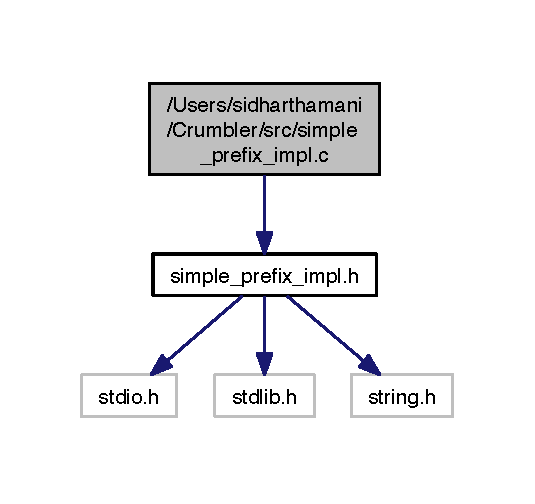
\includegraphics[width=257pt]{simple__prefix__impl_8c__incl}
\end{center}
\end{figure}
\subsection*{Functions}
\begin{DoxyCompactItemize}
\item 
\hyperlink{simple__prefix__impl_8h_structnode}{node} $\ast$ \hyperlink{simple__prefix__impl_8c_ad73cbefe8a90c459159ccc365eb3b33a}{init\-\_\-simple\-\_\-prefix} ()
\begin{DoxyCompactList}\small\item\em allocate memory for a new \hyperlink{structsimple__prefix}{simple\-\_\-prefix} tree \par
 {\bfseries Precondition\-:} The structure should not have already been allocated memory \par
 {\bfseries Postcondition\-:} Memory is allocated and returned to the calling environment \par
 \end{DoxyCompactList}\item 
\hyperlink{simple__prefix__impl_8h_structnode}{node} $\ast$ \hyperlink{simple__prefix__impl_8c_a6657448982edc6daa25abcb440fca1d8}{construct\-\_\-simple\-\_\-prefix\-\_\-tree} (struct \hyperlink{simple__prefix__impl_8h_structnode}{node} $\ast$root, char $\ast$input\-\_\-msgs, int size\-\_\-of\-\_\-input\-\_\-msgs)
\begin{DoxyCompactList}\small\item\em construct a naive \hyperlink{structsimple__prefix}{simple\-\_\-prefix} tree for a set of characters specified by input\-\_\-msgs \par
 {\bfseries  Precondition\-: } Root should have already been initialized \par
 {\bfseries  Postcondition\-: } The Root is initialized to a simple prefix tree for all printable characters \par
 \end{DoxyCompactList}\item 
char $\ast$ \hyperlink{simple__prefix__impl_8c_ab5bd0496da802122958e3af1482d1a6e}{simple\-\_\-prefix\-\_\-encode} (char $\ast$msg, int size\-\_\-of\-\_\-msg)
\begin{DoxyCompactList}\small\item\em encode a string based on the current \hyperlink{structsimple__prefix}{simple\-\_\-prefix} tree, size\-\_\-of\-\_\-msgs(param 2) should be specified in bytes\par
 {\bfseries Precondition \-:} The string into which the returned value should be captured should not have already been allocated. Right now, the function can only encode characters defined in L\-O\-W\-E\-R\-\_\-\-C\-A\-S\-E\-\_\-\-A\-L\-P\-H\-A\-B\-E\-T\-S macro\par
 {\bfseries Postcondition \-:} The message is encoded according to the \hyperlink{structsimple__prefix}{simple\-\_\-prefix} algorithm and returned to the calling environment \end{DoxyCompactList}\item 
char $\ast$ \hyperlink{simple__prefix__impl_8c_a40ee92d324331ee4ca644e67d3697f58}{simple\-\_\-prefix\-\_\-decode} (char $\ast$encoded\-\_\-string, struct \hyperlink{simple__prefix__impl_8h_structnode}{node} $\ast$root, int size\-\_\-of\-\_\-encoded\-\_\-string)
\begin{DoxyCompactList}\small\item\em decode an encoded string by using the prefix tree generated by construct\-\_\-simple\-\_\-prefix(struct node$\ast$, char$\ast$, int) The parameter 2 (struct node$\ast$ root) is a pointer to the generated tree.\par
 {\bfseries Precondition \-:} The tree should have already been generated. The string capturing the return value should not have already been allocated memory\par
 {\bfseries Postcondition \-:} The encoded string is decoded and returned to the calling environment \end{DoxyCompactList}\item 
char $\ast$ \hyperlink{simple__prefix__impl_8c_ac7b35ccc6d71b9a01d2ab3609e20e698}{char2bits} (char $\ast$encoded\-\_\-string, int size\-\_\-of\-\_\-encoded\-\_\-string)
\begin{DoxyCompactList}\small\item\em convert encoded character array into bits for reducing storage space. Use this on an encoded string before persisting this in a file or wherever\par
 {\bfseries Precondition \-:} The string capturing the return value should not have already been allocated memory\par
 {\bfseries Postcondition \-:} The binary representation of the encoded string is returned as an array of bytes(char) \end{DoxyCompactList}\item 
char $\ast$ \hyperlink{simple__prefix__impl_8c_adbcb96421197815cdb34df33d65839c8}{bits2char} (char $\ast$bit\-\_\-stream, int size\-\_\-of\-\_\-bit\-\_\-stream)
\begin{DoxyCompactList}\small\item\em convert encoded bits(as binary data) into a character array for decoding. Use this whenever you read from a persisted source.\-simple\-\_\-prefix\-\_\-decode(char$\ast$, struct node$\ast$, int) undersands encoded strings in char format, not actual binary. Lots of improvement required in this function. Right now, it can only work with the constraint of encoded string length being a multiple of 8.\par
 {\bfseries Precondition \-:} The string capturing the return value should not have already been allocated memory\par
 {\bfseries Postcondition \-:} The character representation of the encoded binary string is returned as an array of bytes(char) \end{DoxyCompactList}\end{DoxyCompactItemize}


\subsection{Detailed Description}
The implementation of \hyperlink{structsimple__prefix}{simple\-\_\-prefix} tree This file contains functions required to support the encoding and de-\/coding functions.\par
 Author \-: Sidhartha Mani\par
 Contact \-: \href{mailto:sidharthamn@gmail.com}{\tt sidharthamn@gmail.\-com} \par
 Last Updated \-: 23 Dec 2012 \par
 

Definition in file \hyperlink{}{simple\-\_\-prefix\-\_\-impl.\-c}.



\subsection{Function Documentation}
\hypertarget{simple__prefix__impl_8c_adbcb96421197815cdb34df33d65839c8}{\index{simple\-\_\-prefix\-\_\-impl.\-c@{simple\-\_\-prefix\-\_\-impl.\-c}!bits2char@{bits2char}}
\index{bits2char@{bits2char}!simple_prefix_impl.c@{simple\-\_\-prefix\-\_\-impl.\-c}}
\subsubsection[{bits2char}]{\setlength{\rightskip}{0pt plus 5cm}char$\ast$ bits2char (
\begin{DoxyParamCaption}
\item[{char $\ast$}]{bit\-\_\-stream, }
\item[{int}]{size\-\_\-of\-\_\-bit\-\_\-stream}
\end{DoxyParamCaption}
)}}\label{simple__prefix__impl_8c_adbcb96421197815cdb34df33d65839c8}


convert encoded bits(as binary data) into a character array for decoding. Use this whenever you read from a persisted source.\-simple\-\_\-prefix\-\_\-decode(char$\ast$, struct node$\ast$, int) undersands encoded strings in char format, not actual binary. Lots of improvement required in this function. Right now, it can only work with the constraint of encoded string length being a multiple of 8.\par
 {\bfseries Precondition \-:} The string capturing the return value should not have already been allocated memory\par
 {\bfseries Postcondition \-:} The character representation of the encoded binary string is returned as an array of bytes(char) 

/fn char$\ast$ \hyperlink{simple__prefix__impl_8c_adbcb96421197815cdb34df33d65839c8}{bits2char(char$\ast$ bit\-\_\-stream, int size\-\_\-of\-\_\-bit\-\_\-stream)} 
\begin{DoxyParams}{Parameters}
{\em bit\-\_\-stream} & bit stream containing the binary encoded information \\
\hline
{\em size\-\_\-of\-\_\-bit\-\_\-stream} & size of the bit\-\_\-stream \\
\hline
\end{DoxyParams}
\begin{DoxyReturn}{Returns}
an array of bytes(char) containing each bit of param 1(bit\-\_\-stream) as a character, as required by \hyperlink{simple__prefix__impl_8c_a40ee92d324331ee4ca644e67d3697f58}{simple\-\_\-prefix\-\_\-decode(char$\ast$, struct node$\ast$, int)}
\end{DoxyReturn}

\begin{DoxyParams}{Parameters}
{\em bit\-\_\-stream} & bit stream containing the binary encoded information \\
\hline
{\em size\-\_\-of\-\_\-bit\-\_\-stream} & size of the bit\-\_\-stream \\
\hline
\end{DoxyParams}
\begin{DoxyReturn}{Returns}
an array of bytes(char) containing each bit of param 1(bit\-\_\-stream) as a character, as required by \hyperlink{simple__prefix__impl_8c_a40ee92d324331ee4ca644e67d3697f58}{simple\-\_\-prefix\-\_\-decode(char$\ast$, struct node$\ast$, int)} 
\end{DoxyReturn}


Definition at line 240 of file simple\-\_\-prefix\-\_\-impl.\-c.


\begin{DoxyCode}
\{
    \textcolor{keywordtype}{char} *encoded\_string = (\textcolor{keywordtype}{char} *)malloc(strlen(bit\_stream)*8 + 1);
    \textcolor{keywordtype}{int} i = 0;
    \textcolor{keywordtype}{int} j = 0;
    \textcolor{keywordtype}{int} k = size\_of\_bit\_stream*8 - 1;
    encoded\_string[k+1] = \textcolor{charliteral}{'\(\backslash\)0'};
    \textcolor{keywordtype}{char} bit;
    \textcolor{keywordflow}{for}(i = 0;i<size\_of\_bit\_stream;i++)
    \{
        bit = bit\_stream[i];
        \textcolor{keywordflow}{for} (j=0; j<8; j++) 
        \{
            \textcolor{keywordflow}{if} (bit & 1) 
            \{
                encoded\_string[k--] = \textcolor{charliteral}{'1'};
            \}
            \textcolor{keywordflow}{else} 
            \{
                encoded\_string[k--] = \textcolor{charliteral}{'0'};
            \}
            bit >>= 1;
        \}
    \}
    \textcolor{keywordflow}{return} encoded\_string;
\}
\end{DoxyCode}
\hypertarget{simple__prefix__impl_8c_ac7b35ccc6d71b9a01d2ab3609e20e698}{\index{simple\-\_\-prefix\-\_\-impl.\-c@{simple\-\_\-prefix\-\_\-impl.\-c}!char2bits@{char2bits}}
\index{char2bits@{char2bits}!simple_prefix_impl.c@{simple\-\_\-prefix\-\_\-impl.\-c}}
\subsubsection[{char2bits}]{\setlength{\rightskip}{0pt plus 5cm}char$\ast$ char2bits (
\begin{DoxyParamCaption}
\item[{char $\ast$}]{encoded\-\_\-string, }
\item[{int}]{size\-\_\-of\-\_\-encoded\-\_\-string}
\end{DoxyParamCaption}
)}}\label{simple__prefix__impl_8c_ac7b35ccc6d71b9a01d2ab3609e20e698}


convert encoded character array into bits for reducing storage space. Use this on an encoded string before persisting this in a file or wherever\par
 {\bfseries Precondition \-:} The string capturing the return value should not have already been allocated memory\par
 {\bfseries Postcondition \-:} The binary representation of the encoded string is returned as an array of bytes(char) 

/fn char$\ast$ \hyperlink{simple__prefix__impl_8c_ac7b35ccc6d71b9a01d2ab3609e20e698}{char2bits(char$\ast$ encoded\-\_\-string, int size\-\_\-of\-\_\-encoded\-\_\-string)} 
\begin{DoxyParams}{Parameters}
{\em encoded\-\_\-string} & The string to be converted into binary \\
\hline
{\em size\-\_\-of\-\_\-encoded\-\_\-string} & the size of the string in param 1 \\
\hline
\end{DoxyParams}
\begin{DoxyReturn}{Returns}
a bit stream containing the binary information encoded in param 1(encoded\-\_\-string)
\end{DoxyReturn}

\begin{DoxyParams}{Parameters}
{\em encoded\-\_\-string} & The string to be converted into binary \\
\hline
{\em size\-\_\-of\-\_\-encoded\-\_\-string} & the size of the string in param 1 \\
\hline
\end{DoxyParams}
\begin{DoxyReturn}{Returns}
a bit stream containing the binary information encoded in param 1(encoded\-\_\-string) 
\end{DoxyReturn}


Definition at line 209 of file simple\-\_\-prefix\-\_\-impl.\-c.


\begin{DoxyCode}
\{
    \textcolor{keywordtype}{char} *bit\_stream = (\textcolor{keywordtype}{char} *)malloc(size\_of\_encoded\_string/8 + 2);
    \textcolor{keywordtype}{char} bit = 0;
    \textcolor{keywordtype}{int} i = 0;
    \textcolor{keywordtype}{int} j = 0;
    \textcolor{keywordflow}{for} (i=0; i<size\_of\_encoded\_string; i++) 
    \{
        bit |= (int)((\textcolor{keywordtype}{int})encoded\_string[i] - (int)\textcolor{charliteral}{'0'});
        \textcolor{keywordflow}{if} ((i+1)%8 == 0) 
        \{
            bit\_stream[j++] = bit;
            bit = 0;
        \}
        bit <<= 1;
    \}
    \textcolor{keywordflow}{return} bit\_stream;
\}
\end{DoxyCode}
\hypertarget{simple__prefix__impl_8c_a6657448982edc6daa25abcb440fca1d8}{\index{simple\-\_\-prefix\-\_\-impl.\-c@{simple\-\_\-prefix\-\_\-impl.\-c}!construct\-\_\-simple\-\_\-prefix\-\_\-tree@{construct\-\_\-simple\-\_\-prefix\-\_\-tree}}
\index{construct\-\_\-simple\-\_\-prefix\-\_\-tree@{construct\-\_\-simple\-\_\-prefix\-\_\-tree}!simple_prefix_impl.c@{simple\-\_\-prefix\-\_\-impl.\-c}}
\subsubsection[{construct\-\_\-simple\-\_\-prefix\-\_\-tree}]{\setlength{\rightskip}{0pt plus 5cm}{\bf node}$\ast$ construct\-\_\-simple\-\_\-prefix\-\_\-tree (
\begin{DoxyParamCaption}
\item[{struct {\bf node} $\ast$}]{root, }
\item[{char $\ast$}]{input\-\_\-msgs, }
\item[{int}]{size\-\_\-of\-\_\-input\-\_\-msgs}
\end{DoxyParamCaption}
)}}\label{simple__prefix__impl_8c_a6657448982edc6daa25abcb440fca1d8}


construct a naive \hyperlink{structsimple__prefix}{simple\-\_\-prefix} tree for a set of characters specified by input\-\_\-msgs \par
 {\bfseries  Precondition\-: } Root should have already been initialized \par
 {\bfseries  Postcondition\-: } The Root is initialized to a simple prefix tree for all printable characters \par
 


\begin{DoxyParams}{Parameters}
{\em root} & A pointer to the root of the tree. It is essentially a pointer to the entire tree. \\
\hline
{\em input\-\_\-msgs} & An array of characters for which the tree is being built. \par
 {\bfseries Note \-:} The letters that occur earlier in the input\-\_\-msgs array will have a lower encoded length than the letters that occur later in the input\-\_\-msgs array. \\
\hline
{\em size\-\_\-of\-\_\-input\-\_\-msgs} & The length of the input\-\_\-msgs array \\
\hline
\end{DoxyParams}
\begin{DoxyReturn}{Returns}
it returns the root of the constructed prefix tree 
\end{DoxyReturn}


Definition at line 47 of file simple\-\_\-prefix\-\_\-impl.\-c.


\begin{DoxyCode}
\{
    \textcolor{comment}{//definition : Naive simple\_prefix tree  -  a simple\_prefix tree that is
       constructed without considering}
    \textcolor{comment}{//the probabilites of messages. A lower length prefix code is given to a
       message }
    \textcolor{comment}{//if it occurs before another message while processing. That is, a msg
       whose index is lower}
    \textcolor{comment}{//in the input\_msgs array will have a shorter prefix code than a msg that
       has a higher array }
    \textcolor{comment}{//index}
    \textcolor{keywordtype}{int} i = 0;
    \textcolor{keyword}{struct }\hyperlink{simple__prefix__impl_8h_structnode}{node} *temp =  root;
    \textcolor{keywordflow}{for} (i = 0; i<size\_of\_input\_msgs; i++) 
    \{
        \textcolor{keywordflow}{while} (temp->\hyperlink{simple__prefix__impl_8h_a43dd3cf499d5b2270fcfbb29eb0a0d66}{left\_node} != NULL) 
        \{
            temp = temp->\hyperlink{simple__prefix__impl_8h_a43dd3cf499d5b2270fcfbb29eb0a0d66}{left\_node};
        \}
        \textcolor{keywordflow}{if} (temp->\hyperlink{simple__prefix__impl_8h_af729d9e66cefdd8c0a114cb0da5f7b7c}{right\_node} == NULL && temp == root) 
        \{
            \textcolor{keyword}{struct }\hyperlink{simple__prefix__impl_8h_structnode}{node} *new\_node = (\textcolor{keyword}{struct }\hyperlink{simple__prefix__impl_8h_structnode}{node} *)malloc(\textcolor{keyword}{sizeof}(\textcolor{keyword}{struct}
       \hyperlink{simple__prefix__impl_8h_structnode}{node}));
            new\_node->\hyperlink{simple__prefix__impl_8h_ad80e777cd260fdd5ca6ad3f25b5e76de}{msg} = input\_msgs[i];
            temp->\hyperlink{simple__prefix__impl_8h_af729d9e66cefdd8c0a114cb0da5f7b7c}{right\_node} = new\_node;
            new\_node->\hyperlink{simple__prefix__impl_8h_a43dd3cf499d5b2270fcfbb29eb0a0d66}{left\_node} = NULL;
            new\_node->\hyperlink{simple__prefix__impl_8h_af729d9e66cefdd8c0a114cb0da5f7b7c}{right\_node} = NULL;
            new\_node->\hyperlink{simple__prefix__impl_8h_ad066657fe1374fb9852c285175a3774f}{is\_leaf} = 1;
        \}
        \textcolor{keywordflow}{else} \textcolor{keywordflow}{if} (temp->\hyperlink{simple__prefix__impl_8h_a43dd3cf499d5b2270fcfbb29eb0a0d66}{left\_node} == NULL && temp == root) 
        \{
            \textcolor{keyword}{struct }\hyperlink{simple__prefix__impl_8h_structnode}{node} *new\_node = (\textcolor{keyword}{struct }\hyperlink{simple__prefix__impl_8h_structnode}{node} *)malloc(\textcolor{keyword}{sizeof}(\textcolor{keyword}{struct}
       \hyperlink{simple__prefix__impl_8h_structnode}{node}));
            new\_node->\hyperlink{simple__prefix__impl_8h_ad80e777cd260fdd5ca6ad3f25b5e76de}{msg} = input\_msgs[i];
            temp->\hyperlink{simple__prefix__impl_8h_a43dd3cf499d5b2270fcfbb29eb0a0d66}{left\_node} = new\_node;
            new\_node->\hyperlink{simple__prefix__impl_8h_a43dd3cf499d5b2270fcfbb29eb0a0d66}{left\_node} = NULL;
            new\_node->\hyperlink{simple__prefix__impl_8h_af729d9e66cefdd8c0a114cb0da5f7b7c}{right\_node} = NULL;
            new\_node->\hyperlink{simple__prefix__impl_8h_ad066657fe1374fb9852c285175a3774f}{is\_leaf} = 1;
        \}
        \textcolor{keywordflow}{else} \textcolor{keywordflow}{if} (temp->\hyperlink{simple__prefix__impl_8h_af729d9e66cefdd8c0a114cb0da5f7b7c}{right\_node} == NULL)
        \{
            \textcolor{keyword}{struct }\hyperlink{simple__prefix__impl_8h_structnode}{node} *new\_node = (\textcolor{keyword}{struct }\hyperlink{simple__prefix__impl_8h_structnode}{node} *)malloc(\textcolor{keyword}{sizeof}(\textcolor{keyword}{struct}
       \hyperlink{simple__prefix__impl_8h_structnode}{node}));
            new\_node->\hyperlink{simple__prefix__impl_8h_ad80e777cd260fdd5ca6ad3f25b5e76de}{msg} = temp->\hyperlink{simple__prefix__impl_8h_ad80e777cd260fdd5ca6ad3f25b5e76de}{msg};
            temp->\hyperlink{simple__prefix__impl_8h_ad066657fe1374fb9852c285175a3774f}{is\_leaf} = 0;
            temp->\hyperlink{simple__prefix__impl_8h_af729d9e66cefdd8c0a114cb0da5f7b7c}{right\_node} = new\_node;
            new\_node->\hyperlink{simple__prefix__impl_8h_a43dd3cf499d5b2270fcfbb29eb0a0d66}{left\_node} = NULL;
            new\_node->\hyperlink{simple__prefix__impl_8h_af729d9e66cefdd8c0a114cb0da5f7b7c}{right\_node} = NULL;
            new\_node->\hyperlink{simple__prefix__impl_8h_ad066657fe1374fb9852c285175a3774f}{is\_leaf} = 1;
            \textcolor{keyword}{struct }\hyperlink{simple__prefix__impl_8h_structnode}{node} *new\_node\_2 = (\textcolor{keyword}{struct }\hyperlink{simple__prefix__impl_8h_structnode}{node} *)malloc(\textcolor{keyword}{sizeof}(\textcolor{keyword}{
      struct} \hyperlink{simple__prefix__impl_8h_structnode}{node}));
            temp->\hyperlink{simple__prefix__impl_8h_a43dd3cf499d5b2270fcfbb29eb0a0d66}{left\_node} = new\_node\_2;
            new\_node\_2->\hyperlink{simple__prefix__impl_8h_ad80e777cd260fdd5ca6ad3f25b5e76de}{msg} = input\_msgs[i];
            new\_node\_2->\hyperlink{simple__prefix__impl_8h_ad066657fe1374fb9852c285175a3774f}{is\_leaf} = 1;
            new\_node\_2->\hyperlink{simple__prefix__impl_8h_a43dd3cf499d5b2270fcfbb29eb0a0d66}{left\_node} = NULL;
            new\_node\_2->\hyperlink{simple__prefix__impl_8h_af729d9e66cefdd8c0a114cb0da5f7b7c}{right\_node} = NULL;
        \}
    \}
    \textcolor{keywordflow}{return} root;
\}
\end{DoxyCode}
\hypertarget{simple__prefix__impl_8c_ad73cbefe8a90c459159ccc365eb3b33a}{\index{simple\-\_\-prefix\-\_\-impl.\-c@{simple\-\_\-prefix\-\_\-impl.\-c}!init\-\_\-simple\-\_\-prefix@{init\-\_\-simple\-\_\-prefix}}
\index{init\-\_\-simple\-\_\-prefix@{init\-\_\-simple\-\_\-prefix}!simple_prefix_impl.c@{simple\-\_\-prefix\-\_\-impl.\-c}}
\subsubsection[{init\-\_\-simple\-\_\-prefix}]{\setlength{\rightskip}{0pt plus 5cm}{\bf node}$\ast$ init\-\_\-simple\-\_\-prefix (
\begin{DoxyParamCaption}
{}
\end{DoxyParamCaption}
)}}\label{simple__prefix__impl_8c_ad73cbefe8a90c459159ccc365eb3b33a}


allocate memory for a new \hyperlink{structsimple__prefix}{simple\-\_\-prefix} tree \par
 {\bfseries Precondition\-:} The structure should not have already been allocated memory \par
 {\bfseries Postcondition\-:} Memory is allocated and returned to the calling environment \par
 

\begin{DoxyReturn}{Returns}
A pointer to the allocated memory 
\end{DoxyReturn}


Definition at line 26 of file simple\-\_\-prefix\-\_\-impl.\-c.


\begin{DoxyCode}
\{
    \textcolor{keyword}{struct }\hyperlink{simple__prefix__impl_8h_structnode}{node} *root = (\textcolor{keyword}{struct }\hyperlink{simple__prefix__impl_8h_structnode}{node} *)malloc(\textcolor{keyword}{sizeof}(\textcolor{keyword}{struct} \hyperlink{simple__prefix__impl_8h_structnode}{node}));
    root->\hyperlink{simple__prefix__impl_8h_ad066657fe1374fb9852c285175a3774f}{is\_leaf} = 0;
    root->\hyperlink{simple__prefix__impl_8h_a43dd3cf499d5b2270fcfbb29eb0a0d66}{left\_node} = NULL;
    root->\hyperlink{simple__prefix__impl_8h_af729d9e66cefdd8c0a114cb0da5f7b7c}{right\_node} = NULL;
    \textcolor{keywordflow}{return} root;
\}
\end{DoxyCode}
\hypertarget{simple__prefix__impl_8c_a40ee92d324331ee4ca644e67d3697f58}{\index{simple\-\_\-prefix\-\_\-impl.\-c@{simple\-\_\-prefix\-\_\-impl.\-c}!simple\-\_\-prefix\-\_\-decode@{simple\-\_\-prefix\-\_\-decode}}
\index{simple\-\_\-prefix\-\_\-decode@{simple\-\_\-prefix\-\_\-decode}!simple_prefix_impl.c@{simple\-\_\-prefix\-\_\-impl.\-c}}
\subsubsection[{simple\-\_\-prefix\-\_\-decode}]{\setlength{\rightskip}{0pt plus 5cm}char$\ast$ simple\-\_\-prefix\-\_\-decode (
\begin{DoxyParamCaption}
\item[{char $\ast$}]{encoded\-\_\-string, }
\item[{struct {\bf node} $\ast$}]{root, }
\item[{int}]{size\-\_\-of\-\_\-encoded\-\_\-string}
\end{DoxyParamCaption}
)}}\label{simple__prefix__impl_8c_a40ee92d324331ee4ca644e67d3697f58}


decode an encoded string by using the prefix tree generated by construct\-\_\-simple\-\_\-prefix(struct node$\ast$, char$\ast$, int) The parameter 2 (struct node$\ast$ root) is a pointer to the generated tree.\par
 {\bfseries Precondition \-:} The tree should have already been generated. The string capturing the return value should not have already been allocated memory\par
 {\bfseries Postcondition \-:} The encoded string is decoded and returned to the calling environment 


\begin{DoxyParams}{Parameters}
{\em encoded\-\_\-string} & the encoded string as an array of characters, not as binary data \\
\hline
{\em root} & the \hyperlink{structsimple__prefix}{simple\-\_\-prefix} tree needed by the decoding algorithm \\
\hline
{\em size\-\_\-of\-\_\-encoded\-\_\-string} & the size of the encoded string \\
\hline
\end{DoxyParams}
\begin{DoxyReturn}{Returns}
the decoded string 
\end{DoxyReturn}


Definition at line 170 of file simple\-\_\-prefix\-\_\-impl.\-c.


\begin{DoxyCode}
\{
    \textcolor{keywordtype}{char} *decoded\_string = (\textcolor{keywordtype}{char} *)malloc(size\_of\_encoded\_string);
    \textcolor{keywordtype}{int} i = 0;
    \textcolor{keywordtype}{int} j = 0;
    \textcolor{keyword}{struct }\hyperlink{simple__prefix__impl_8h_structnode}{node} *temp;
    \textcolor{keywordflow}{while}(i < size\_of\_encoded\_string)
    \{
        \textcolor{comment}{//iterate through each node until you reach the encoded character}
        temp = root;
        \textcolor{keywordflow}{while}(temp->\hyperlink{simple__prefix__impl_8h_ad066657fe1374fb9852c285175a3774f}{is\_leaf} != 1 && i < size\_of\_encoded\_string)
        \{
            \textcolor{keywordflow}{if}(encoded\_string[i] == \textcolor{charliteral}{'0'})
            \{
                temp = temp->\hyperlink{simple__prefix__impl_8h_a43dd3cf499d5b2270fcfbb29eb0a0d66}{left\_node};
            \}
            \textcolor{keywordflow}{else}
            \{
                temp = temp->\hyperlink{simple__prefix__impl_8h_af729d9e66cefdd8c0a114cb0da5f7b7c}{right\_node};
            \}
            i++;
        \}
        decoded\_string[j++] = temp->\hyperlink{simple__prefix__impl_8h_ad80e777cd260fdd5ca6ad3f25b5e76de}{msg};
    \}
    \textcolor{comment}{//finish the string}
    decoded\_string[j] = \textcolor{charliteral}{'\(\backslash\)0'};
    \textcolor{keywordflow}{return} decoded\_string;
\}
\end{DoxyCode}
\hypertarget{simple__prefix__impl_8c_ab5bd0496da802122958e3af1482d1a6e}{\index{simple\-\_\-prefix\-\_\-impl.\-c@{simple\-\_\-prefix\-\_\-impl.\-c}!simple\-\_\-prefix\-\_\-encode@{simple\-\_\-prefix\-\_\-encode}}
\index{simple\-\_\-prefix\-\_\-encode@{simple\-\_\-prefix\-\_\-encode}!simple_prefix_impl.c@{simple\-\_\-prefix\-\_\-impl.\-c}}
\subsubsection[{simple\-\_\-prefix\-\_\-encode}]{\setlength{\rightskip}{0pt plus 5cm}char$\ast$ simple\-\_\-prefix\-\_\-encode (
\begin{DoxyParamCaption}
\item[{char $\ast$}]{msg, }
\item[{int}]{size\-\_\-of\-\_\-msg}
\end{DoxyParamCaption}
)}}\label{simple__prefix__impl_8c_ab5bd0496da802122958e3af1482d1a6e}


encode a string based on the current \hyperlink{structsimple__prefix}{simple\-\_\-prefix} tree, size\-\_\-of\-\_\-msgs(param 2) should be specified in bytes\par
 {\bfseries Precondition \-:} The string into which the returned value should be captured should not have already been allocated. Right now, the function can only encode characters defined in L\-O\-W\-E\-R\-\_\-\-C\-A\-S\-E\-\_\-\-A\-L\-P\-H\-A\-B\-E\-T\-S macro\par
 {\bfseries Postcondition \-:} The message is encoded according to the \hyperlink{structsimple__prefix}{simple\-\_\-prefix} algorithm and returned to the calling environment 


\begin{DoxyParams}{Parameters}
{\em msg} & the string that needs to be encoded \\
\hline
{\em size\-\_\-of\-\_\-msg} & the length of the message \\
\hline
\end{DoxyParams}
\begin{DoxyReturn}{Returns}
a pointer to the encoded message. \par
 The returned encoded message is not in binary, it is still a character array. It can be converted into binary using \hyperlink{simple__prefix__impl_8c_ac7b35ccc6d71b9a01d2ab3609e20e698}{char2bits(char $\ast$, int)} function 
\end{DoxyReturn}


Definition at line 112 of file simple\-\_\-prefix\-\_\-impl.\-c.


\begin{DoxyCode}
\{
    \textcolor{keywordtype}{char} conversion\_tree[][27] = \{
        \textcolor{stringliteral}{"1"}, \textcolor{comment}{//e}
        \textcolor{stringliteral}{"01"}, \textcolor{comment}{//a}
        \textcolor{stringliteral}{"001"}, \textcolor{comment}{//r}
        \textcolor{stringliteral}{"0001"}, \textcolor{comment}{//i}
        \textcolor{stringliteral}{"00001"}, \textcolor{comment}{//o}
        \textcolor{stringliteral}{"000001"}, \textcolor{comment}{//t}
        \textcolor{stringliteral}{"0000001"}, \textcolor{comment}{//n}
        \textcolor{stringliteral}{"00000001"}, \textcolor{comment}{//s}
        \textcolor{stringliteral}{"000000001"}, \textcolor{comment}{//l}
        \textcolor{stringliteral}{"0000000001"}, \textcolor{comment}{//c}
        \textcolor{stringliteral}{"00000000001"}, \textcolor{comment}{//u}
        \textcolor{stringliteral}{"000000000001"}, \textcolor{comment}{//d}
        \textcolor{stringliteral}{"0000000000001"}, \textcolor{comment}{//p}
        \textcolor{stringliteral}{"00000000000001"}, \textcolor{comment}{//m}
        \textcolor{stringliteral}{"000000000000001"}, \textcolor{comment}{//h}
        \textcolor{stringliteral}{"0000000000000001"}, \textcolor{comment}{//g}
        \textcolor{stringliteral}{"00000000000000001"}, \textcolor{comment}{//b}
        \textcolor{stringliteral}{"000000000000000001"}, \textcolor{comment}{//f}
        \textcolor{stringliteral}{"0000000000000000001"}, \textcolor{comment}{//y}
        \textcolor{stringliteral}{"00000000000000000001"}, \textcolor{comment}{//w}
        \textcolor{stringliteral}{"000000000000000000001"}, \textcolor{comment}{//k}
        \textcolor{stringliteral}{"0000000000000000000001"}, \textcolor{comment}{//v}
        \textcolor{stringliteral}{"00000000000000000000001"}, \textcolor{comment}{//x}
        \textcolor{stringliteral}{"000000000000000000000001"}, \textcolor{comment}{//z}
        \textcolor{stringliteral}{"0000000000000000000000001"}, \textcolor{comment}{//j}
        \textcolor{stringliteral}{"00000000000000000000000001"}, \textcolor{comment}{//q}
        \textcolor{stringliteral}{"00000000000000000000000000"} \textcolor{comment}{//WHITE SPACE}
    \};
    \textcolor{keywordtype}{char} *encoded\_string = (\textcolor{keywordtype}{char} *)malloc(27*size\_of\_msg);
    \textcolor{keywordtype}{int} i = 0;
    \textcolor{keywordtype}{char} reference\_string[] = \hyperlink{simple__prefix__impl_8h_a94747a3d988297667d1f086be19a7f3d}{LOWER\_CASE\_ALPHABETS};
    \textcolor{keywordflow}{while} (i < size\_of\_msg) 
    \{
    \textcolor{comment}{//ignore un-recognized characters}
    \textcolor{keywordflow}{if} ((\textcolor{keywordtype}{int})((strchr(reference\_string,\hyperlink{simple__prefix__impl_8h_ad80e777cd260fdd5ca6ad3f25b5e76de}{msg}[i])) - reference\_string) < 0 || (
      int)((strchr(reference\_string,\hyperlink{simple__prefix__impl_8h_ad80e777cd260fdd5ca6ad3f25b5e76de}{msg}[i])) - reference\_string) > 26) \{
        i++;
        \textcolor{keywordflow}{continue};
    \}
    encoded\_string = strcat(encoded\_string,conversion\_tree[(\textcolor{keywordtype}{int})((strchr(
      reference\_string,\hyperlink{simple__prefix__impl_8h_ad80e777cd260fdd5ca6ad3f25b5e76de}{msg}[i])) - reference\_string)]);
    i++;
    \}
    \textcolor{keywordflow}{return} encoded\_string;
\}
\end{DoxyCode}

\addcontentsline{toc}{part}{Index}
\printindex
\end{document}
